\chapter{Swarm type identification}\label{chapter:SwarmType}
%%\section{Metric application - swarm type identification\label{methods:SwarmTypesStability1}}
This chapter applies the metrics defined in chapter~\ref{chapter:metric} to identify how the cohesion and repulsion field effects of the \textit{interaction vector} affect the internal movement and the vector magnitudes between agents in a swarm. 

There are two distinct inter-agent structures that can emerge in a boid-based swarm, \textit{hexagonally-connected} or \textit{hyper-connected}. These two swarm types are the result of the cohesion field effect detecting immediate neighbours only and when the neighbour field effect range extends beyond immediate neighbours to include additional agents. 

If the goal is to maximise the coverage of an area by a swarm's agents then a hexagonal lattice is the most appropriate structure. In a \textit{hexagonally-connected} swarm agents have visibility only of their immediate neighbours and are unaffected by agents beyond those neighbours. This effect can be implemented by ignoring agents beyond the initial neighbours detected or confining the field effects such that the connections do not occur. If the field effects extend beyond the immediate neighbours such that further agents are detected then there will be additional vectors affecting the calculations of an agent's \textit{interaction vectors}. These additional vectors cause the structure to change logically from a lattice to a mesh. A mesh structure is a \textit{hyper-connected} swarm.

\section{Internal movement testing (static swarms)}\label{Section:StabilityTesting}
To evaluate the metrics simulation parameters (field effects) need to be created such that they generate the two swarm types~(\autoref{tab:Physics2}).

Table~\ref{tab:Physics2} shows the parameter requirements for two swarm types. The parameters in the \textit{Hexagonal} column generate a swarm structure where an agent can only detect immediate neighbours. The parameters in the \textit{Hyper} column allow agents to detect agents beyond their immediate neighbours and therefore create additional neighbour connections which results in a hyper-connected swarm.

\begin{table}[H]
\begin{center}
\begin{tabular}{| p{2.5cm} | K{2.5cm} | K{2.5cm} | p{4.5cm} |}
\hline
\bf Weight \bf component & \bf Hexagonal \bf Swarm & \bf Hyper \bf connected & \bf Description \\ \hline
Sample Rate & 100 & 100 & ms - Unit sampling interval\\  \hline
$k_c$ & 5 & 5 & weight adjuster for cohesion bias\\  \hline
$k_r$ & 15 & 15 & weight adjuster for repulsion  bias\\  \hline
$k_d$ & 0 & 0 & weight adjuster for directional bias\\  \hline
Cohesion field & 50 & 60 &  units\\  \hline
Repulsion field & 40 & 40 & units\\  \hline
Speed & 20 & 20 & units/s\\  \hline
\end{tabular}\caption{Swarm Weighted Model} \label{tab:Physics2}
\end{center}
\end{table}

The two sets of parameters are simulated using a swarm of 200 agents randomly distributed in an environment. The simulation generates data as described in chapter~\ref{chapter:simulator}. The data extracts contain the distances and inter-agent magnitudes (\textit{interaction vectors}) produced by the parameters.

\section{Hexagonal swarm analysis}\label{section:AnalysisA}
In a hexagonal swarm the field effects cause the agents to form a regular lattice. All the agents tend towards an even distributed with similar distances between each agent and its neighbours. In a well structured deployment, the agents in the swarm will show limited variation in the inter-agent distances and the \textit{interaction vectors}. A perfect distribution is very unlikely in a swarm of agents due to the constant movement of the agents adjusting their positions to obtain an optimum position and the agents moving at a constant speed.

\subsection{Distance based metric}
The distance analysis graph~(\autoref{methods:StabilityDistanceSwarm40-50}) for the hexagonal swarm (using the parameters in Table~\ref{tab:Physics2}, repulsion field 40 units, cohesion field 60 units) shows the distance metric being applied to the swarm over a period of 200 cycles. The graph shows a trace of the distance with the standard deviation displayed as error bars above and below the mean.

The swarm is initially (0-20 cycles) in a state of disorganisation, where the agent distribution is varied. The swarm then enters a phase where the hexagons are forming and the swarm starts to stablise (20-50 cycles). After about 50 cycles the field effects have stabilised the swarm structure and the swarm settles to a more stable state for the given set of parameters. The swarm then fluctuates as the residual internal movement maintains the swarm's structure. At this point the internal movement (jitter) is the `background noise' generated by the field effects to maintain the swarm's structure.

%HEX-DIST.py
\begin{figure}[H]
\begin{center}
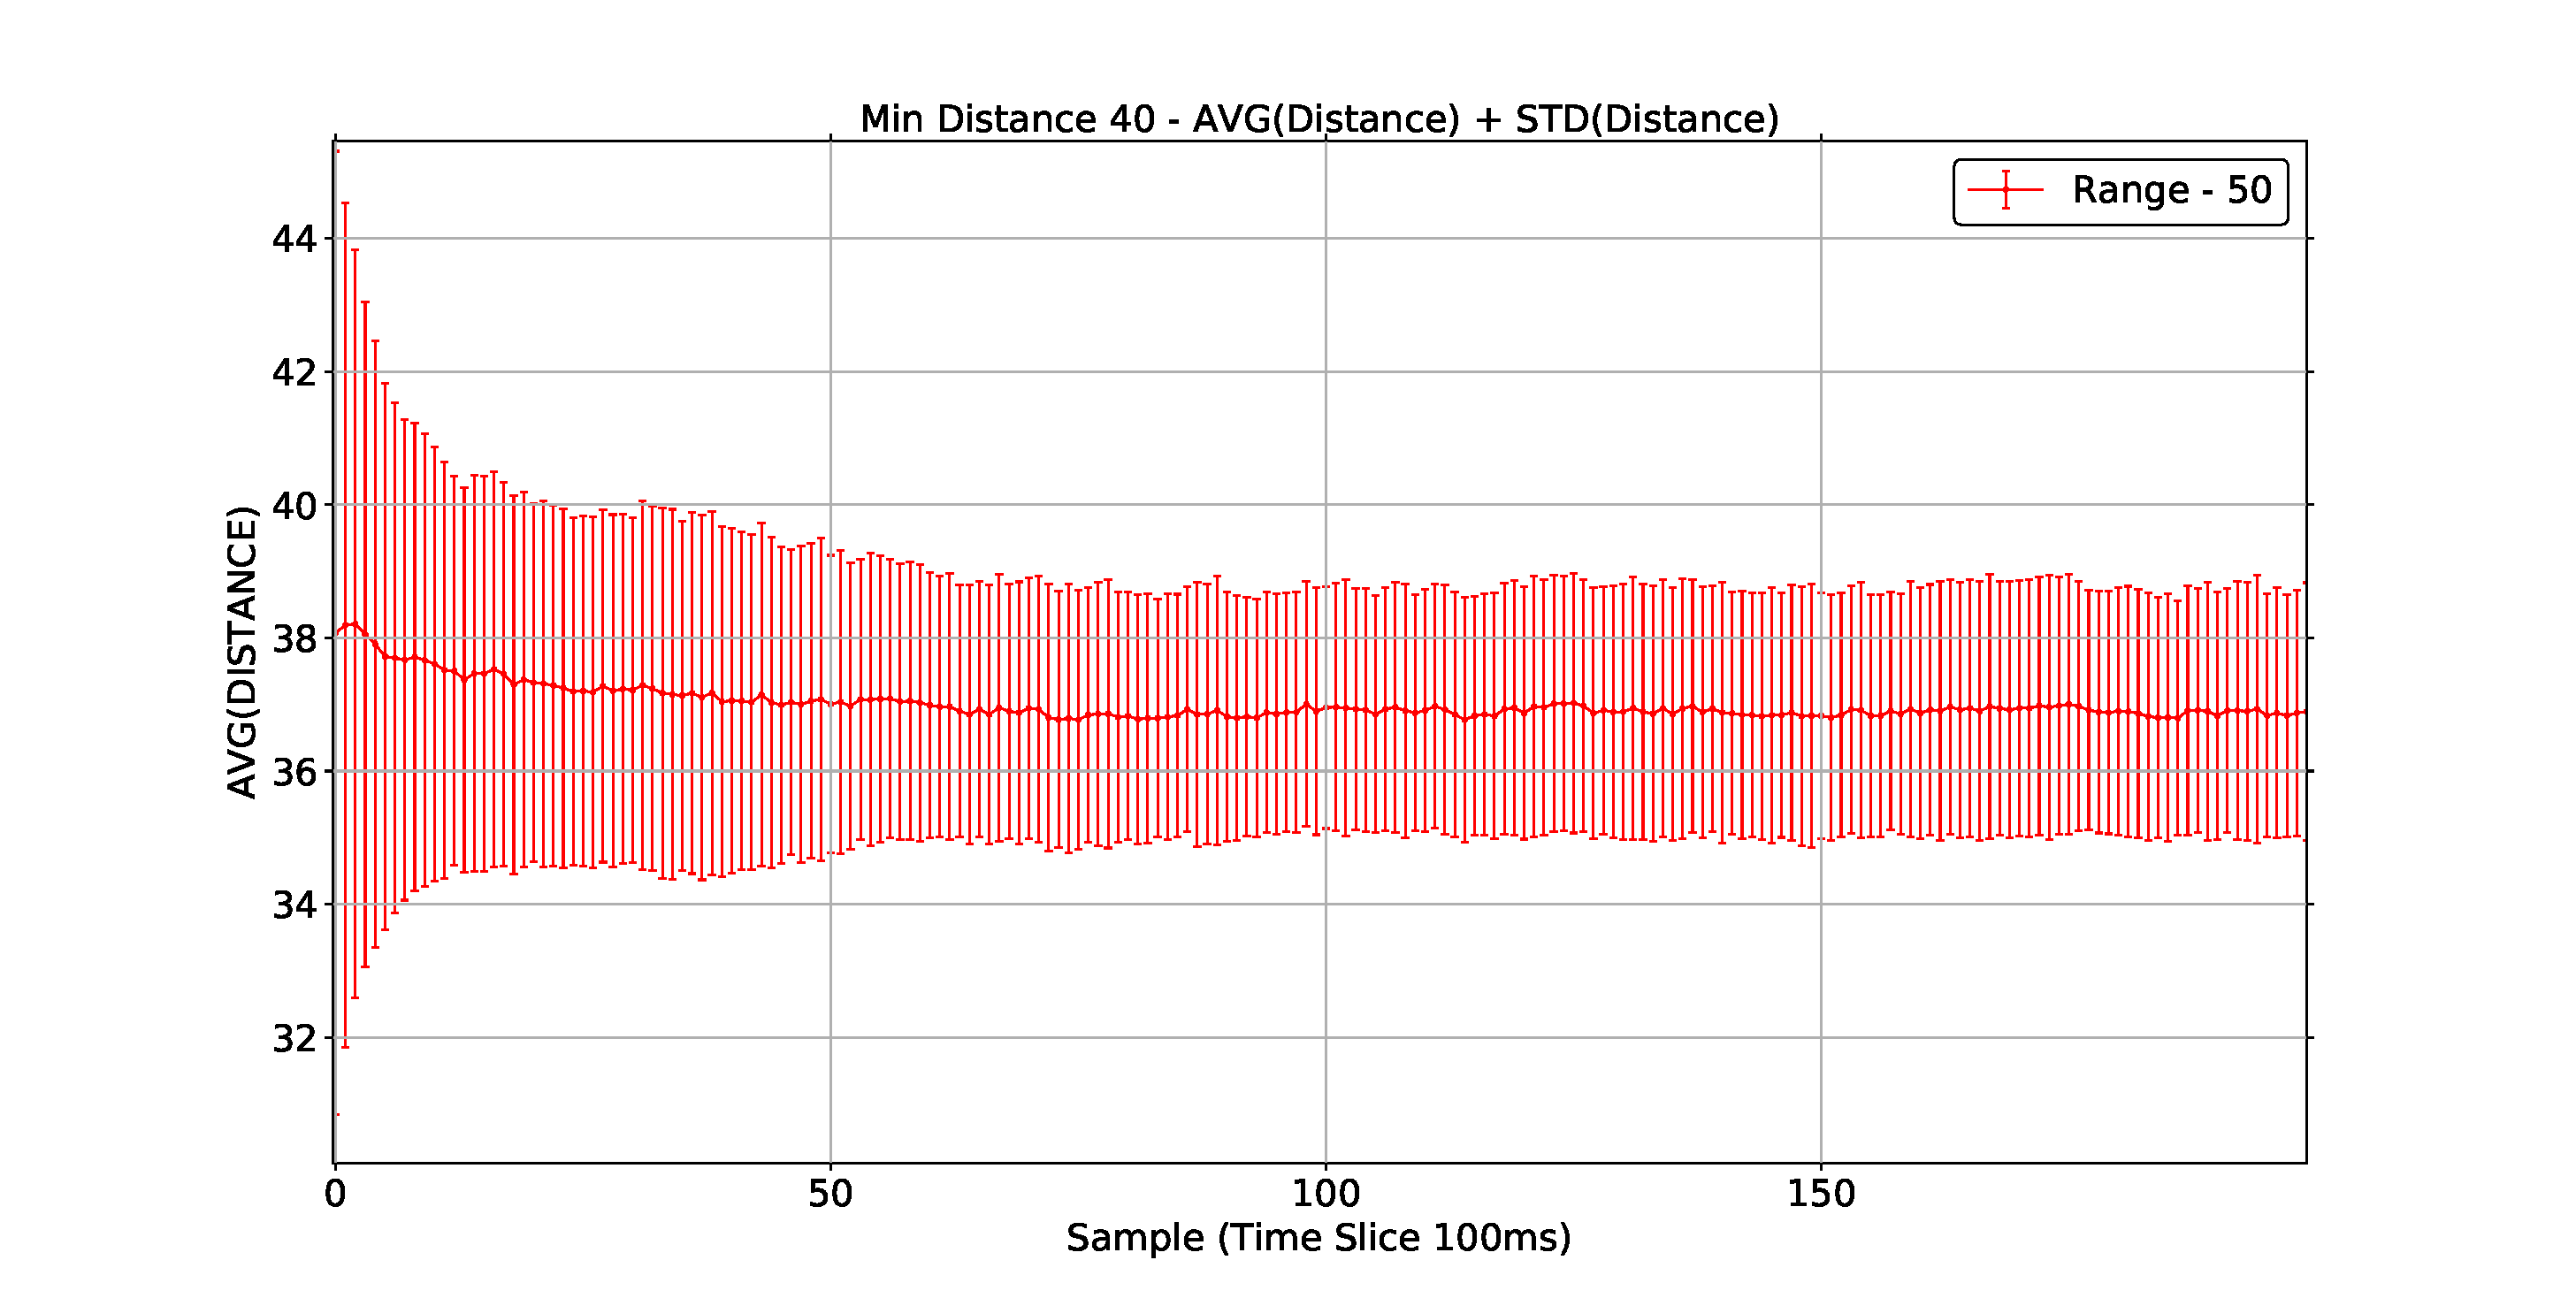
\includegraphics[width=13cm]{CHAPTER-5/figures/StabilityDistanceSwarm40-50}
\end{center}
\caption{Hexagonal swarm - distance metric\label{methods:StabilityDistanceSwarm40-50}}
\end{figure}

\autoref{methods:StabilityDistributionHexagonal}~shows the distribution of the inter-agent distances for the duration of the simulation. The data forms a bell shaped distribution with a mean distance of approximately 37 units, the mean distance is the average of all the inter agent distances as shown in \autoref{methods:StabilityDistanceSwarm40-50}. The graph shows the changes in the distribution of distances based on the aggregation of the whole simulation. 
%HEX-DIST-BAR.py
\begin{figure}[H]
\begin{center}
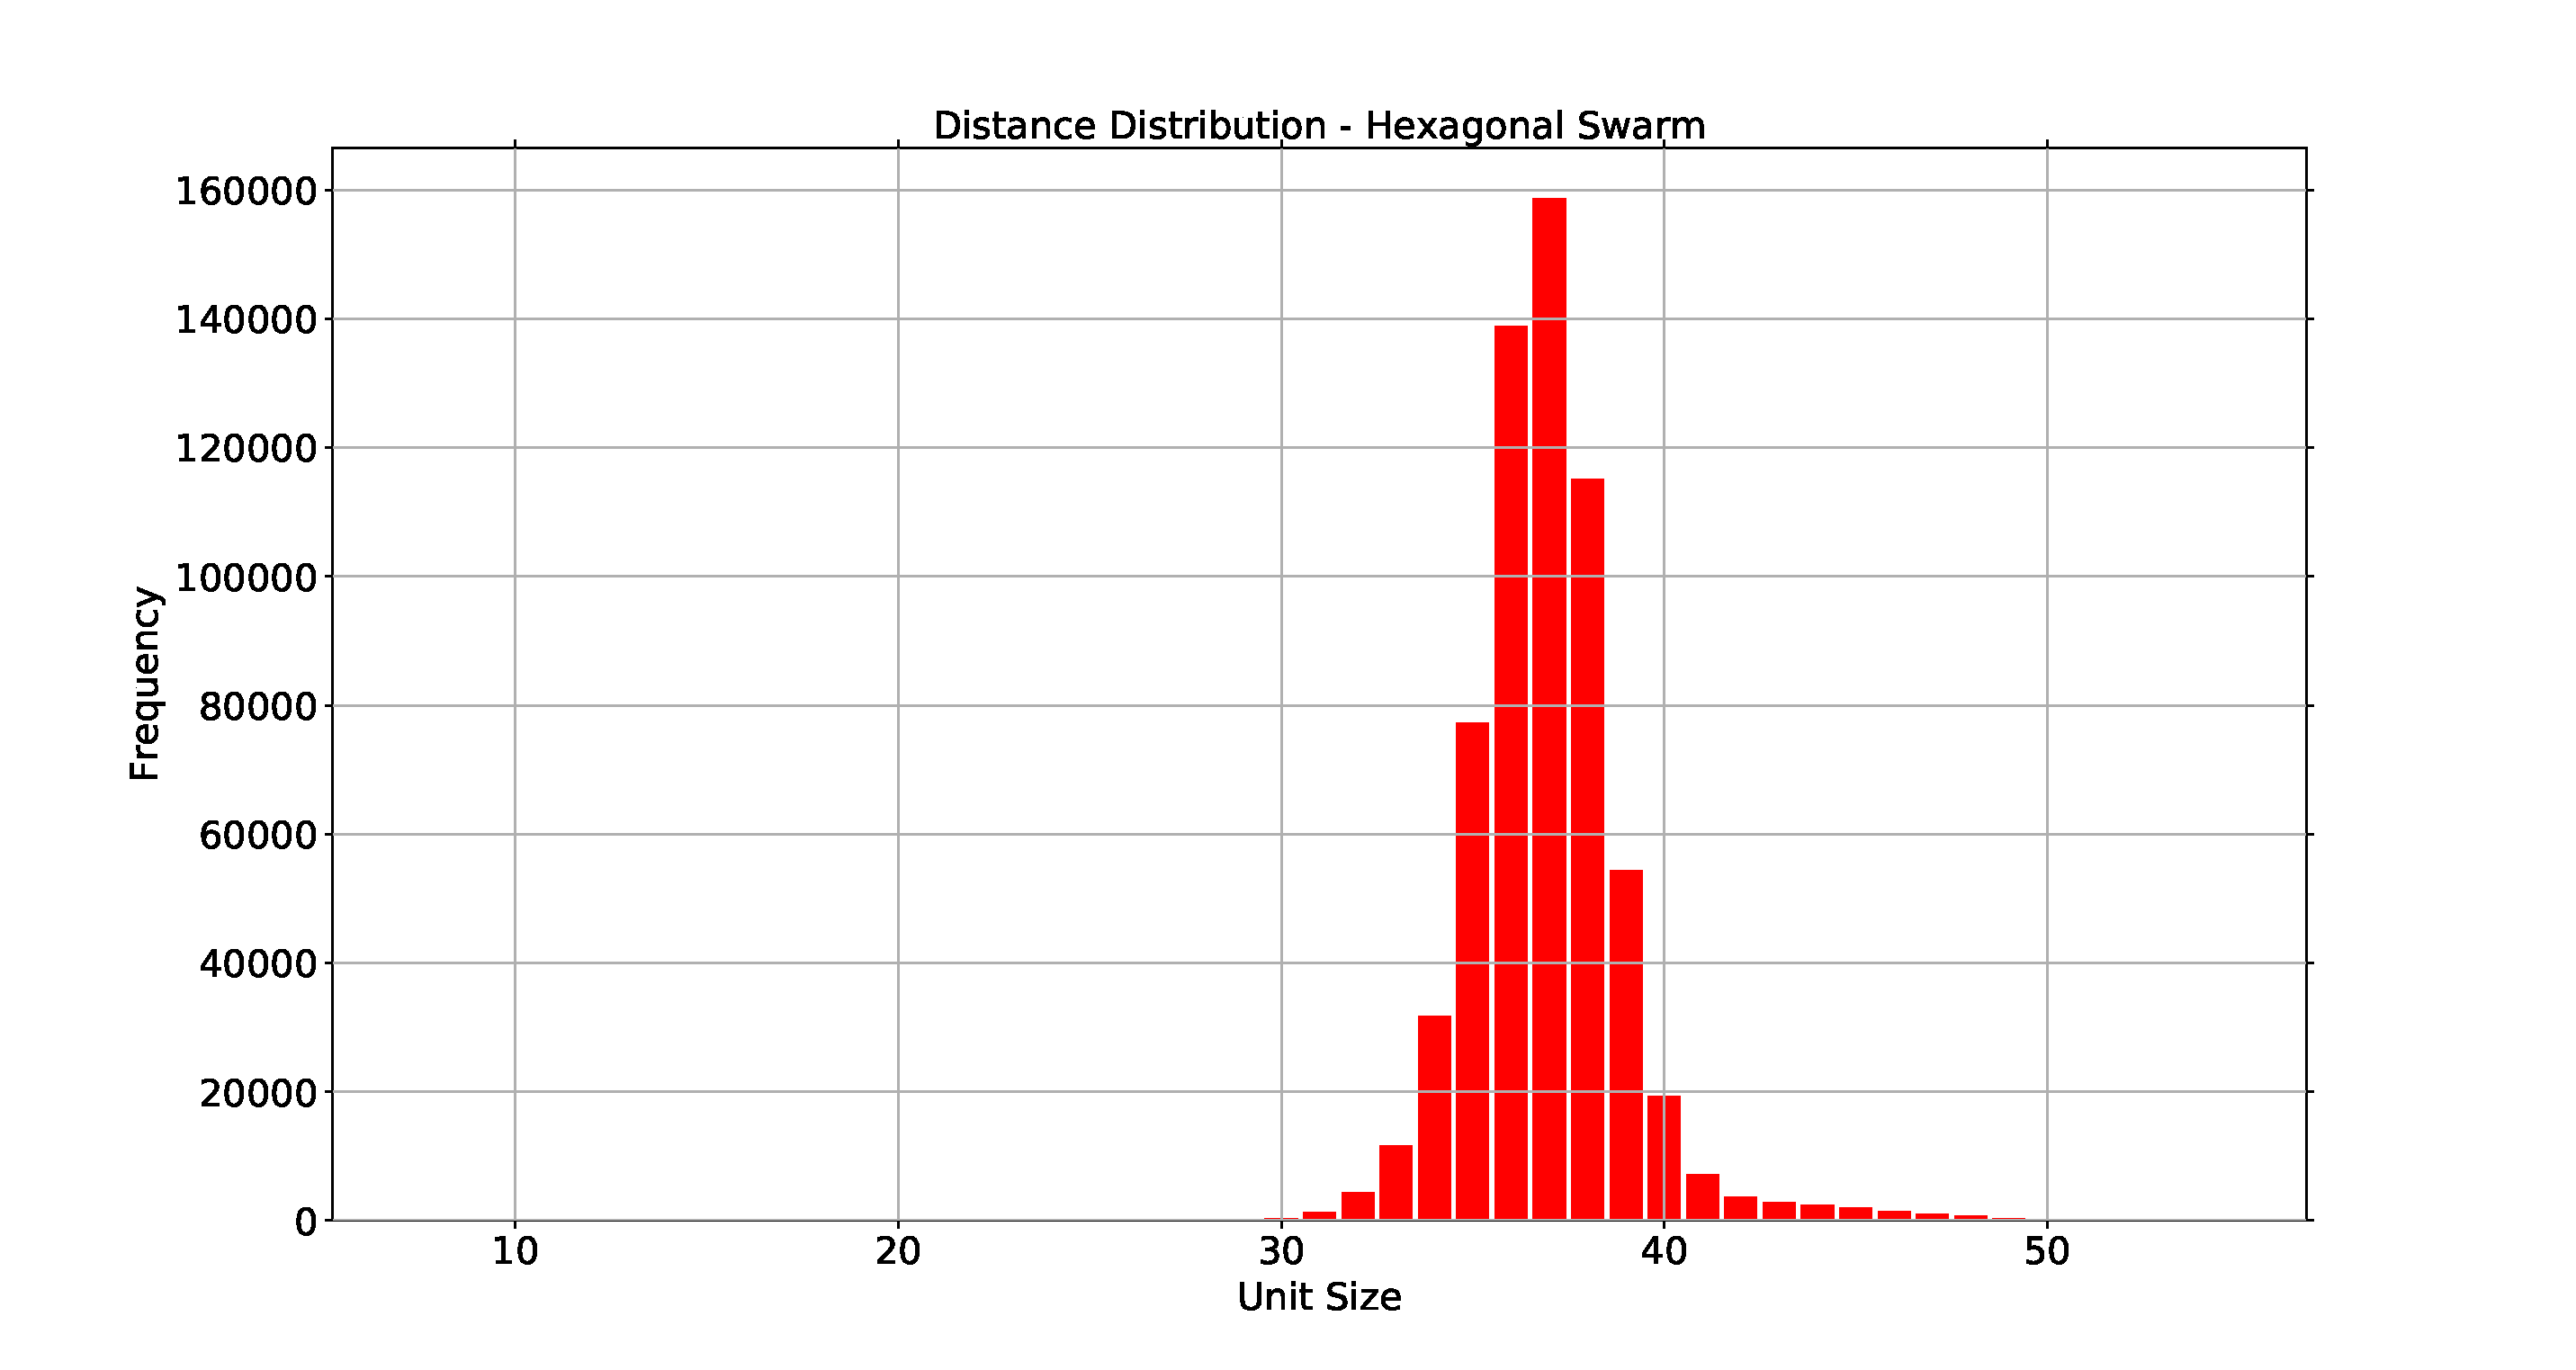
\includegraphics[width=13cm]{CHAPTER-5/figures/StabilityDistibutionHexagonal}
\end{center}
\caption{Distance distribution\label{methods:StabilityDistributionHexagonal}}
\end{figure}

Figures~\ref{methods:StabilityDistributionHexagonal3D} and \ref{methods:StabilityDistributionHexagonal3D2} show the distributions at each time cycle and shows the changes in the distribution of the distances as the agents coalesce into a stable structure. \autoref{methods:StabilityDistributionHexagonal3D} shows the initial distribution for the time intervals from 0 to 100 cycles (10 seconds). As the cycles progress the mean increases and the standard deviation reduces as the inter-agent distances equalise. \autoref{methods:StabilityDistributionHexagonal3D2} shows the final state of the swarm after 10 seconds.
%HEX-DIST-BAR-3D.py
\begin{figure}[H]
%\begin{center}
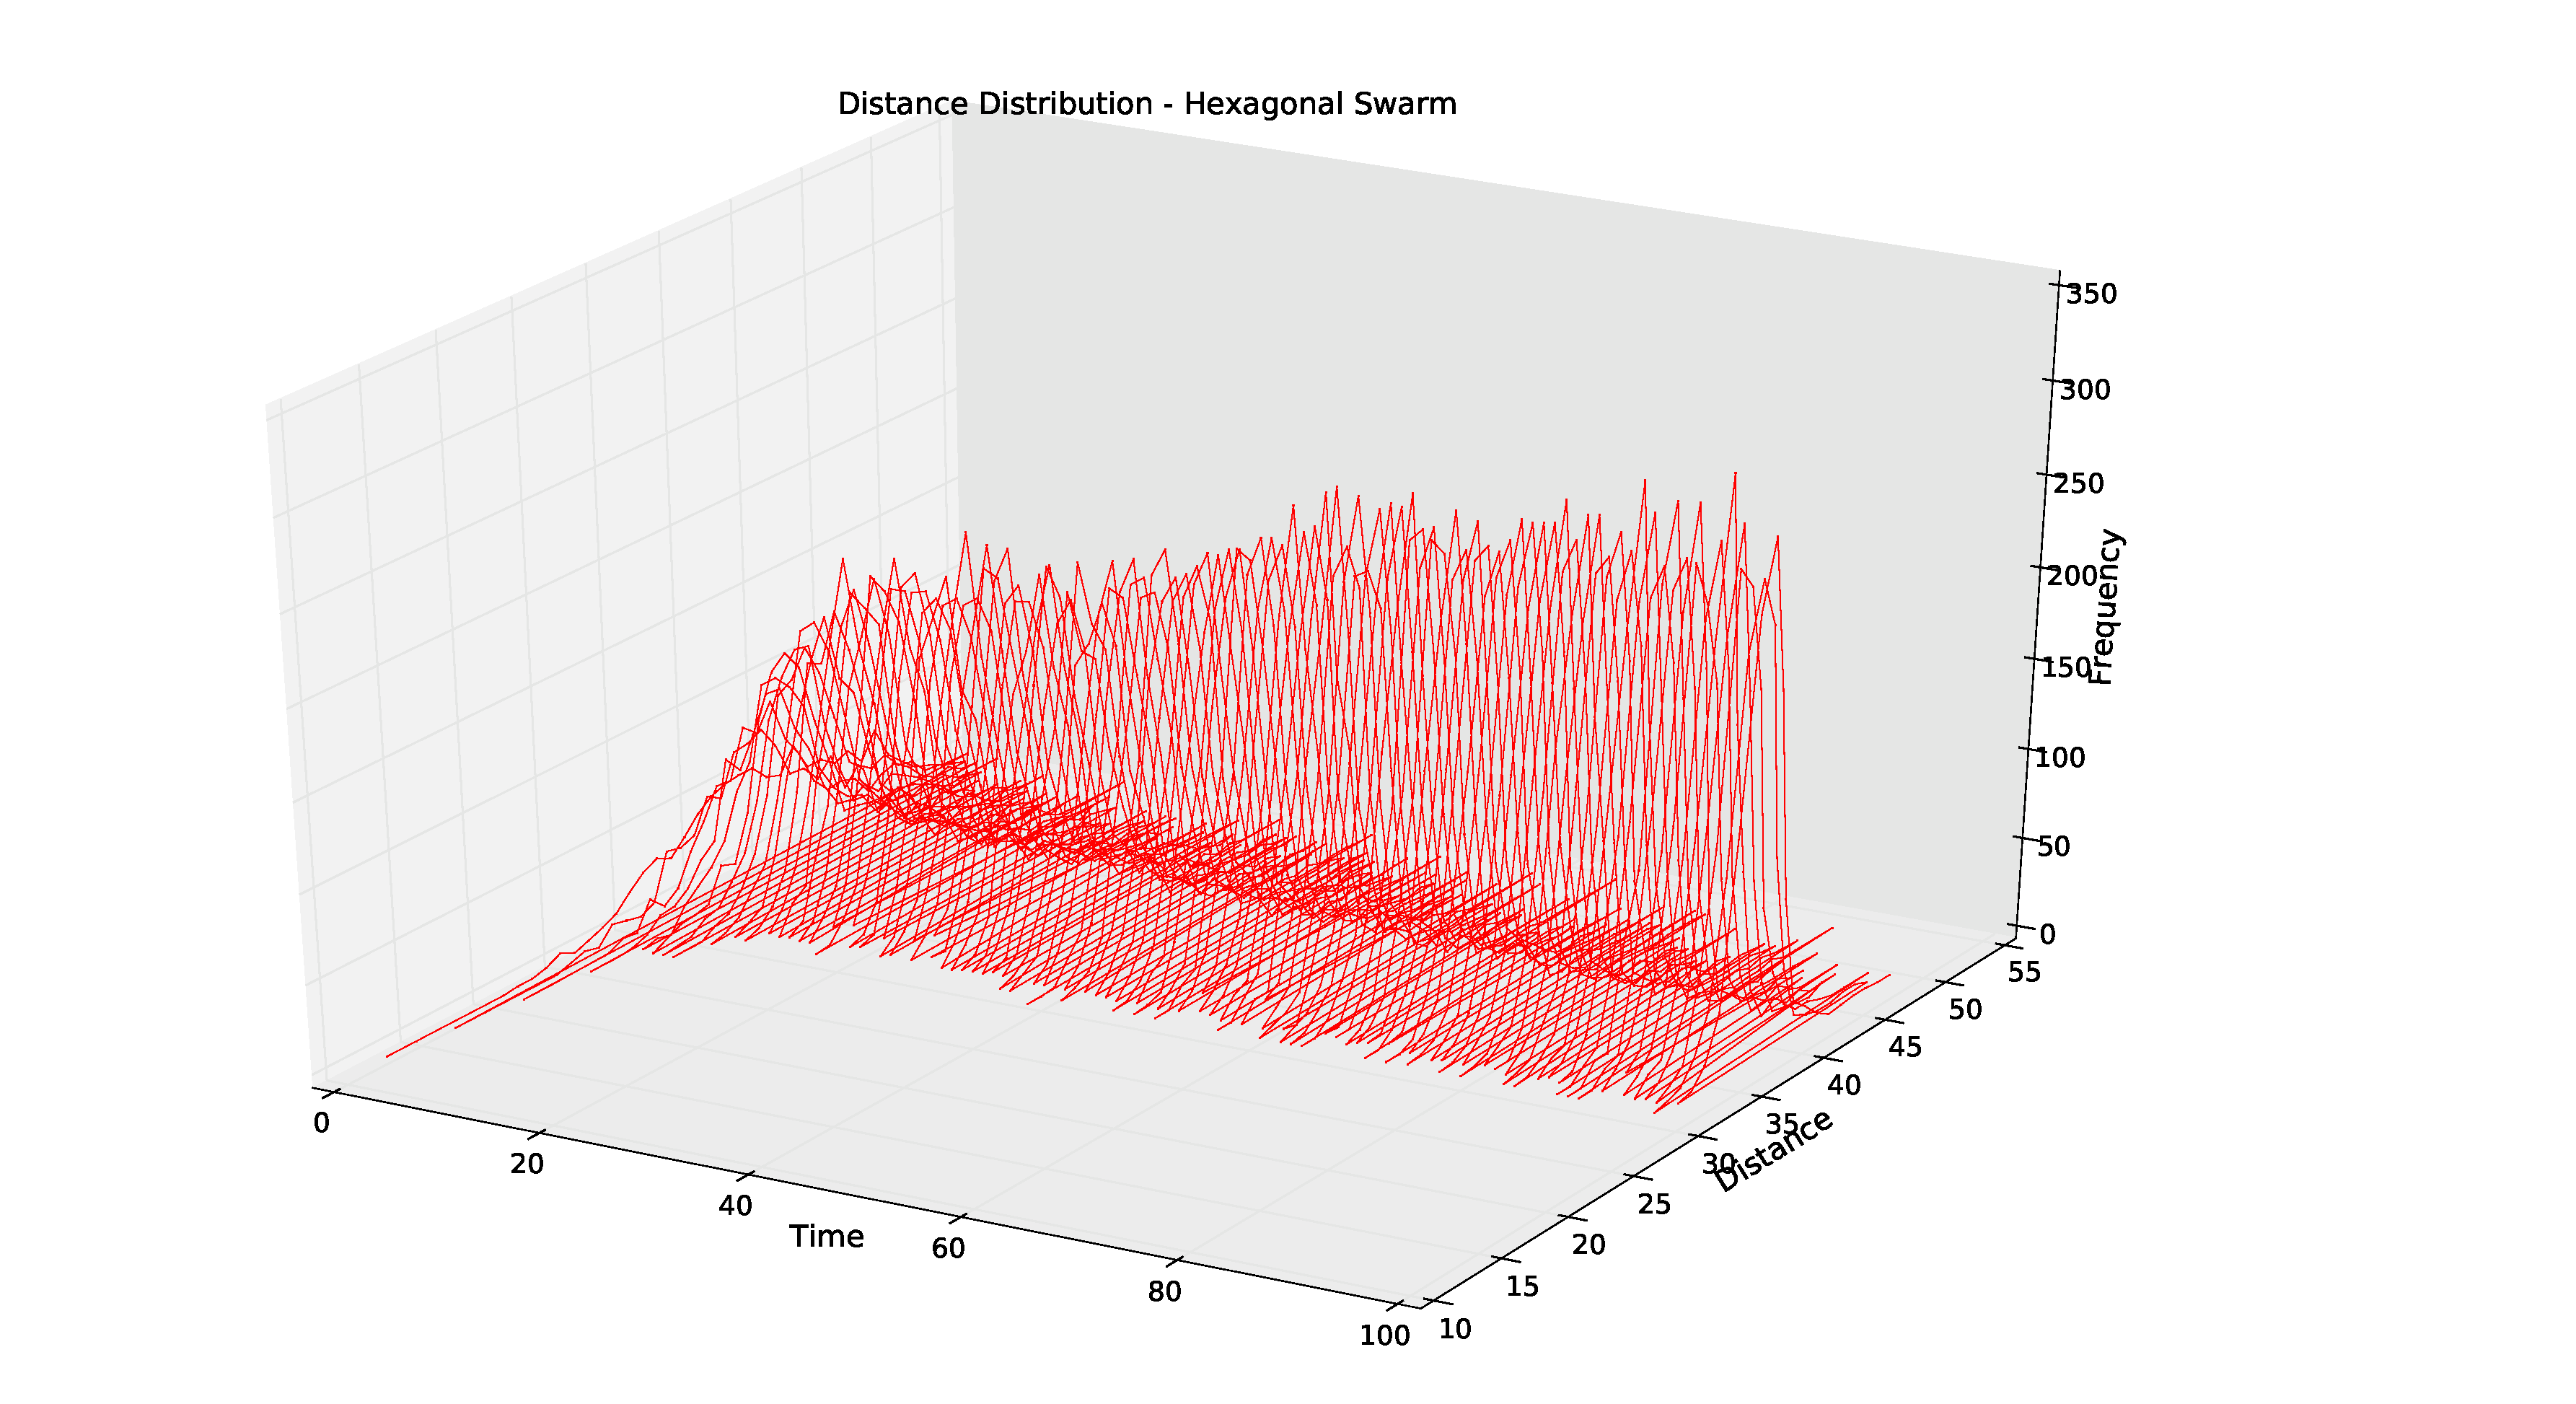
\includegraphics[width=15cm]{CHAPTER-5/figures/StabilityDistibutionHexagonal3D}
%\end{center}
\caption{Distance distribution / Time 0-10 seconds\label{methods:StabilityDistributionHexagonal3D}}
\end{figure}

\begin{figure}[H]
%\begin{center}
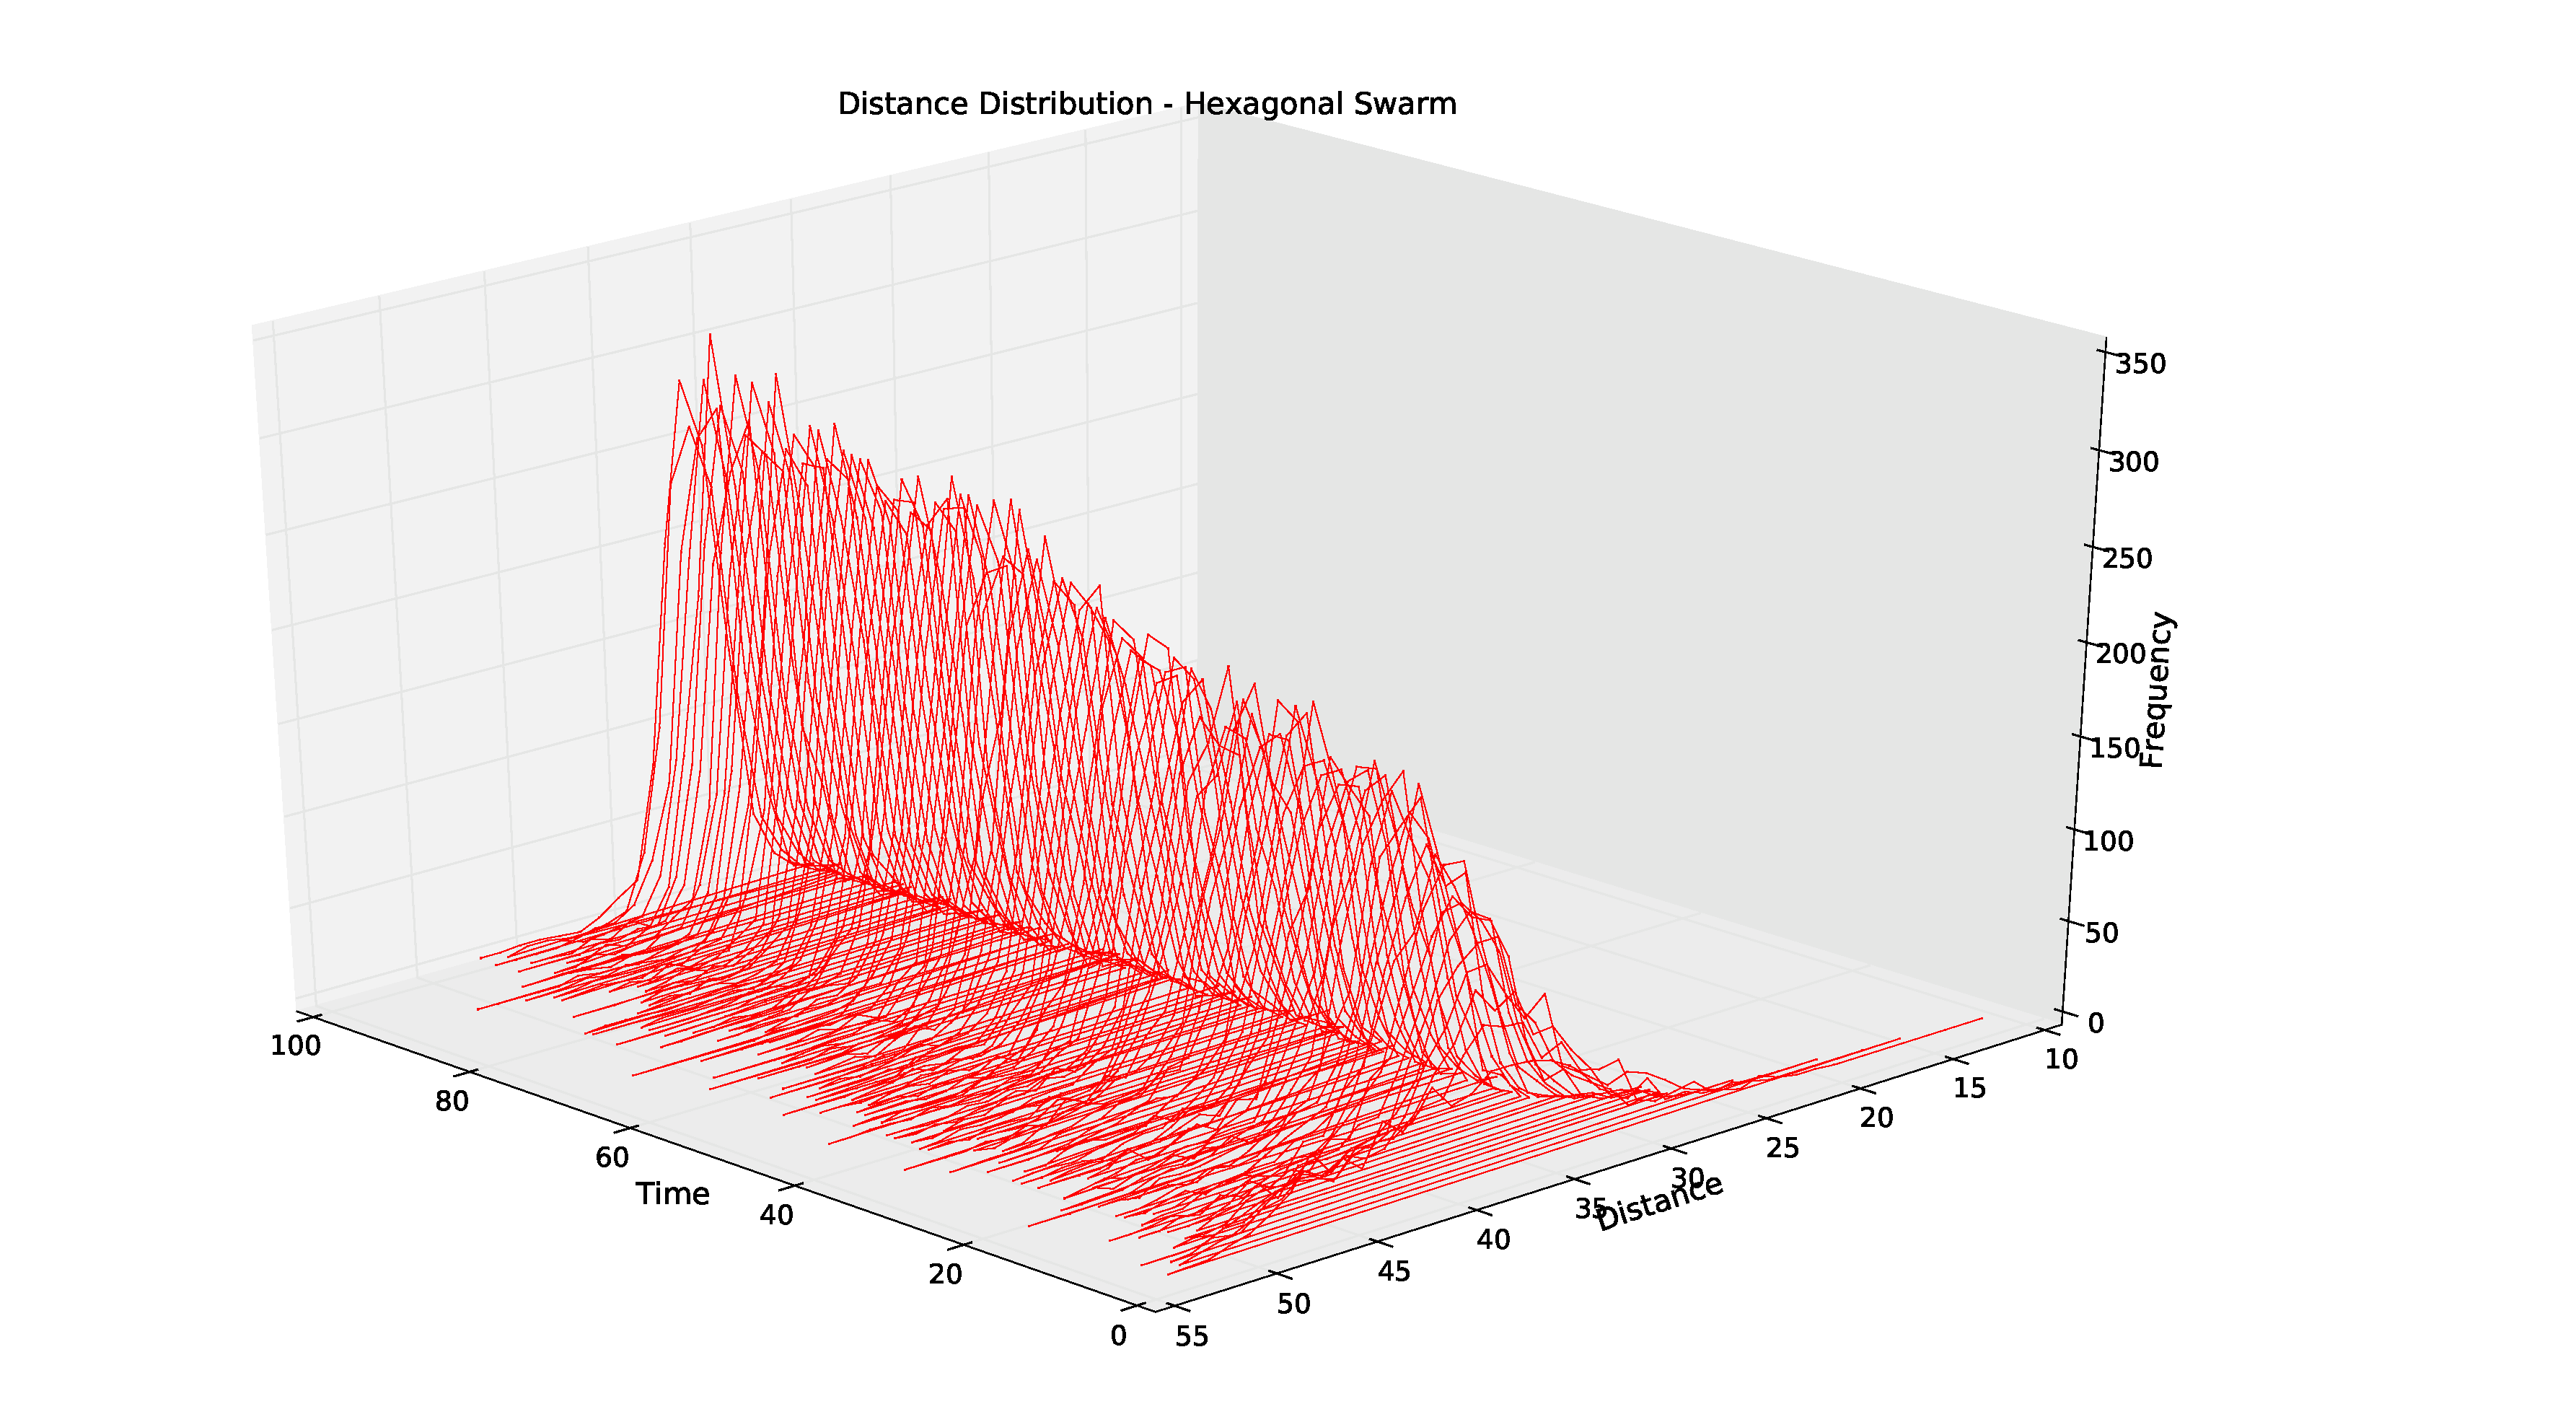
\includegraphics[width=15cm]{CHAPTER-5/figures/StabilityDistibutionHexagonal3D2}
%\end{center}
\caption{Distance distribution / Time 10-0 seconds\label{methods:StabilityDistributionHexagonal3D2}}
\end{figure}

\subsection[Agent resultant magnitude based metric]{Agent resultant magnitude (\textit{interaction vector}) based metric}
The distribution of the \textit{interaction vector} magnitude can be plotted in the same manner as the distances. \autoref{methods:StabilityMagnitudeHexagonal} shows the distribution of the agents based on the \textit{interaction vector} magnitude for the entire duration of the simulation. As with the distance based metric the data forms a normal bell shaped distribution with a mean magnitude evolving in time as shown in \autoref{methods:StabilityMagnitudeSwarm40-50}. \autoref{methods:StabilityMagnitudeHexagonal} includes negative magnitudes, this indicates that sections of the swarm are expanding. 
%HEX-MAG.py
\begin{figure}[H]
\begin{center}
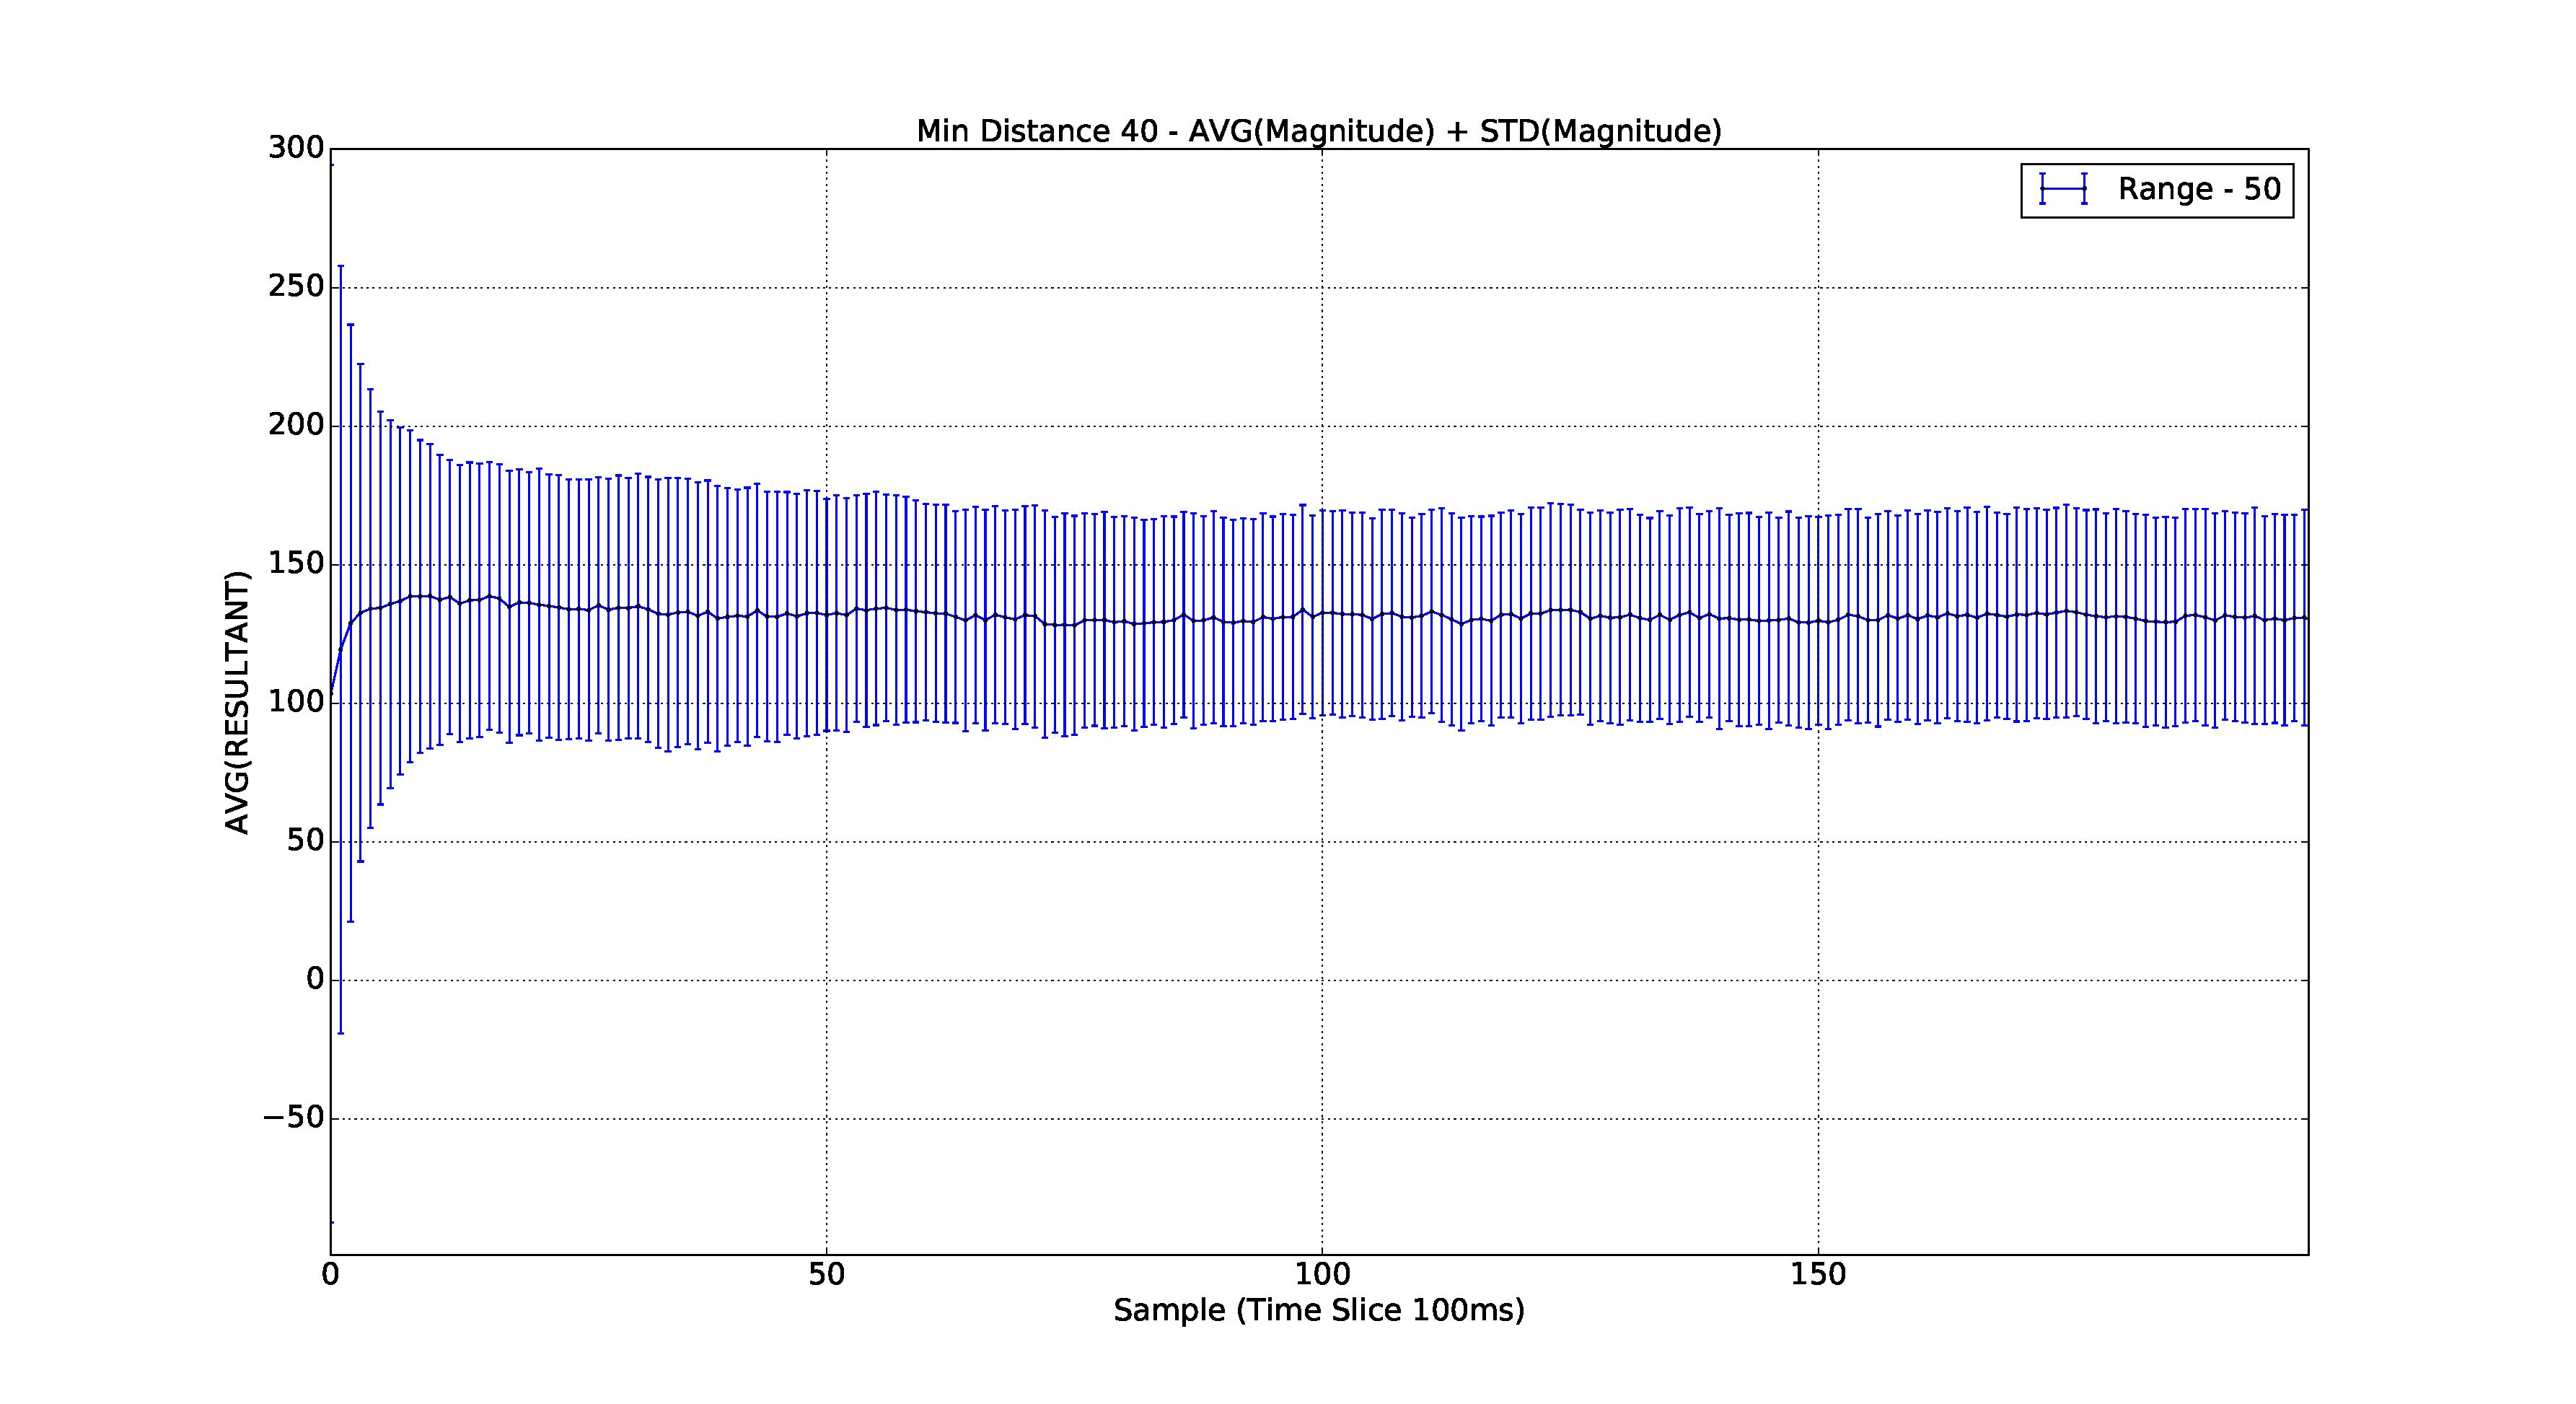
\includegraphics[width=13cm]{CHAPTER-5/figures/StabilityMagnitudeSwarm40-50}
\end{center}
\caption{Hexagonal swarm - Agent resultant magnitude metric\label{methods:StabilityMagnitudeSwarm40-50}}
\end{figure}
%HEX-MAG-BAR.py
\begin{figure}[H]
\begin{center}
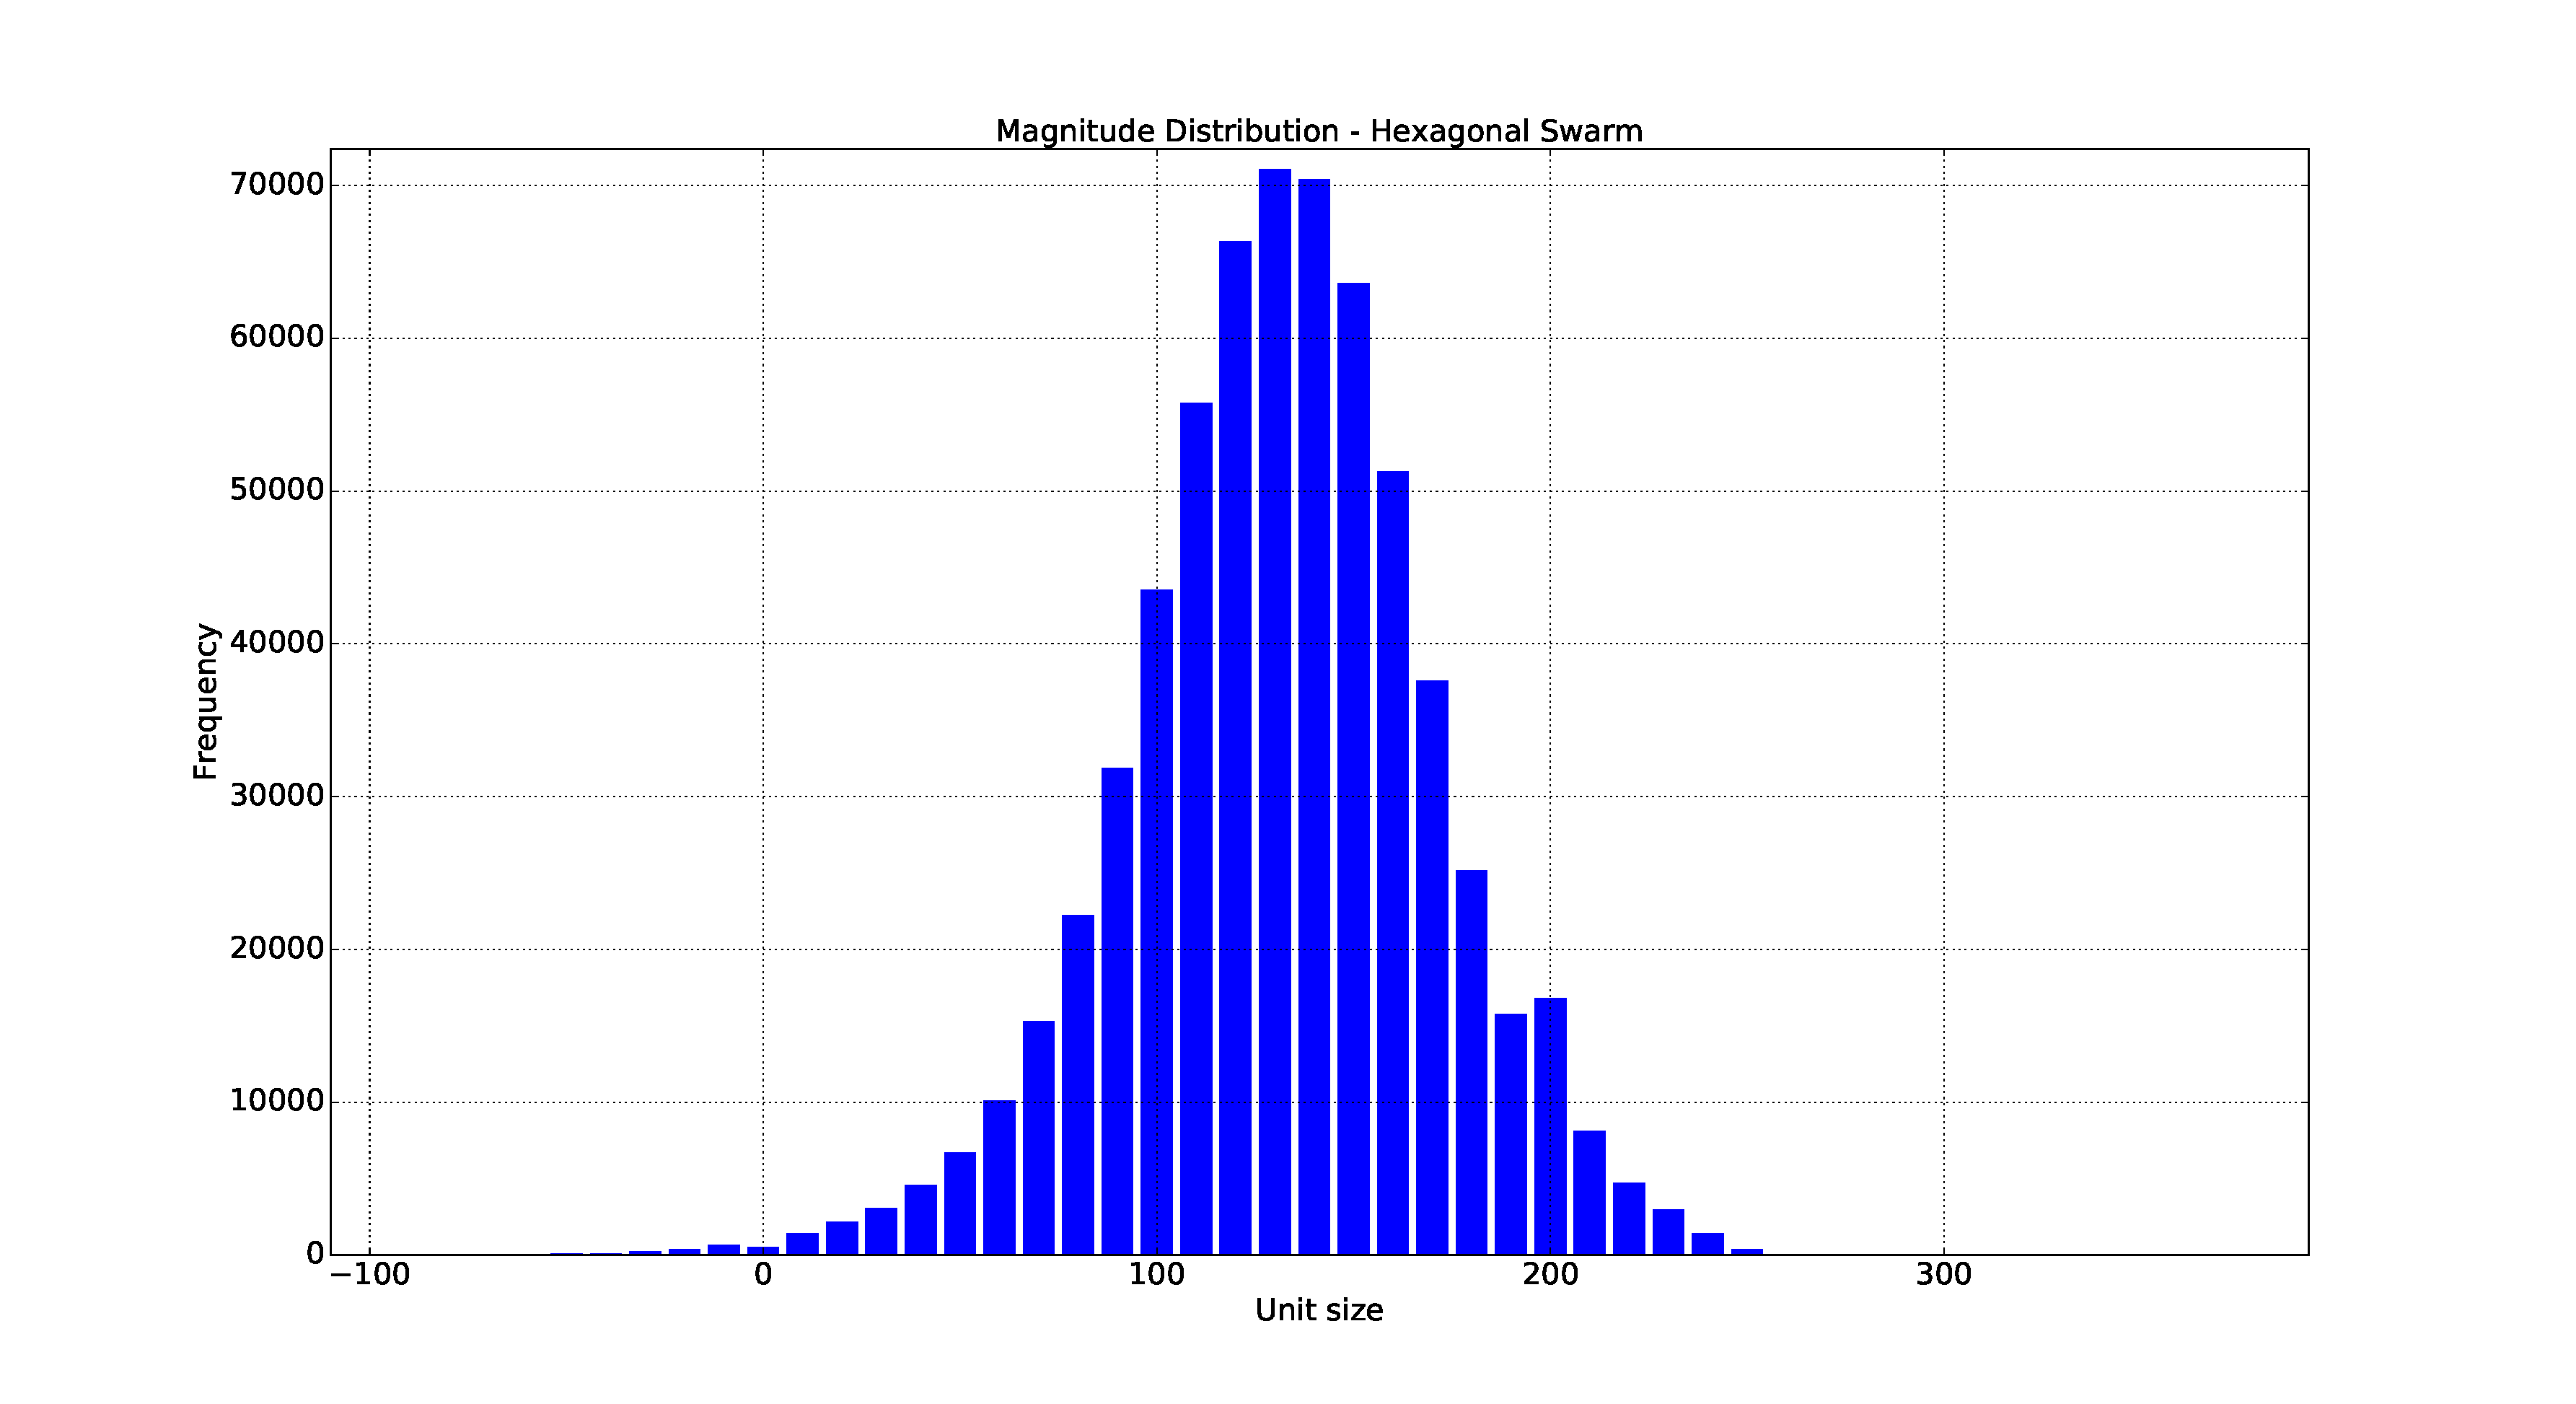
\includegraphics[width=13cm]{CHAPTER-5/figures/StabilityMagnitudeHexagonal}
\end{center}
\caption{Agent resultant magnitude distribution\label{methods:StabilityMagnitudeHexagonal}}
\end{figure}

\autoref{methods:StabilityMagHexagonal3D} and \ref{methods:StabilityDistributionHexagonal3D2} show the distributions at each time cycle and show the change in the distributions of the magnitudes. As with the distance graphs \autoref{methods:StabilityMagHexagonal3D} shows the distribution at time interval 0 to 100 and \autoref{methods:StabilityMagHexagonal3D2} shows the final state of the swarm after 10 seconds (100 cycles).

\begin{figure}[H]
\begin{center}
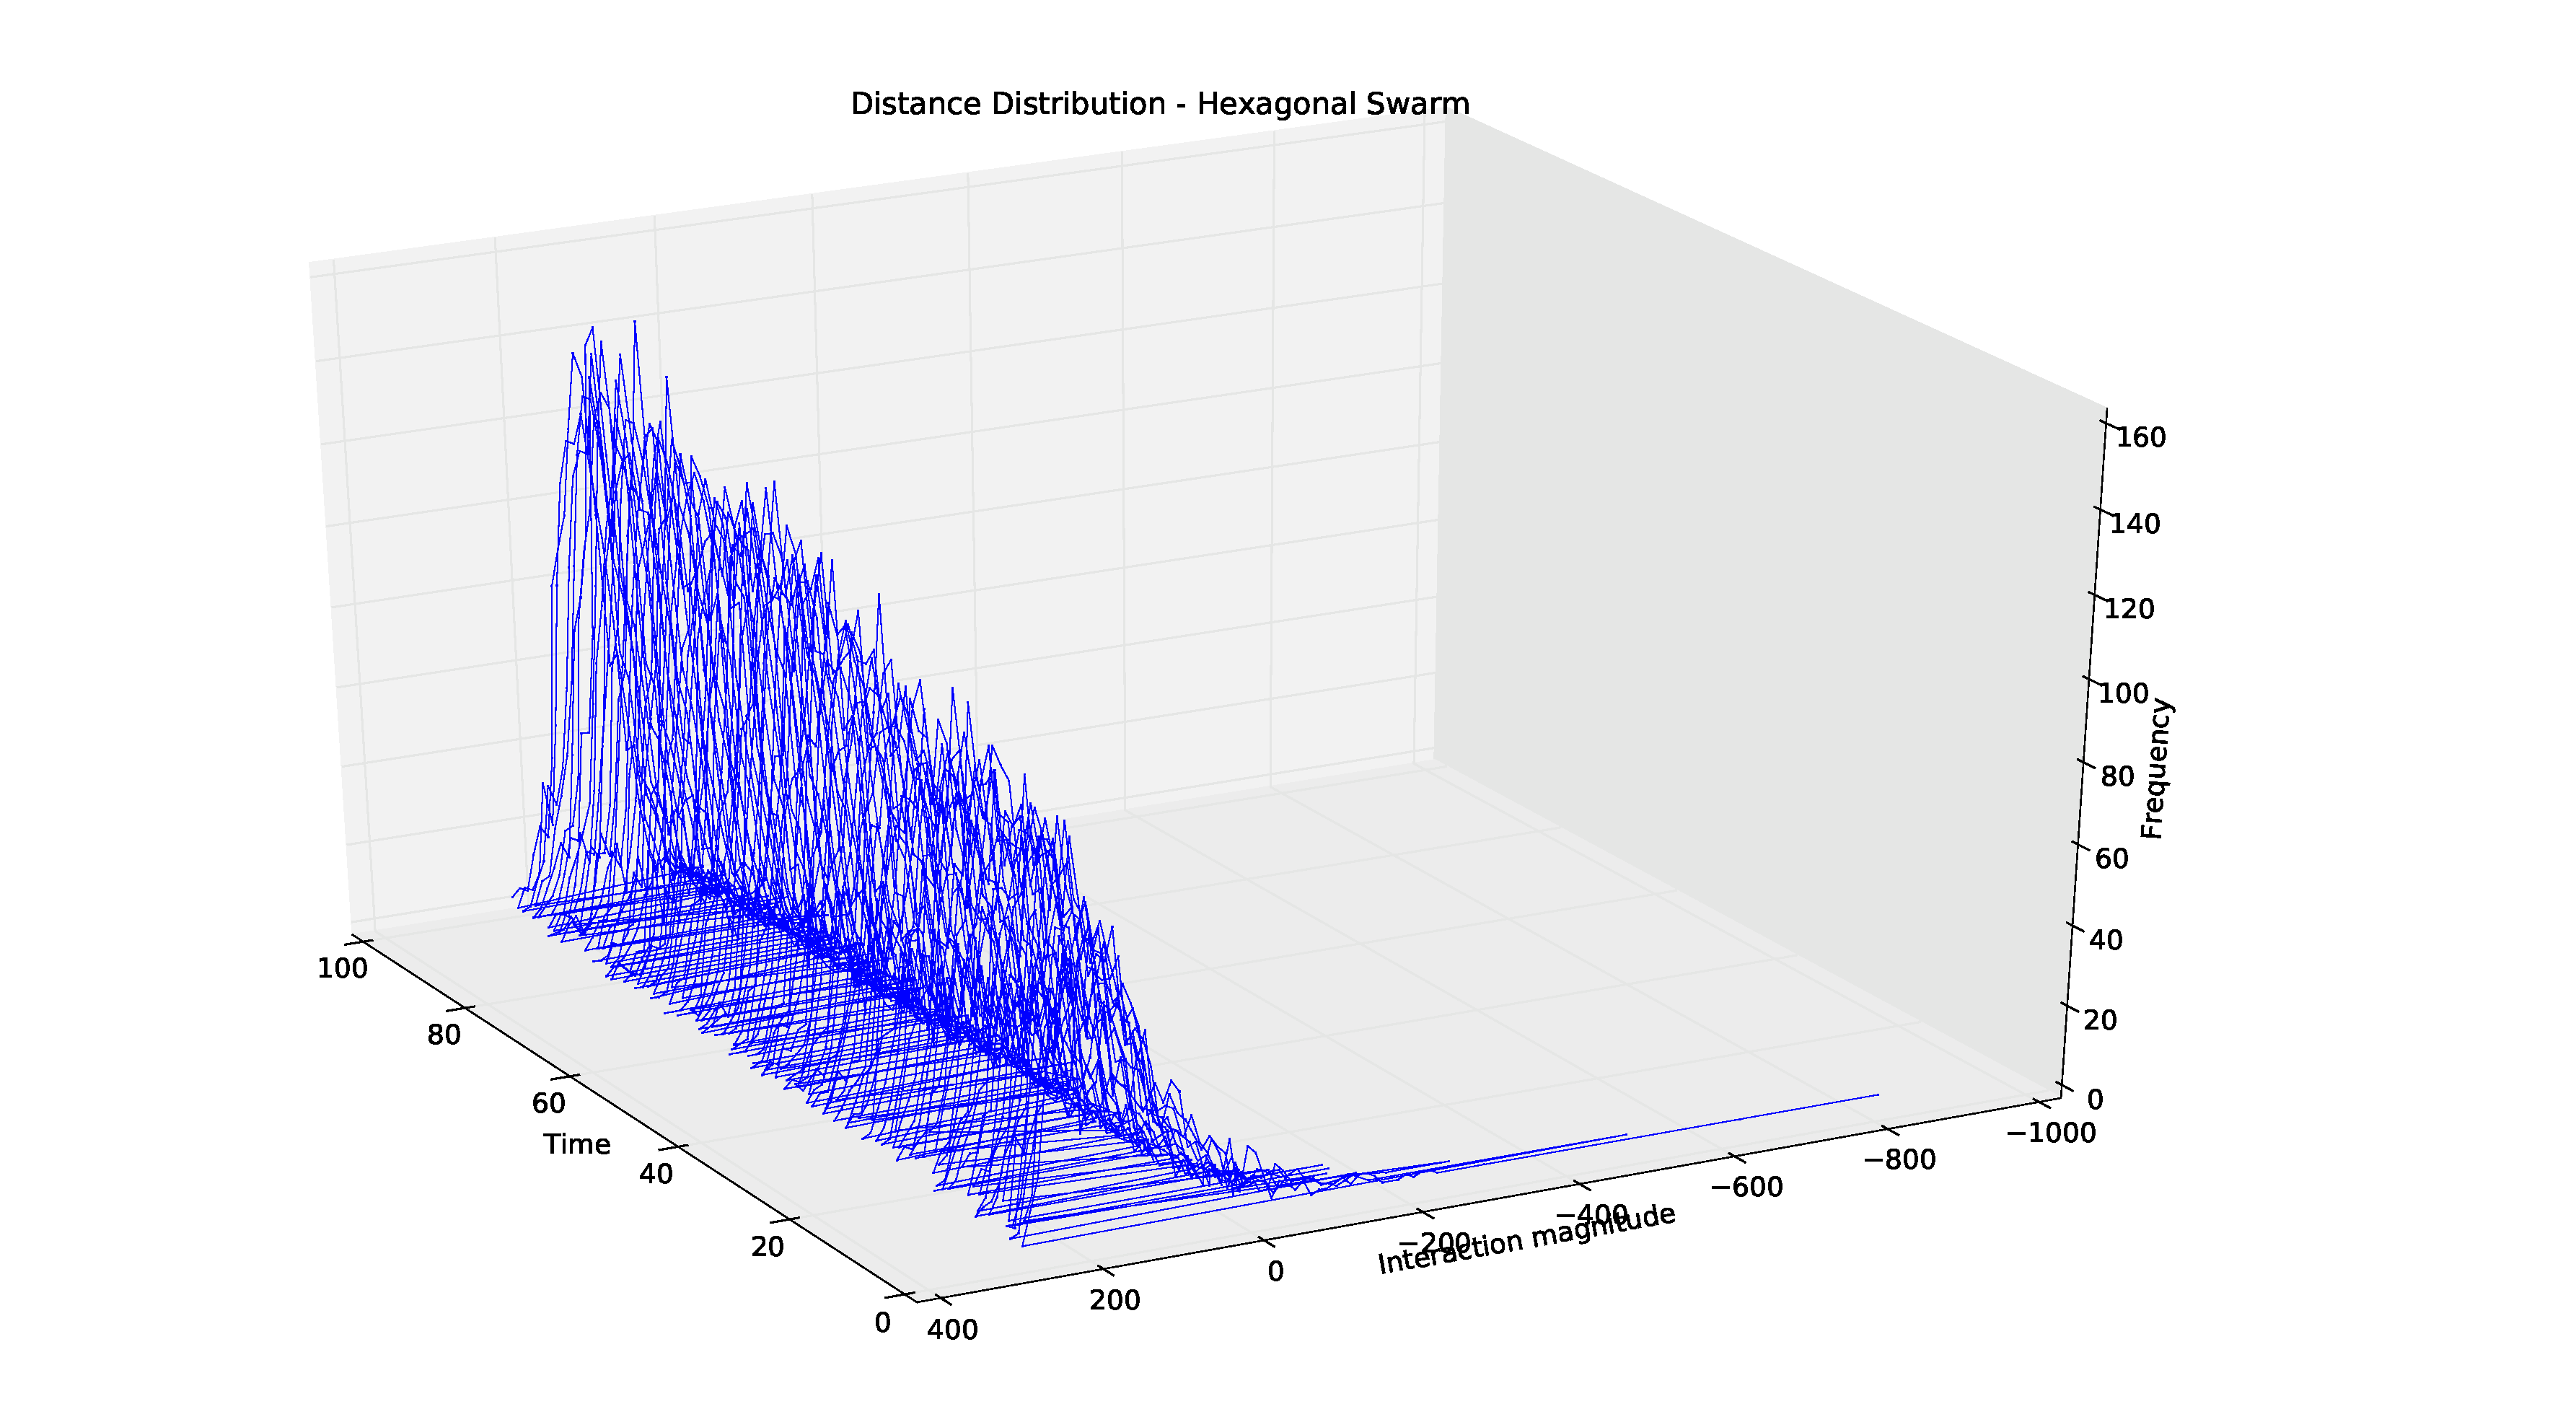
\includegraphics[width=13cm]{CHAPTER-5/figures/StabilityMagHexagonal3D}
\end{center}
\caption{Agent resultant magnitude distribution / Time 0-10 seconds\label{methods:StabilityMagHexagonal3D}}
\end{figure}

\begin{figure}[H]
\begin{center}
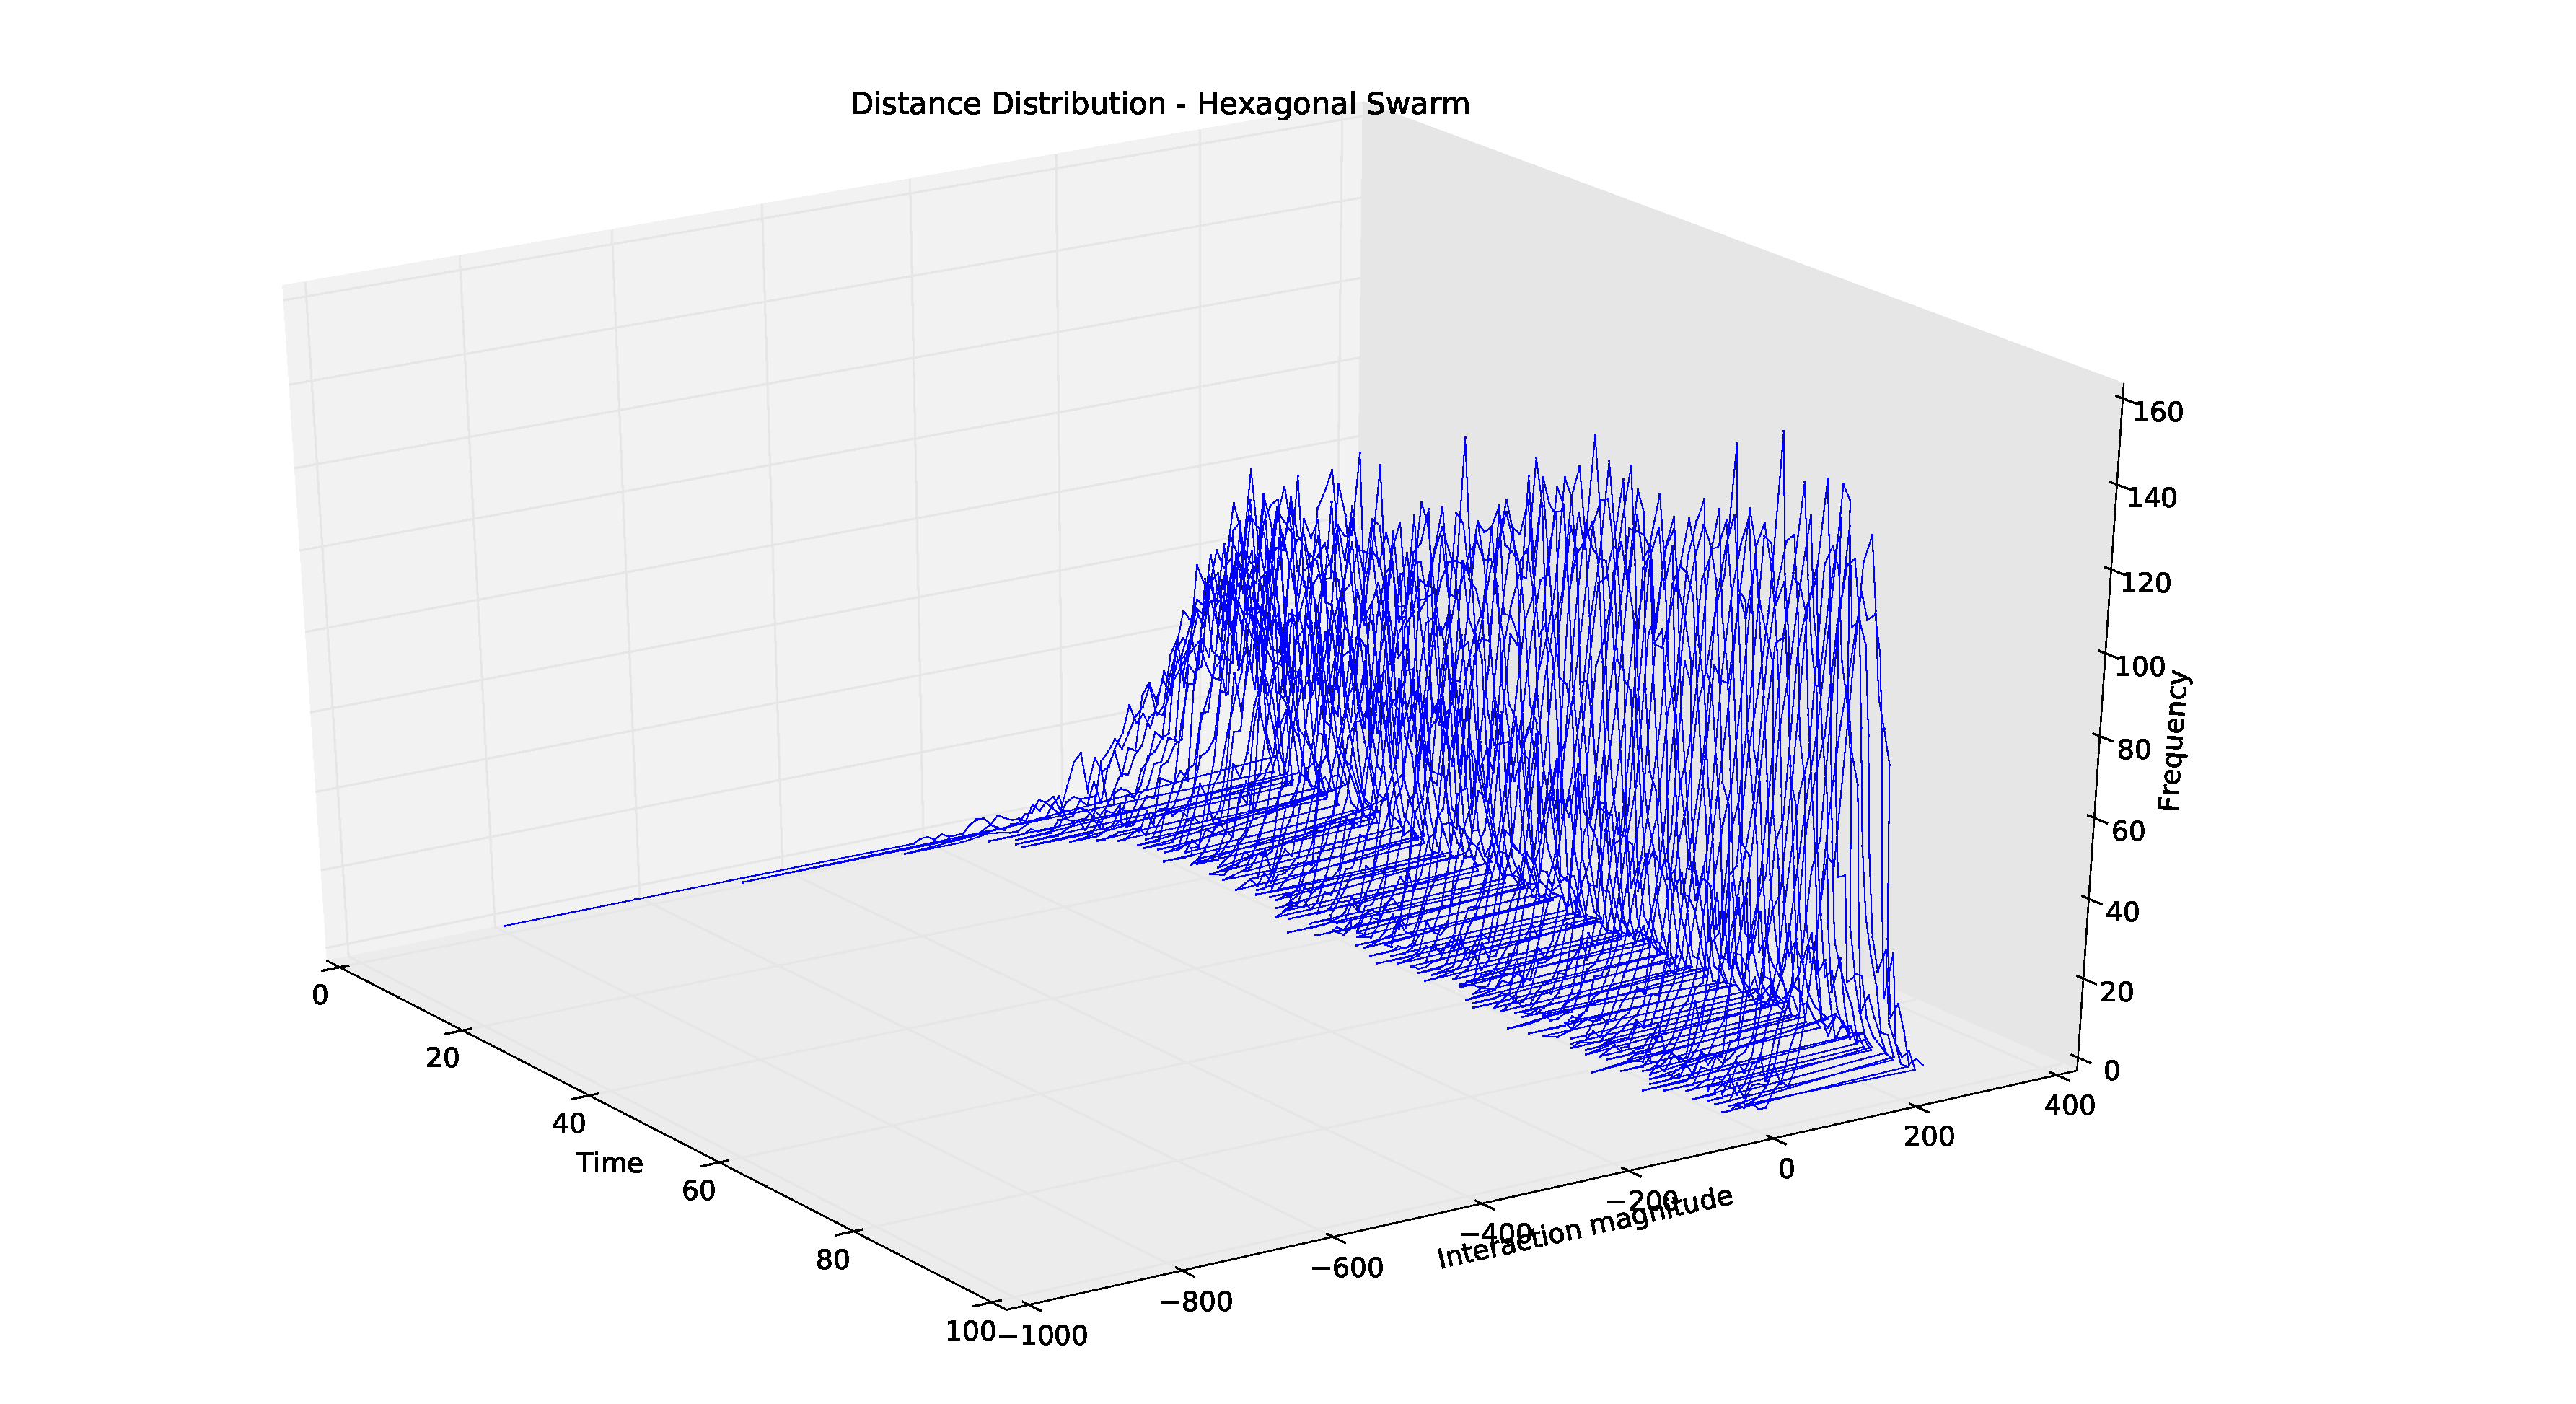
\includegraphics[width=13cm]{CHAPTER-5/figures/StabilityMagHexagonal3D2}
\end{center}
\caption{Agent resultant magnitude distribution / Time 10-0 seconds\label{methods:StabilityMagHexagonal3D2}}
\end{figure}

The hexagonal structure is the most stable structure \cite{HT:2001} and can be classed as a swarm's most efficient state as the swarm is maximally distributed with agents having minimal or no cross connected agents. These results show that the field effects are producing a swarm that will tend towards having all distances equal which will produce the hexagonal effect as shown in \autoref{fig:StableForms} on page \pageref{fig:StableForms}.

\section{Hyper-connected swarm analysis}\label{section:AnalysisB}
When the field effects create a hyper-connected swarm the inter connectivity of the agents create a multi-modal distribution of the inter-agent distances. \autoref{methods:CrushedStability1} shows the inter-agent distances highlighted, near neighbours in green and extended neighbours in red. This is detectable in terms of how the internal movement metrics present these distributions. A hyper-connected swarm has a high level of cohesion causing the swarm to become very inflexible. The swarm appears `stable' in terms how the overall structure is maintained~(\autoref{methods:StableSwarmCompressed}), however, there is a greater variation in the \textit{interaction vector} magnitudes, and resultant distances, than in a hexagonal swarm. The distances will maintain a good sound structure but the standard deviation from the mean is high. This elevated standard deviation~(\autoref{methods:StabilityDistanceSwarm40-60} and ~\ref{methods:StabilityMagnitude40-60}) indicates that the swarm is not at its optimum distribution as the swarm's agents could be distributed further covering a greater area without causing the swarm to break up. This can be achieved by increasing the repulsion field effect. In some circumstances this hyper-connected structure may be a desirable configuration to create a more `rigid' platform: for instance to provide a close proximity wireless sensor network with multiple routing pathways. The connected distribution that causes the high standard deviation can be seen in \autoref{methods:StabilityDistributionHyper}. There are two distinct peaks in the inter-agent distribution at approximately 38 and 58 units

\begin{figure}[H]
\begin{center}
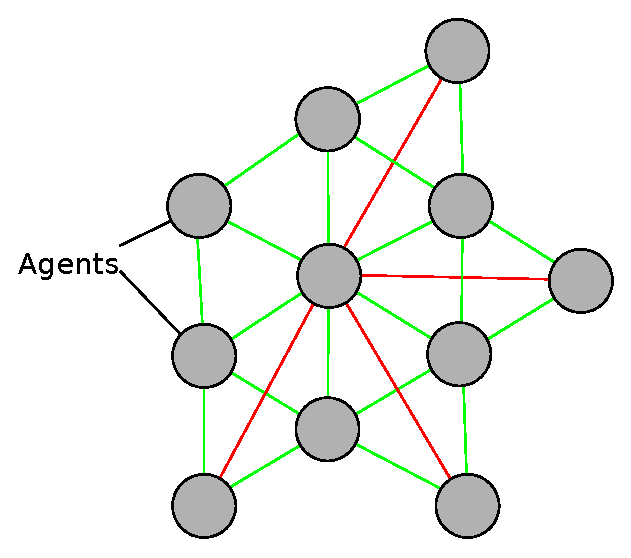
\includegraphics[width=7cm]{CHAPTER-5/figures/CrushedStability}
\end{center}
\caption{Inter-agent links in a hyper-connected swarm} \label{methods:CrushedStability1}
\end{figure}

\begin{figure}[H]
\begin{center}
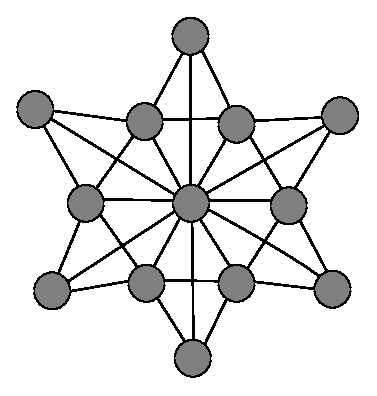
\includegraphics[width=6cm]{CHAPTER-5/figures/StableFormsCompressed}
\end{center}
\caption{Hyper-connected structure} \label{methods:StableSwarmCompressed}
\end{figure}

\subsection{Distance based metric}
The distance based analysis graph~(\autoref{methods:StabilityDistanceSwarm40-60}) for the hyper-connected swarm shows the metrics being applied to the swarm over a period of 200 cycles. 

The swarm is initially in a state of disorganisation and the average distance over the first 20 cycles shows the swarm compressing as the average distance falls. The swarm then enters a phase where the mesh structure forms and the swarm starts to stabilise. After about 100 cycles the field effects have resolved and the swarm structure settles to its most stable state for the given set of parameters. As with the hexagonal swarm the hyper-connected swarm's internal movement fluctuates to maintain the swarm's structure.
%HYPER.py
\begin{figure}[H]
\begin{center}
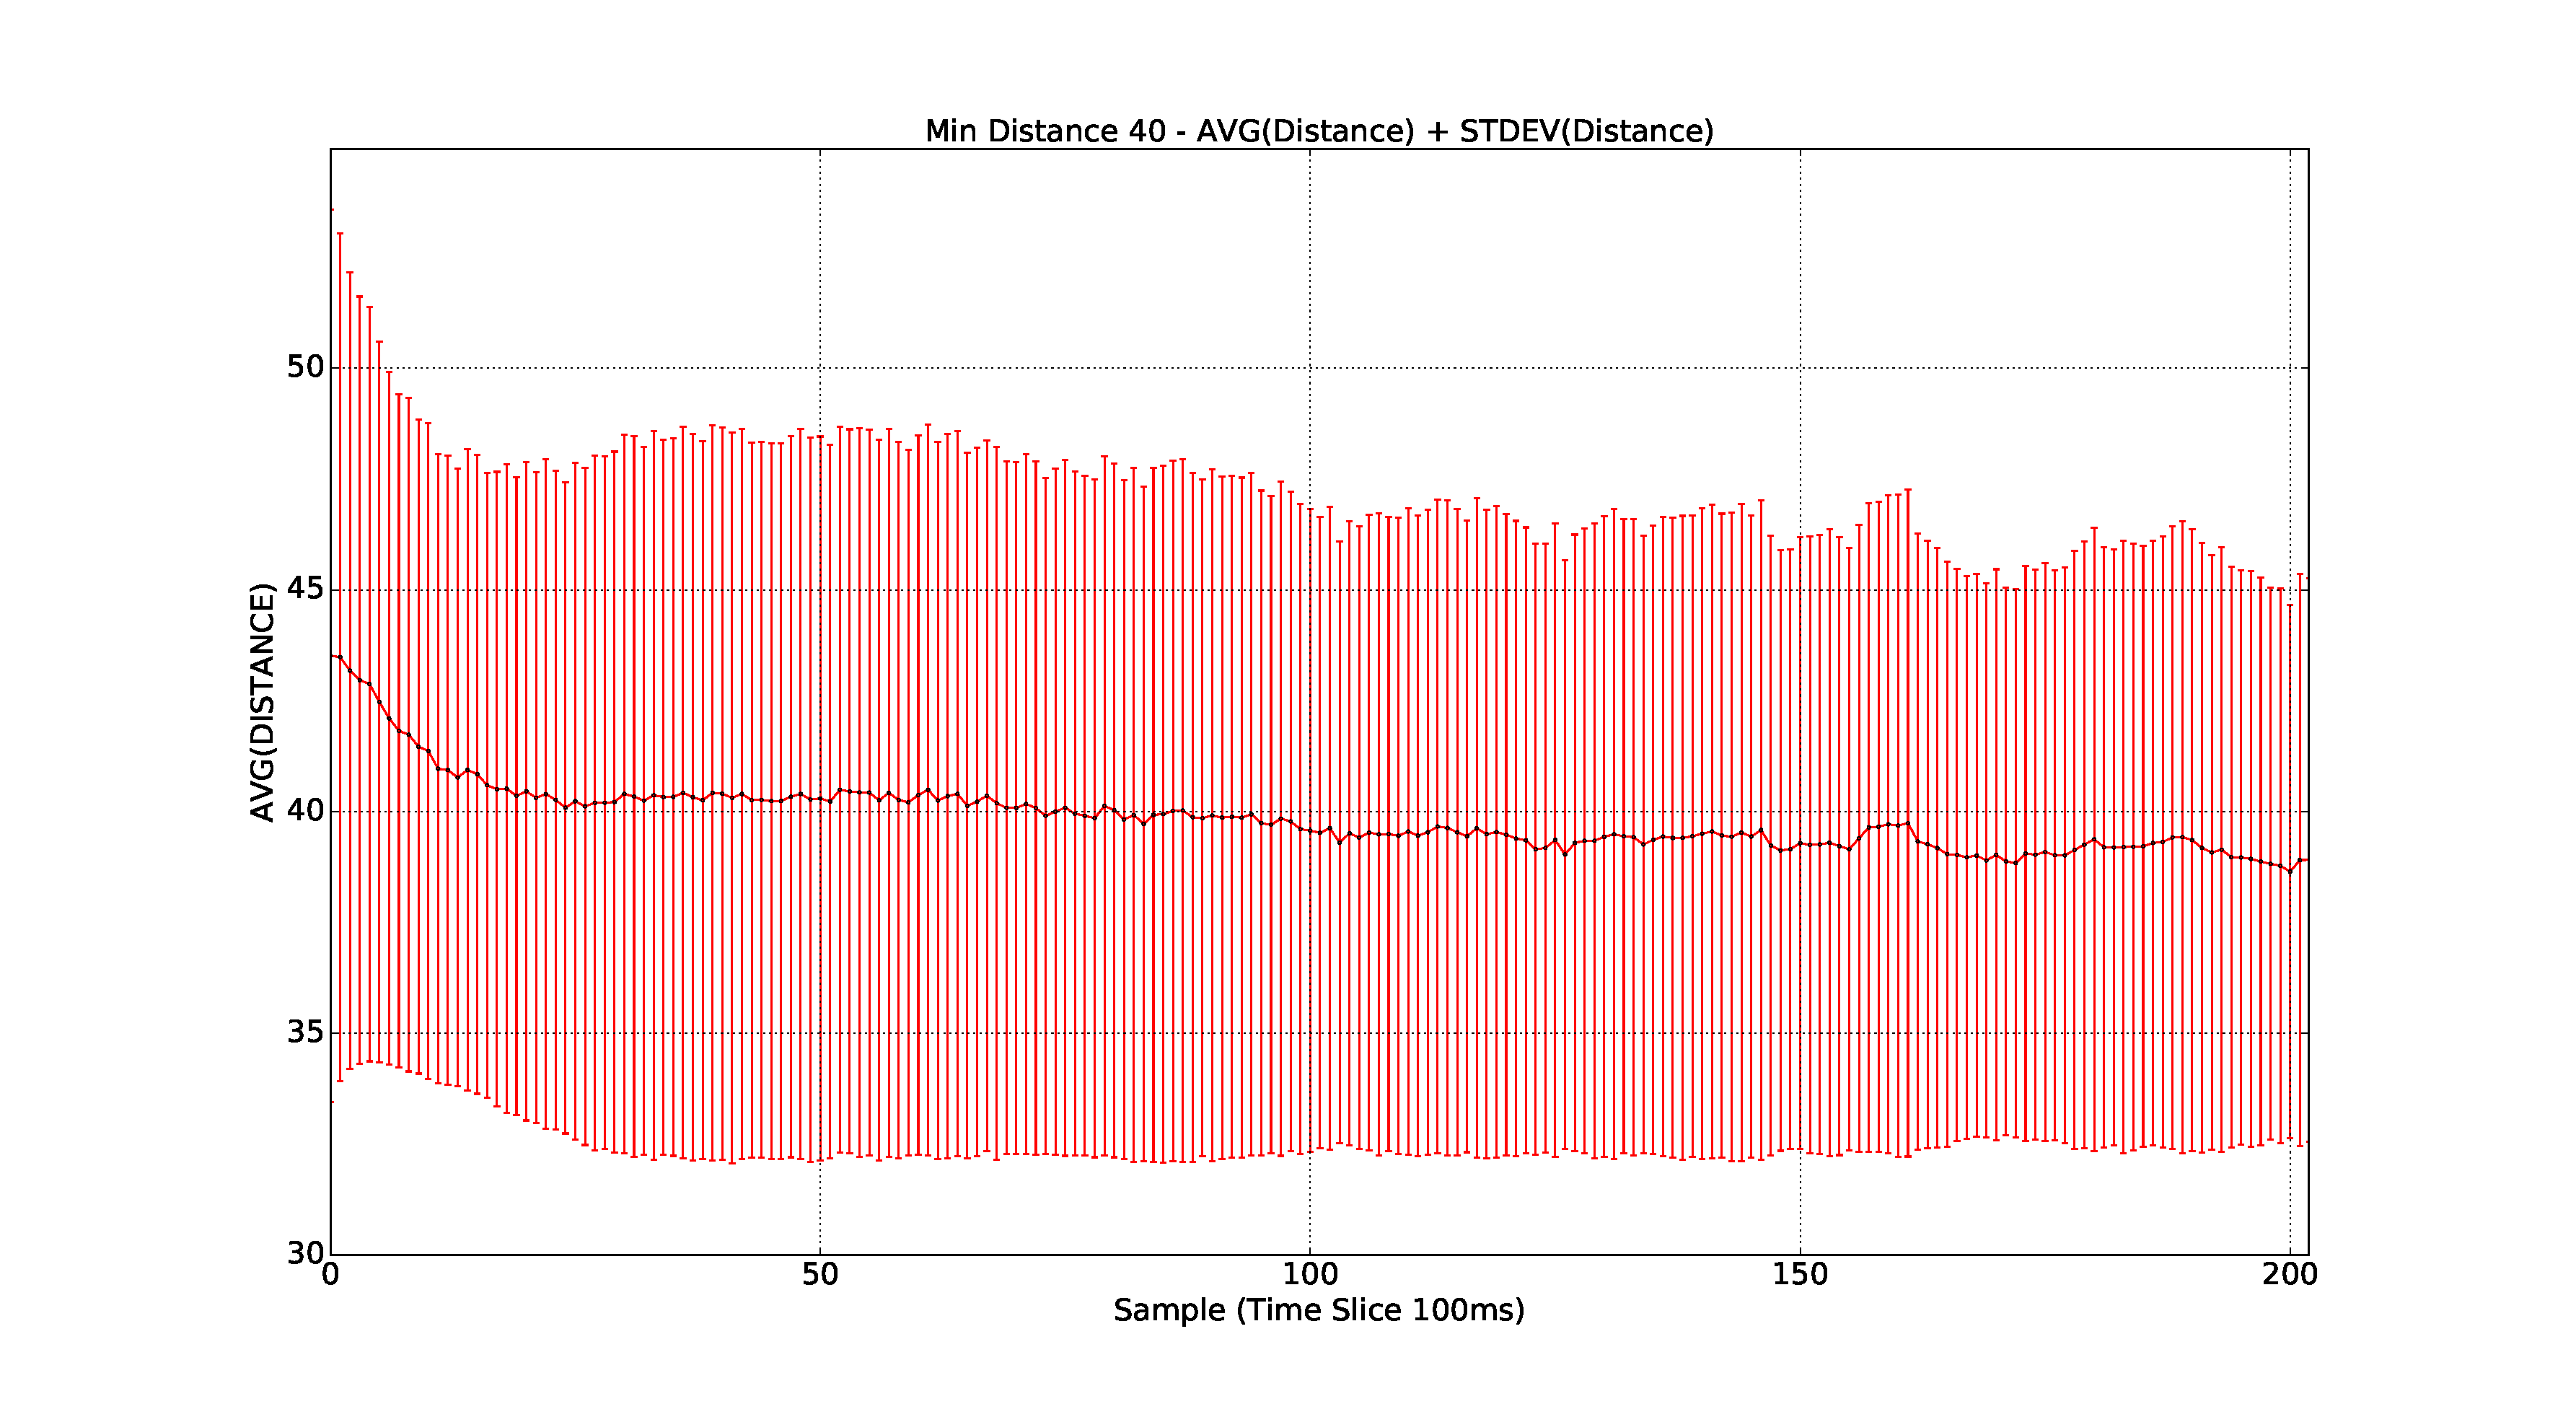
\includegraphics[width=13cm]{CHAPTER-5/figures/StabilityDistanceSwarm40-60}
\end{center}
\caption{Distance metric\label{methods:StabilityDistanceSwarm40-60}}
\end{figure}

\autoref{methods:StabilityDistributionHyper} shows the distribution of the agents over the entire simulation. By looking at the data in terms of the distribution graph it is possible to identify why the standard deviation is greater than that of the hexagonal swarm. The field effects, in this simulation, have created a bi-modal hyper-connected swarm. A bi-modal swarm is created when the agents in a swarm have the cohesion feild effect set such that agents are neighbours one level further out from the immediate neighbours as shown in Figure~\ref{methods:StableSwarmCompressed}. The result of this type of connectivity is that the distribution of the agents distances will produce two peaks in the distribution graph.

%HYPER-DIST-BAR.py
\begin{figure}[H]
\begin{center}
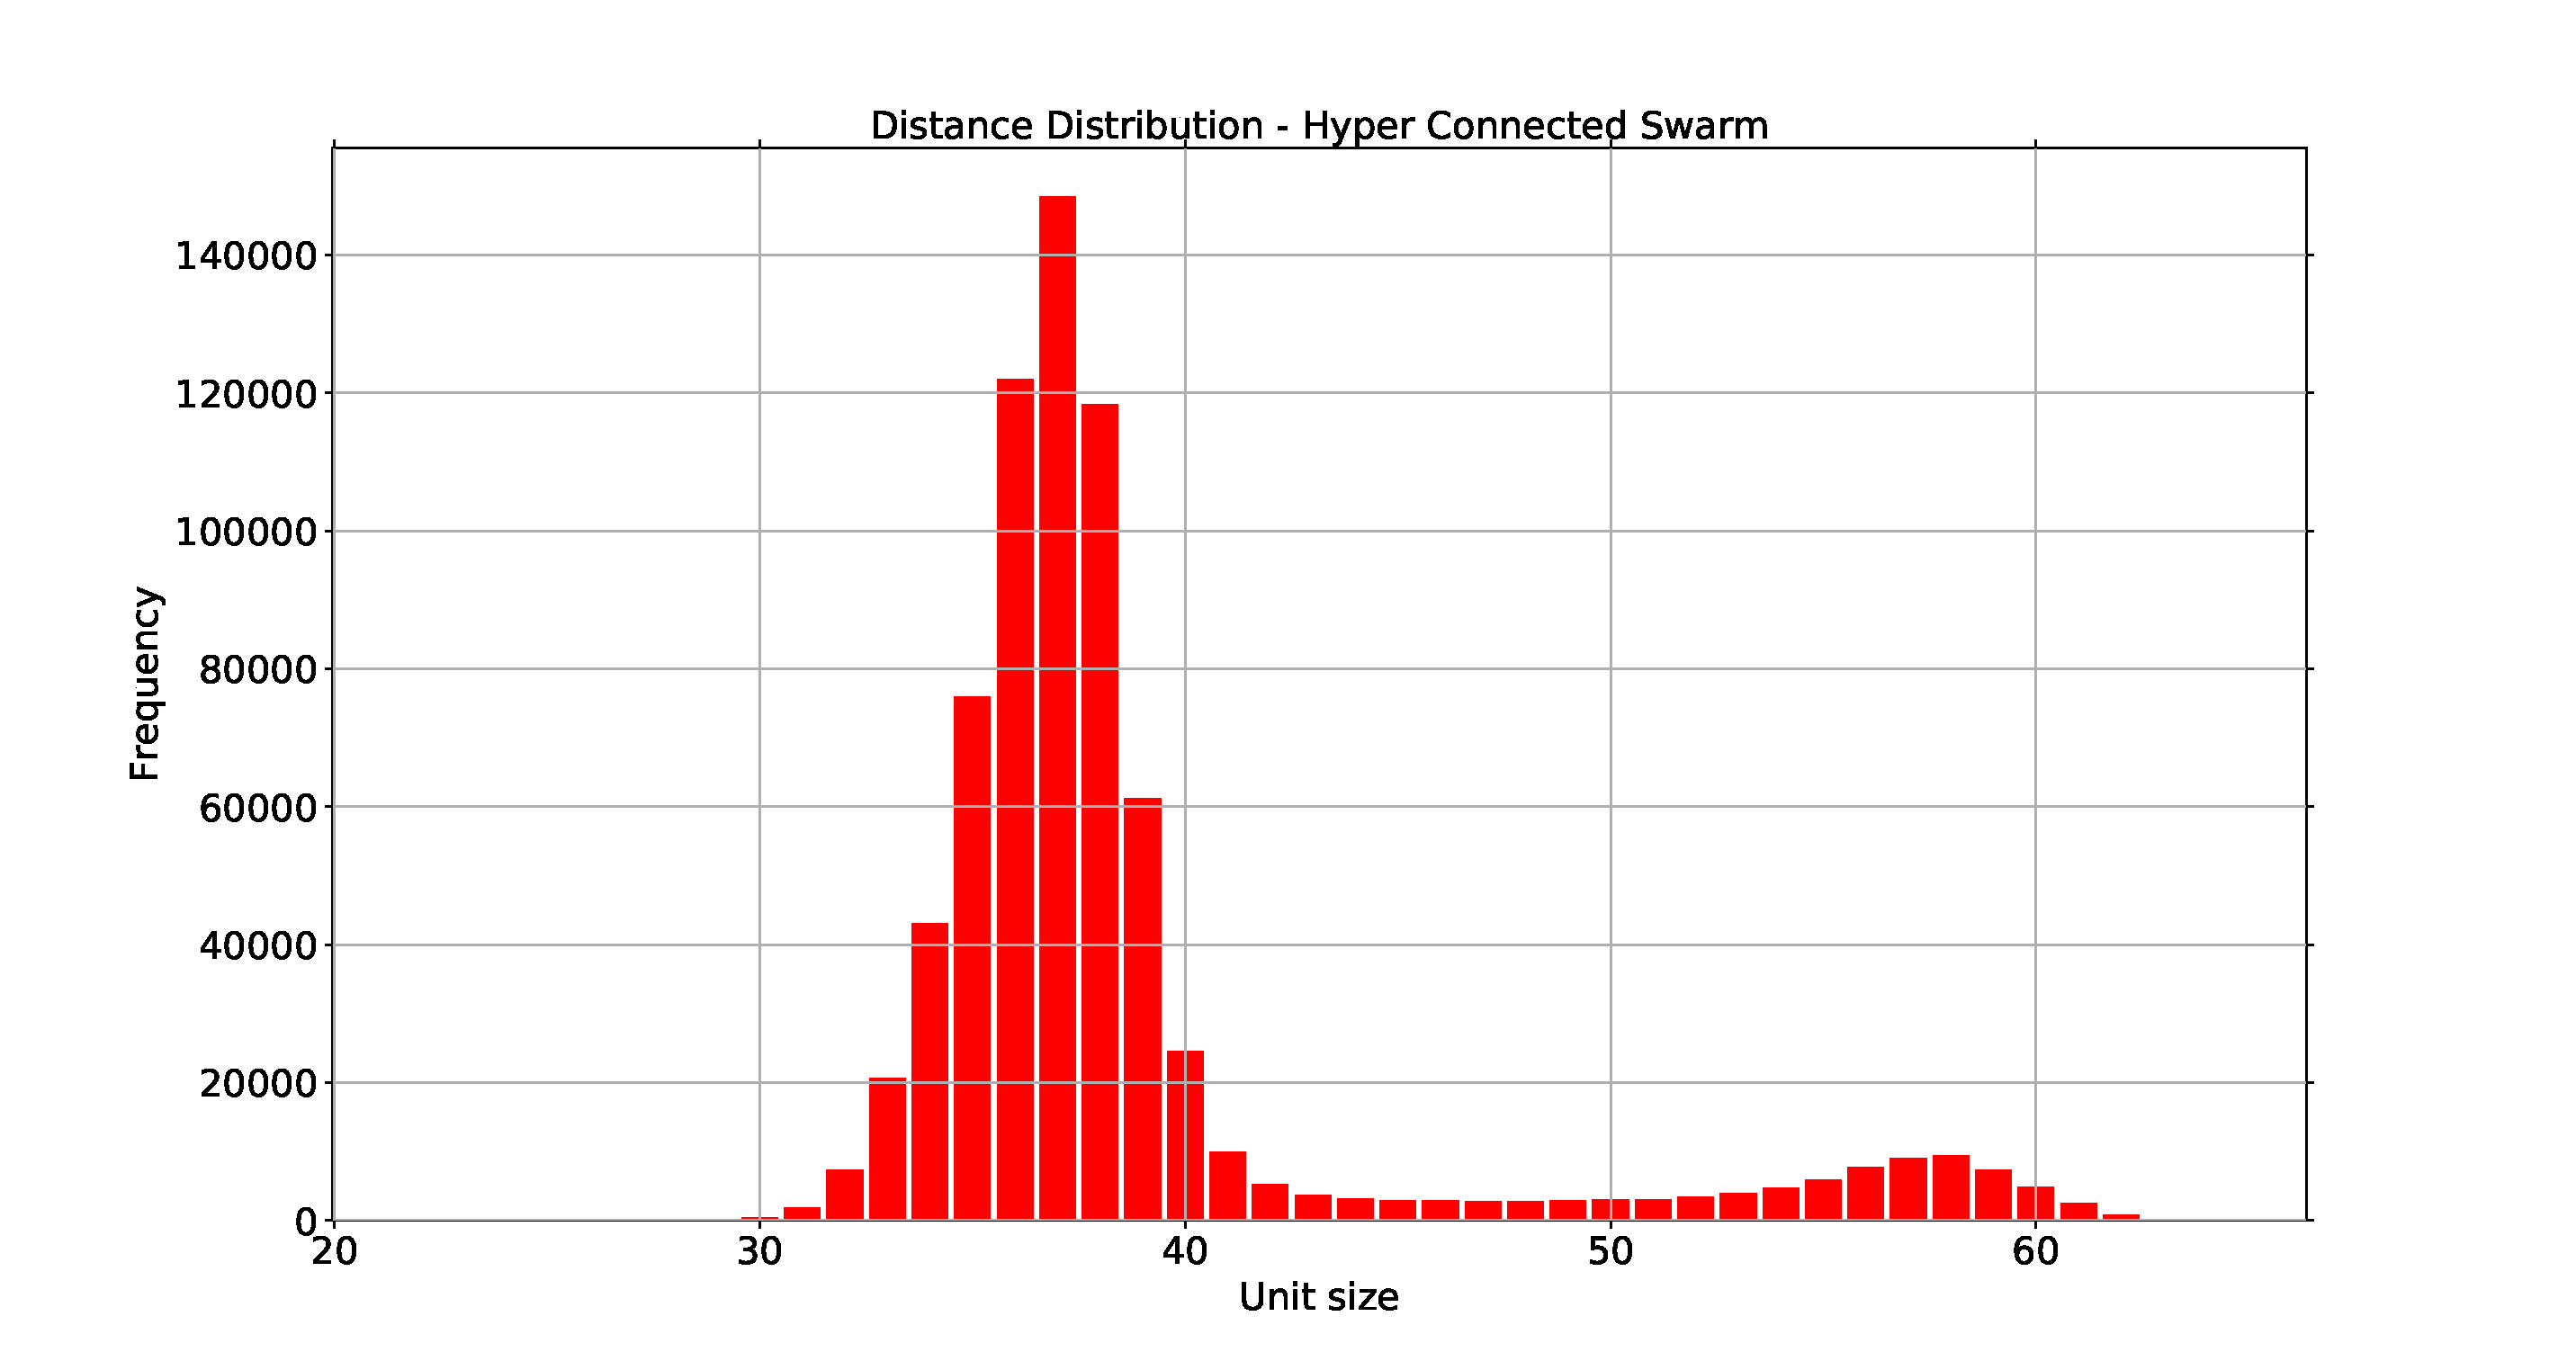
\includegraphics[width=13cm]{CHAPTER-5/figures/StabilityDistibutionHyper}
\end{center}
\caption{Distance distribution\label{methods:StabilityDistributionHyper}}
\end{figure}

\autoref{methods:StabilityDistributionHyper3D} shows the initial distribution of the agents and the progression of the distribution of the swarm agents until 10s into the simulation. The initial state of the distribution at 0s is the same for both swarm types. The impact of the field effects are immediate as the swarm stabilises to a bi-modal distribution. \autoref{methods:StabilityDistributionHyper3D2} shows the distribution of the data at 10 seconds (100 cycles) showing the resultant bi-modal frequencies the swarm is therefore a hyper-connected swarm.
%HYPER-DIST-BAR-3D.py
\begin{figure}[H]
\begin{center}
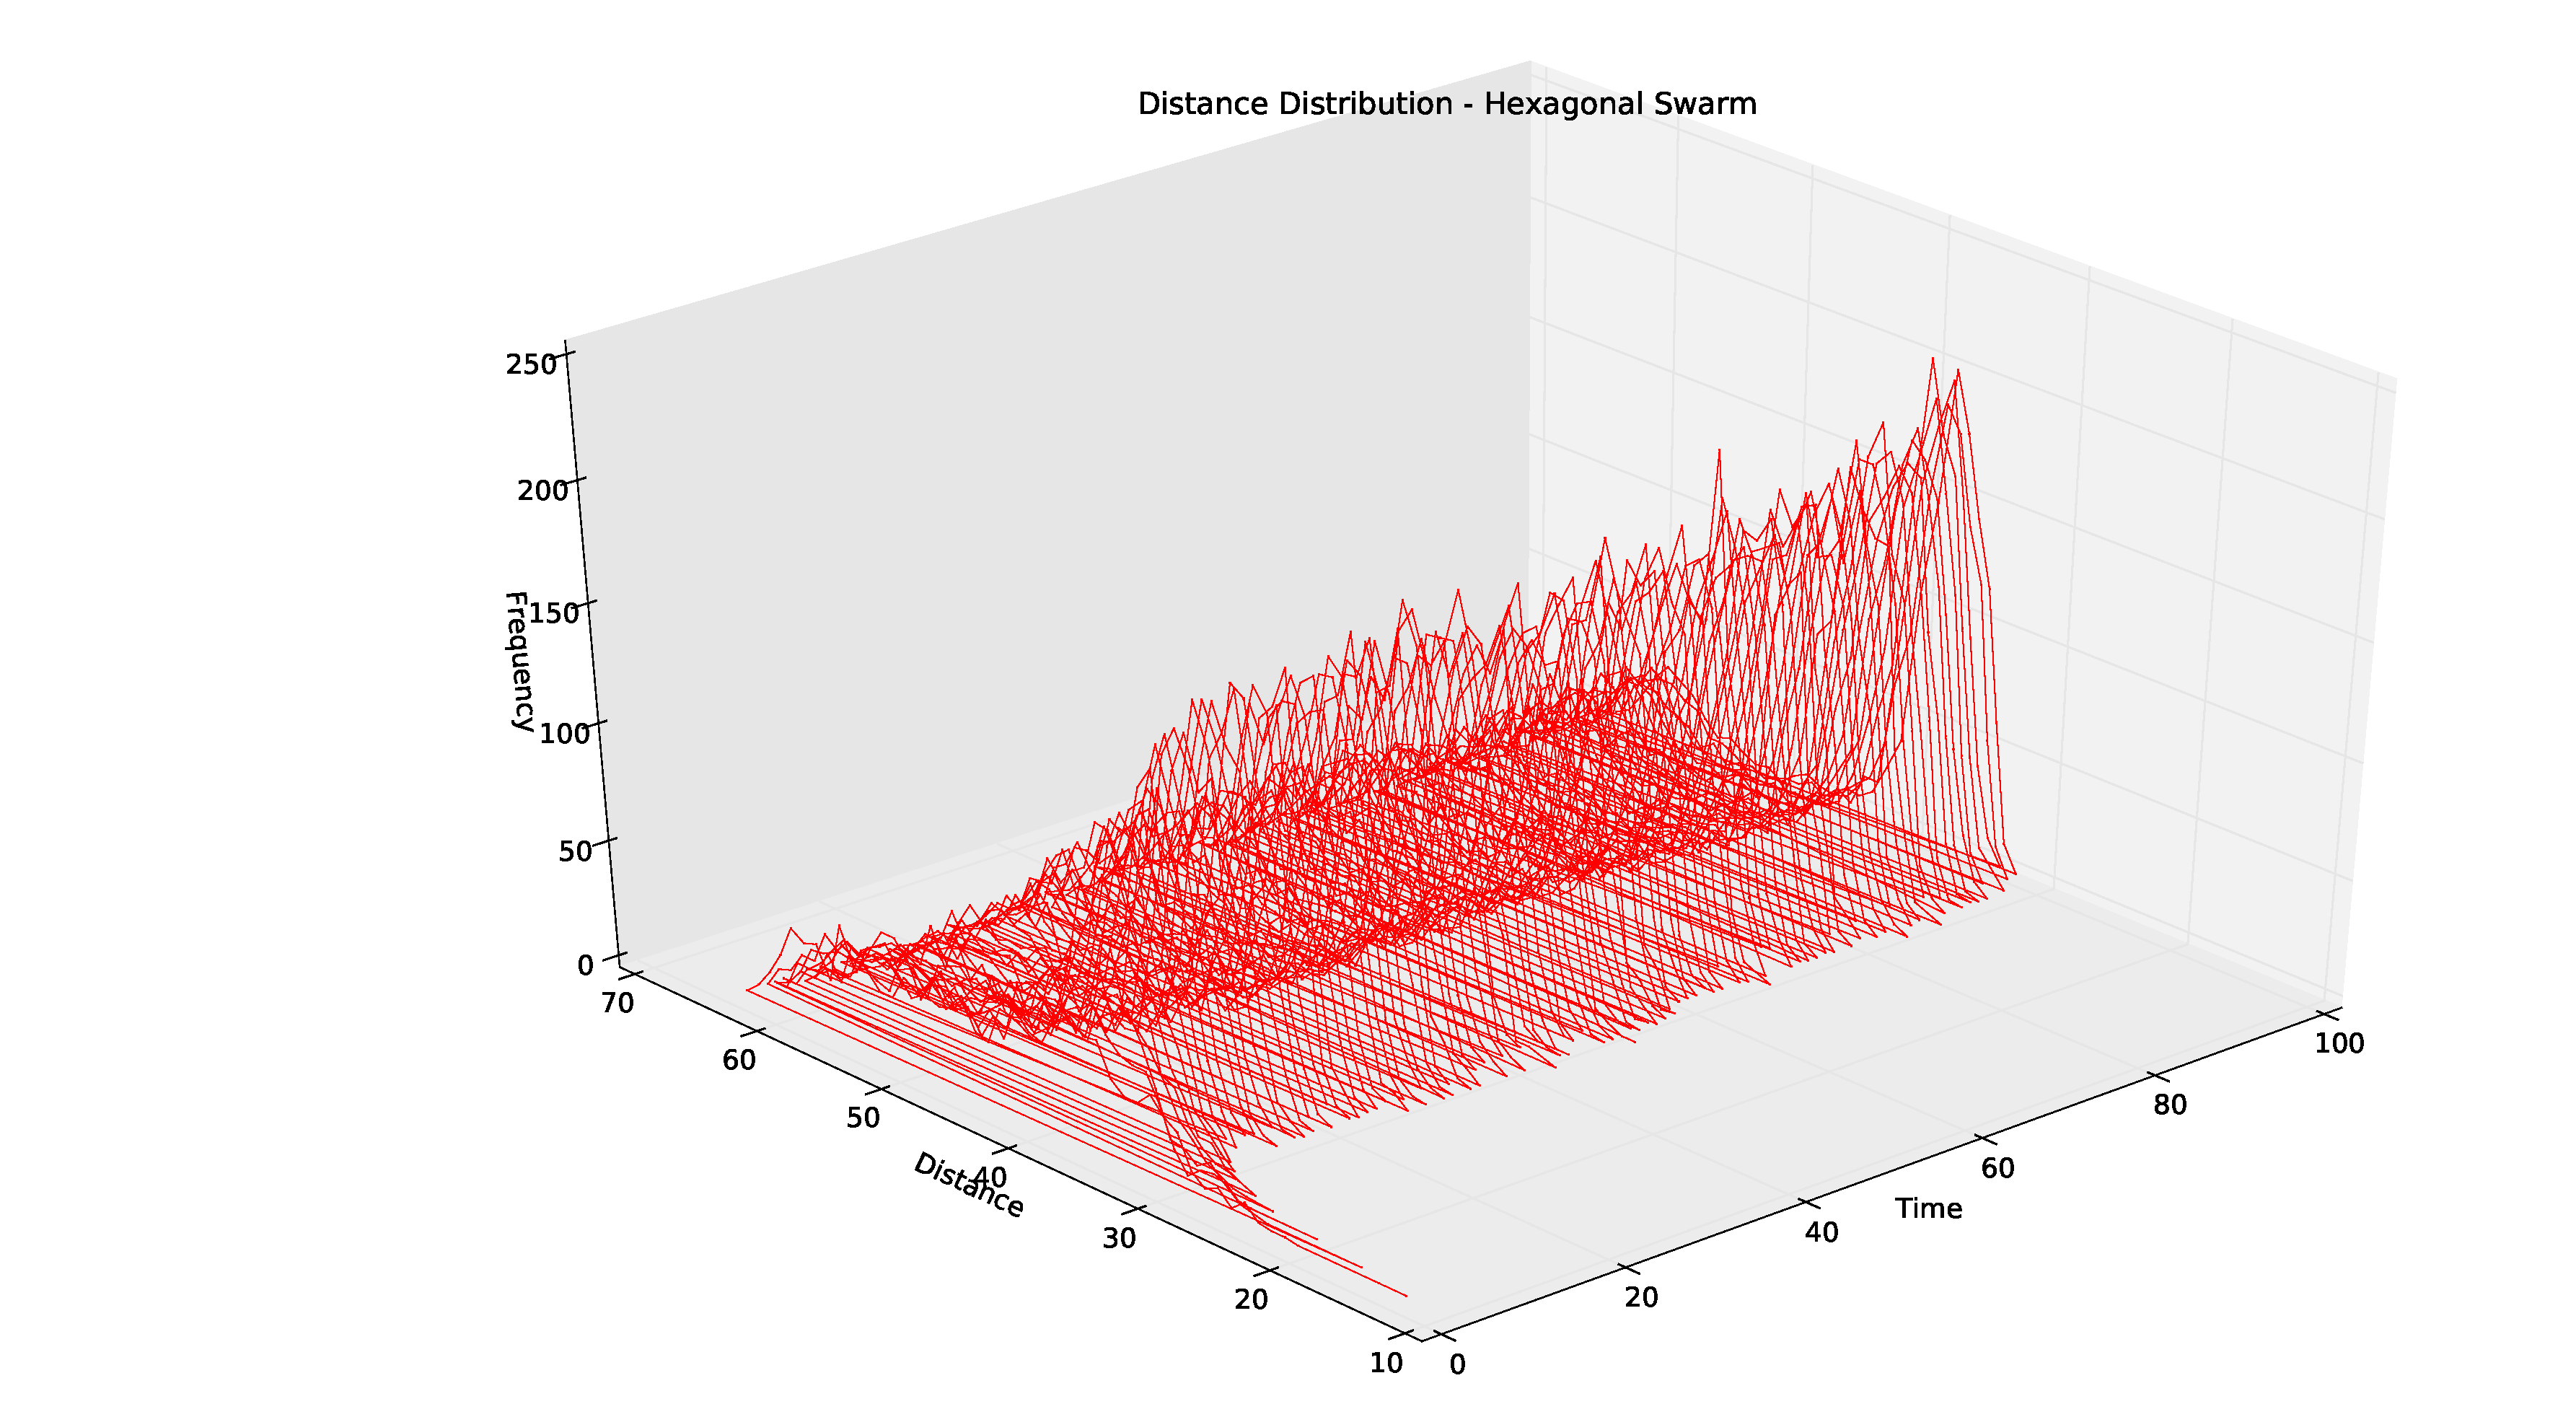
\includegraphics[width=13cm]{CHAPTER-5/figures/StabilityDistibutionHyper3D}
\end{center}
\caption{Distance distribution / Time 0-10 seconds\label{methods:StabilityDistributionHyper3D}}
\end{figure}

\begin{figure}[H]
\begin{center}
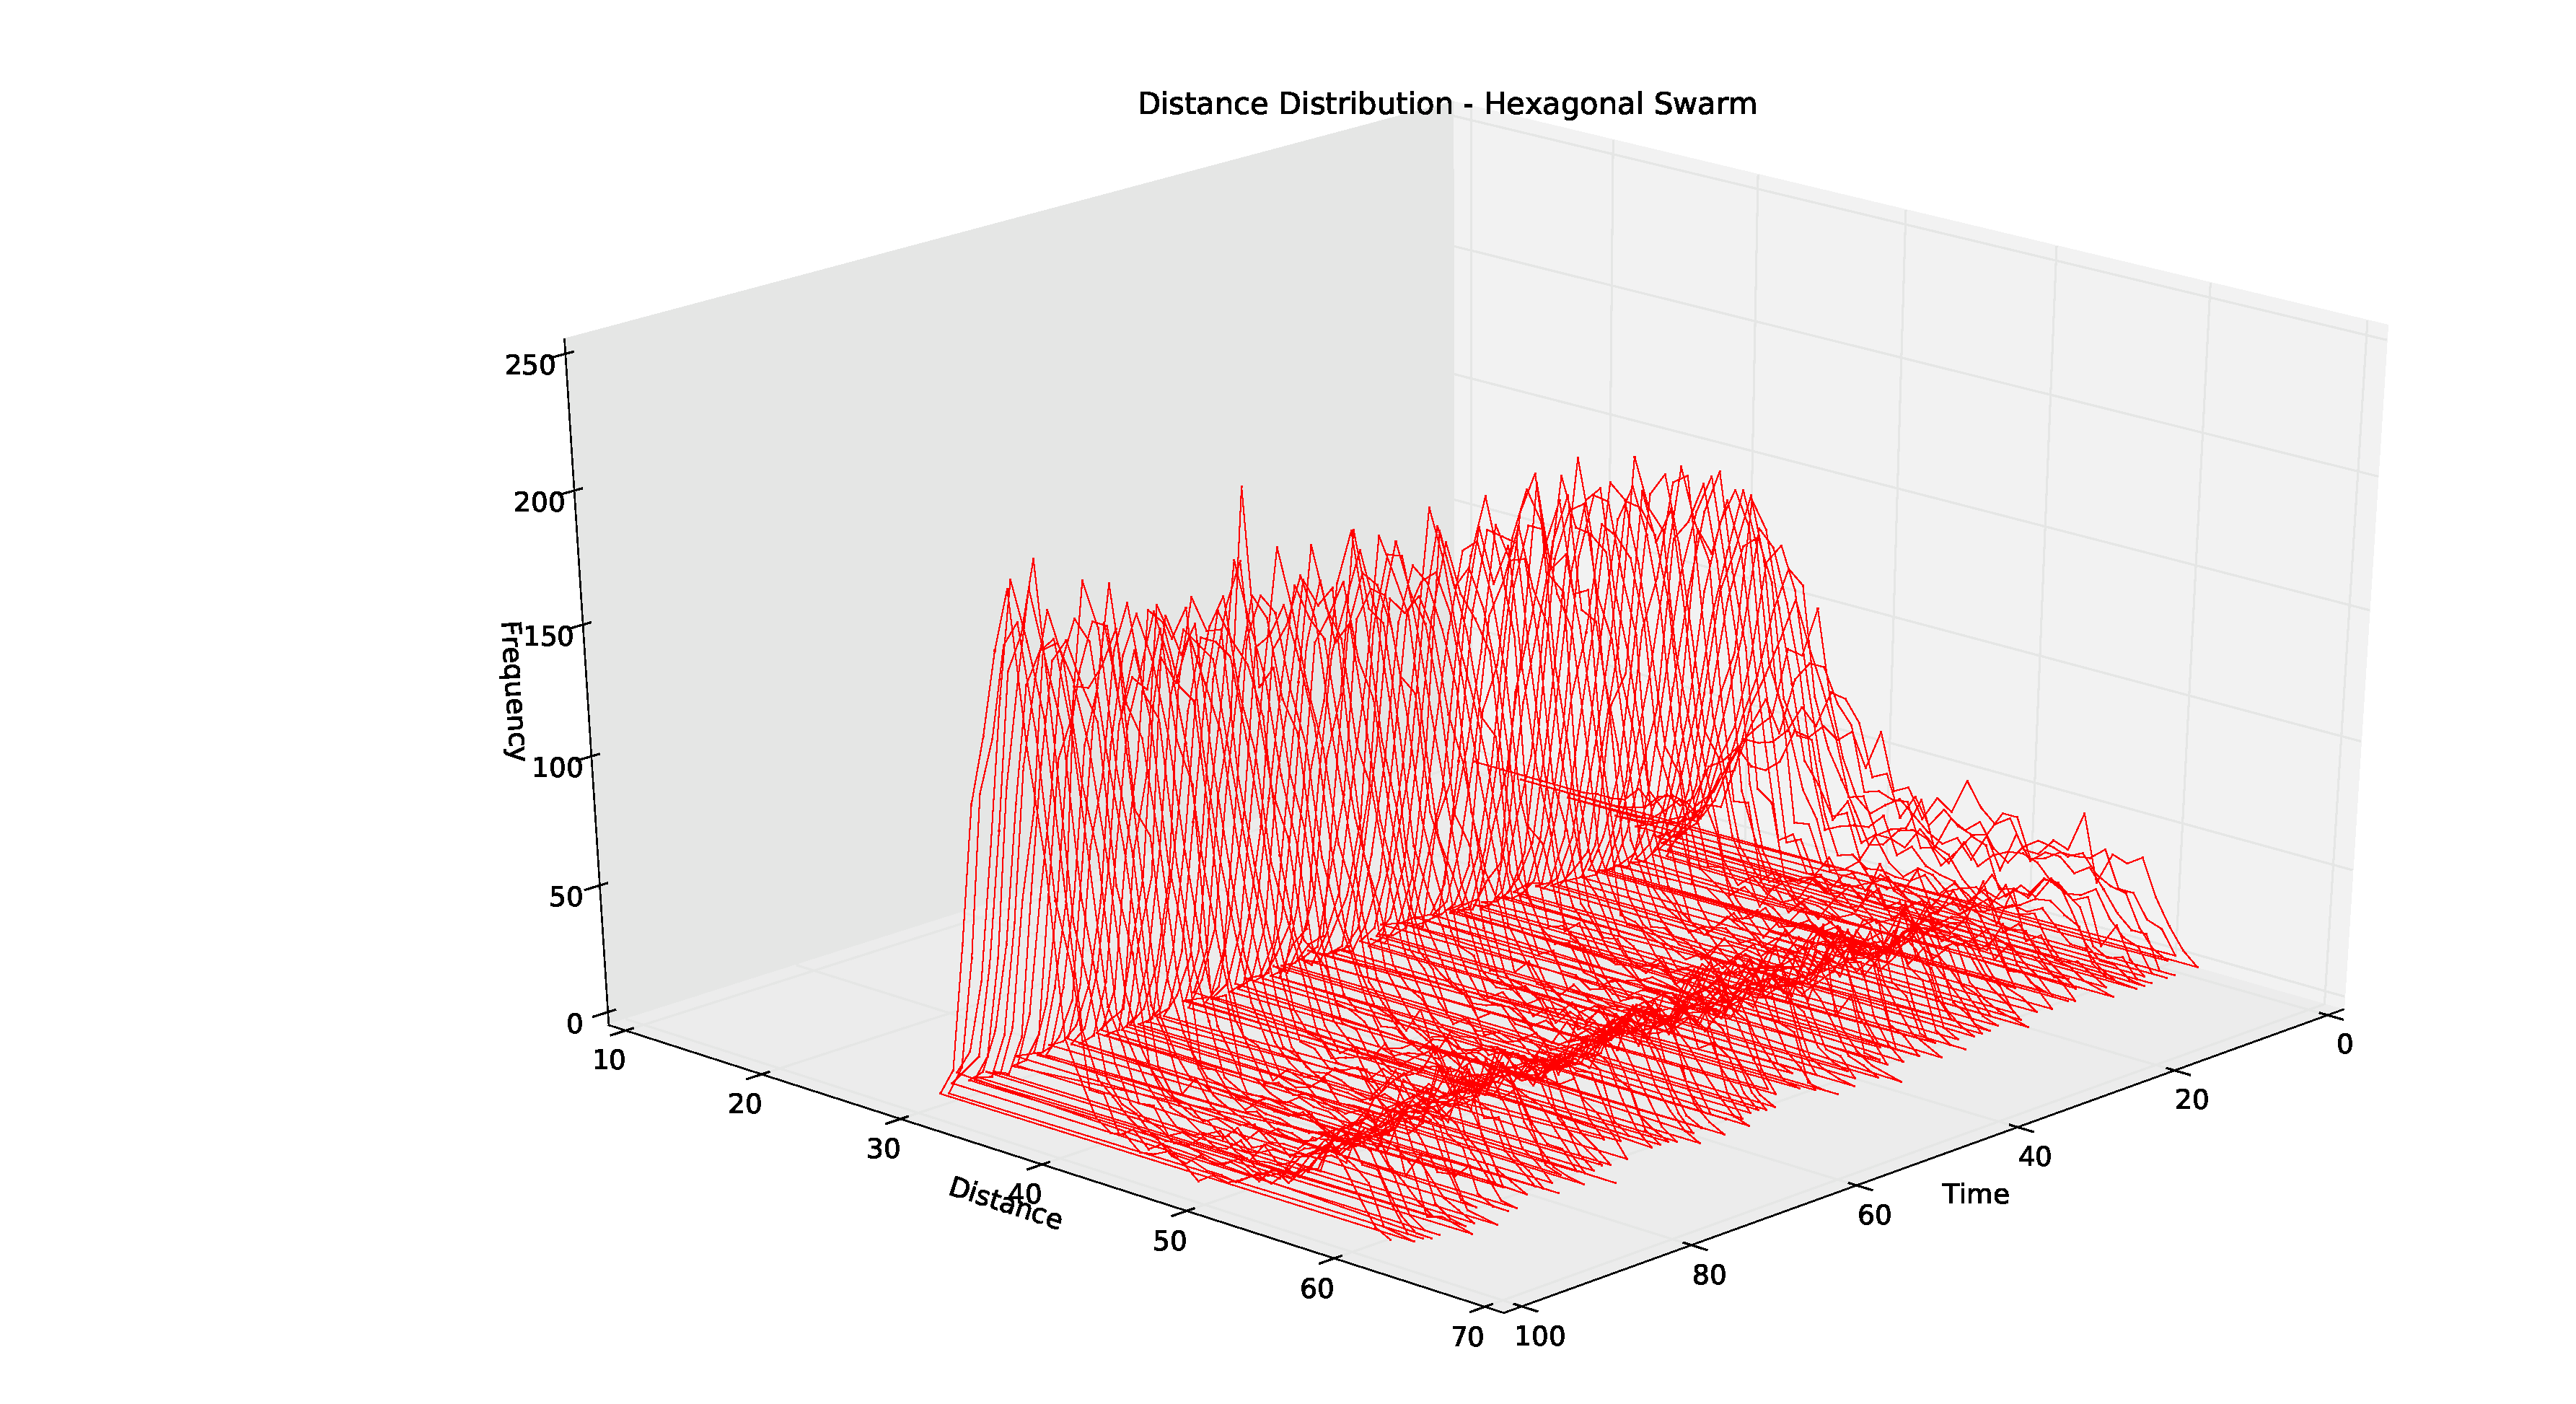
\includegraphics[width=13cm]{CHAPTER-5/figures/StabilityDistibutionHyper3D2}
\end{center}
\caption{Distance distribution / Time 10-0 seconds\label{methods:StabilityDistributionHyper3D2}}
\end{figure}

Although the field effects in this simulation have produced a bi-modal distribution increasing the neighbour distance will create further swarm types that will be multi-modal as more distant agents are identified as neighbours.

\subsection{Agent resultant magnitude based metric}
The distribution of the potential magnitudes can be visualised in the same way as the distances. \autoref{methods:StabilityMagnitudeHyper} shows the distribution of the agents based on potential magnitude for the entire duration of the simulation. As with the distance based metric the data forms a bi-modal distribution with a mean magnitude as shown in \autoref{methods:StabilityMagnitude40-60}. \autoref{methods:StabilityMagnitudeHyper} shows negative magnitudes which indicates sections of the swarm are expanding. 
%HYPER-MAG.py
\begin{figure}[H]
\begin{center}
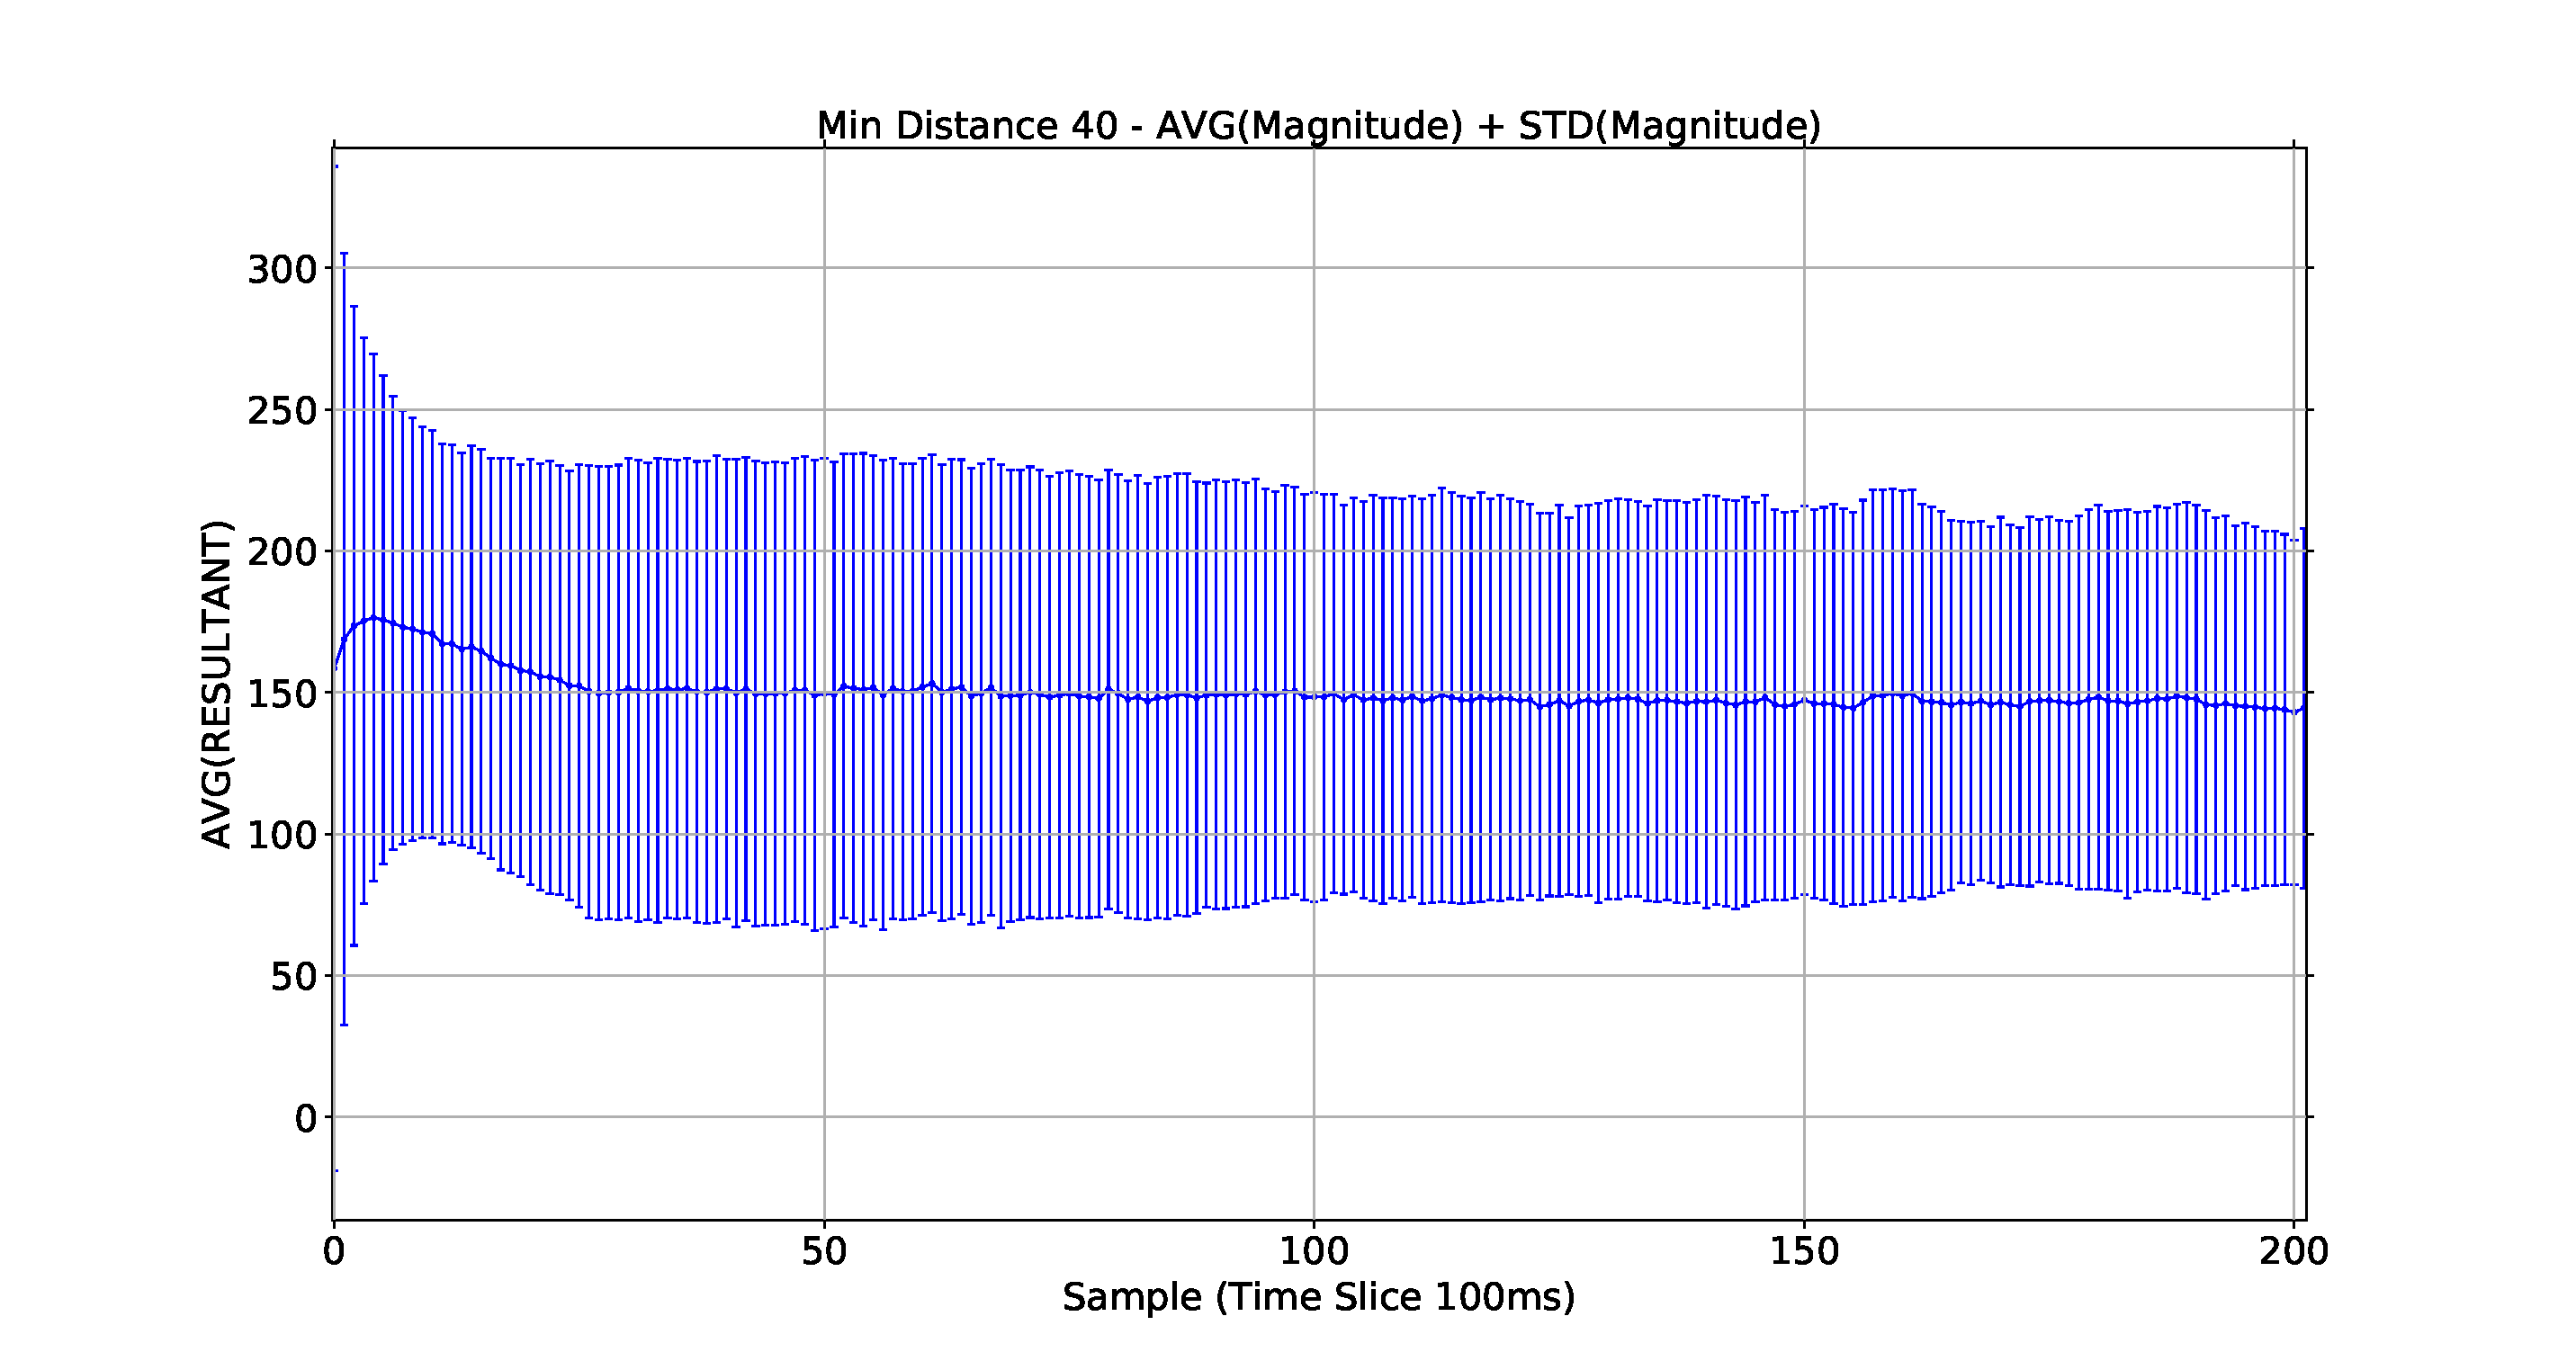
\includegraphics[width=13cm]{CHAPTER-5/figures/StabilityMagnitudeSwarm40-60}
\end{center}
\caption{Agent resultant magnitude metric\label{methods:StabilityMagnitude40-60}}
\end{figure}
%HYPER-MAG-BAR.py 
\begin{figure}[H]
\begin{center}
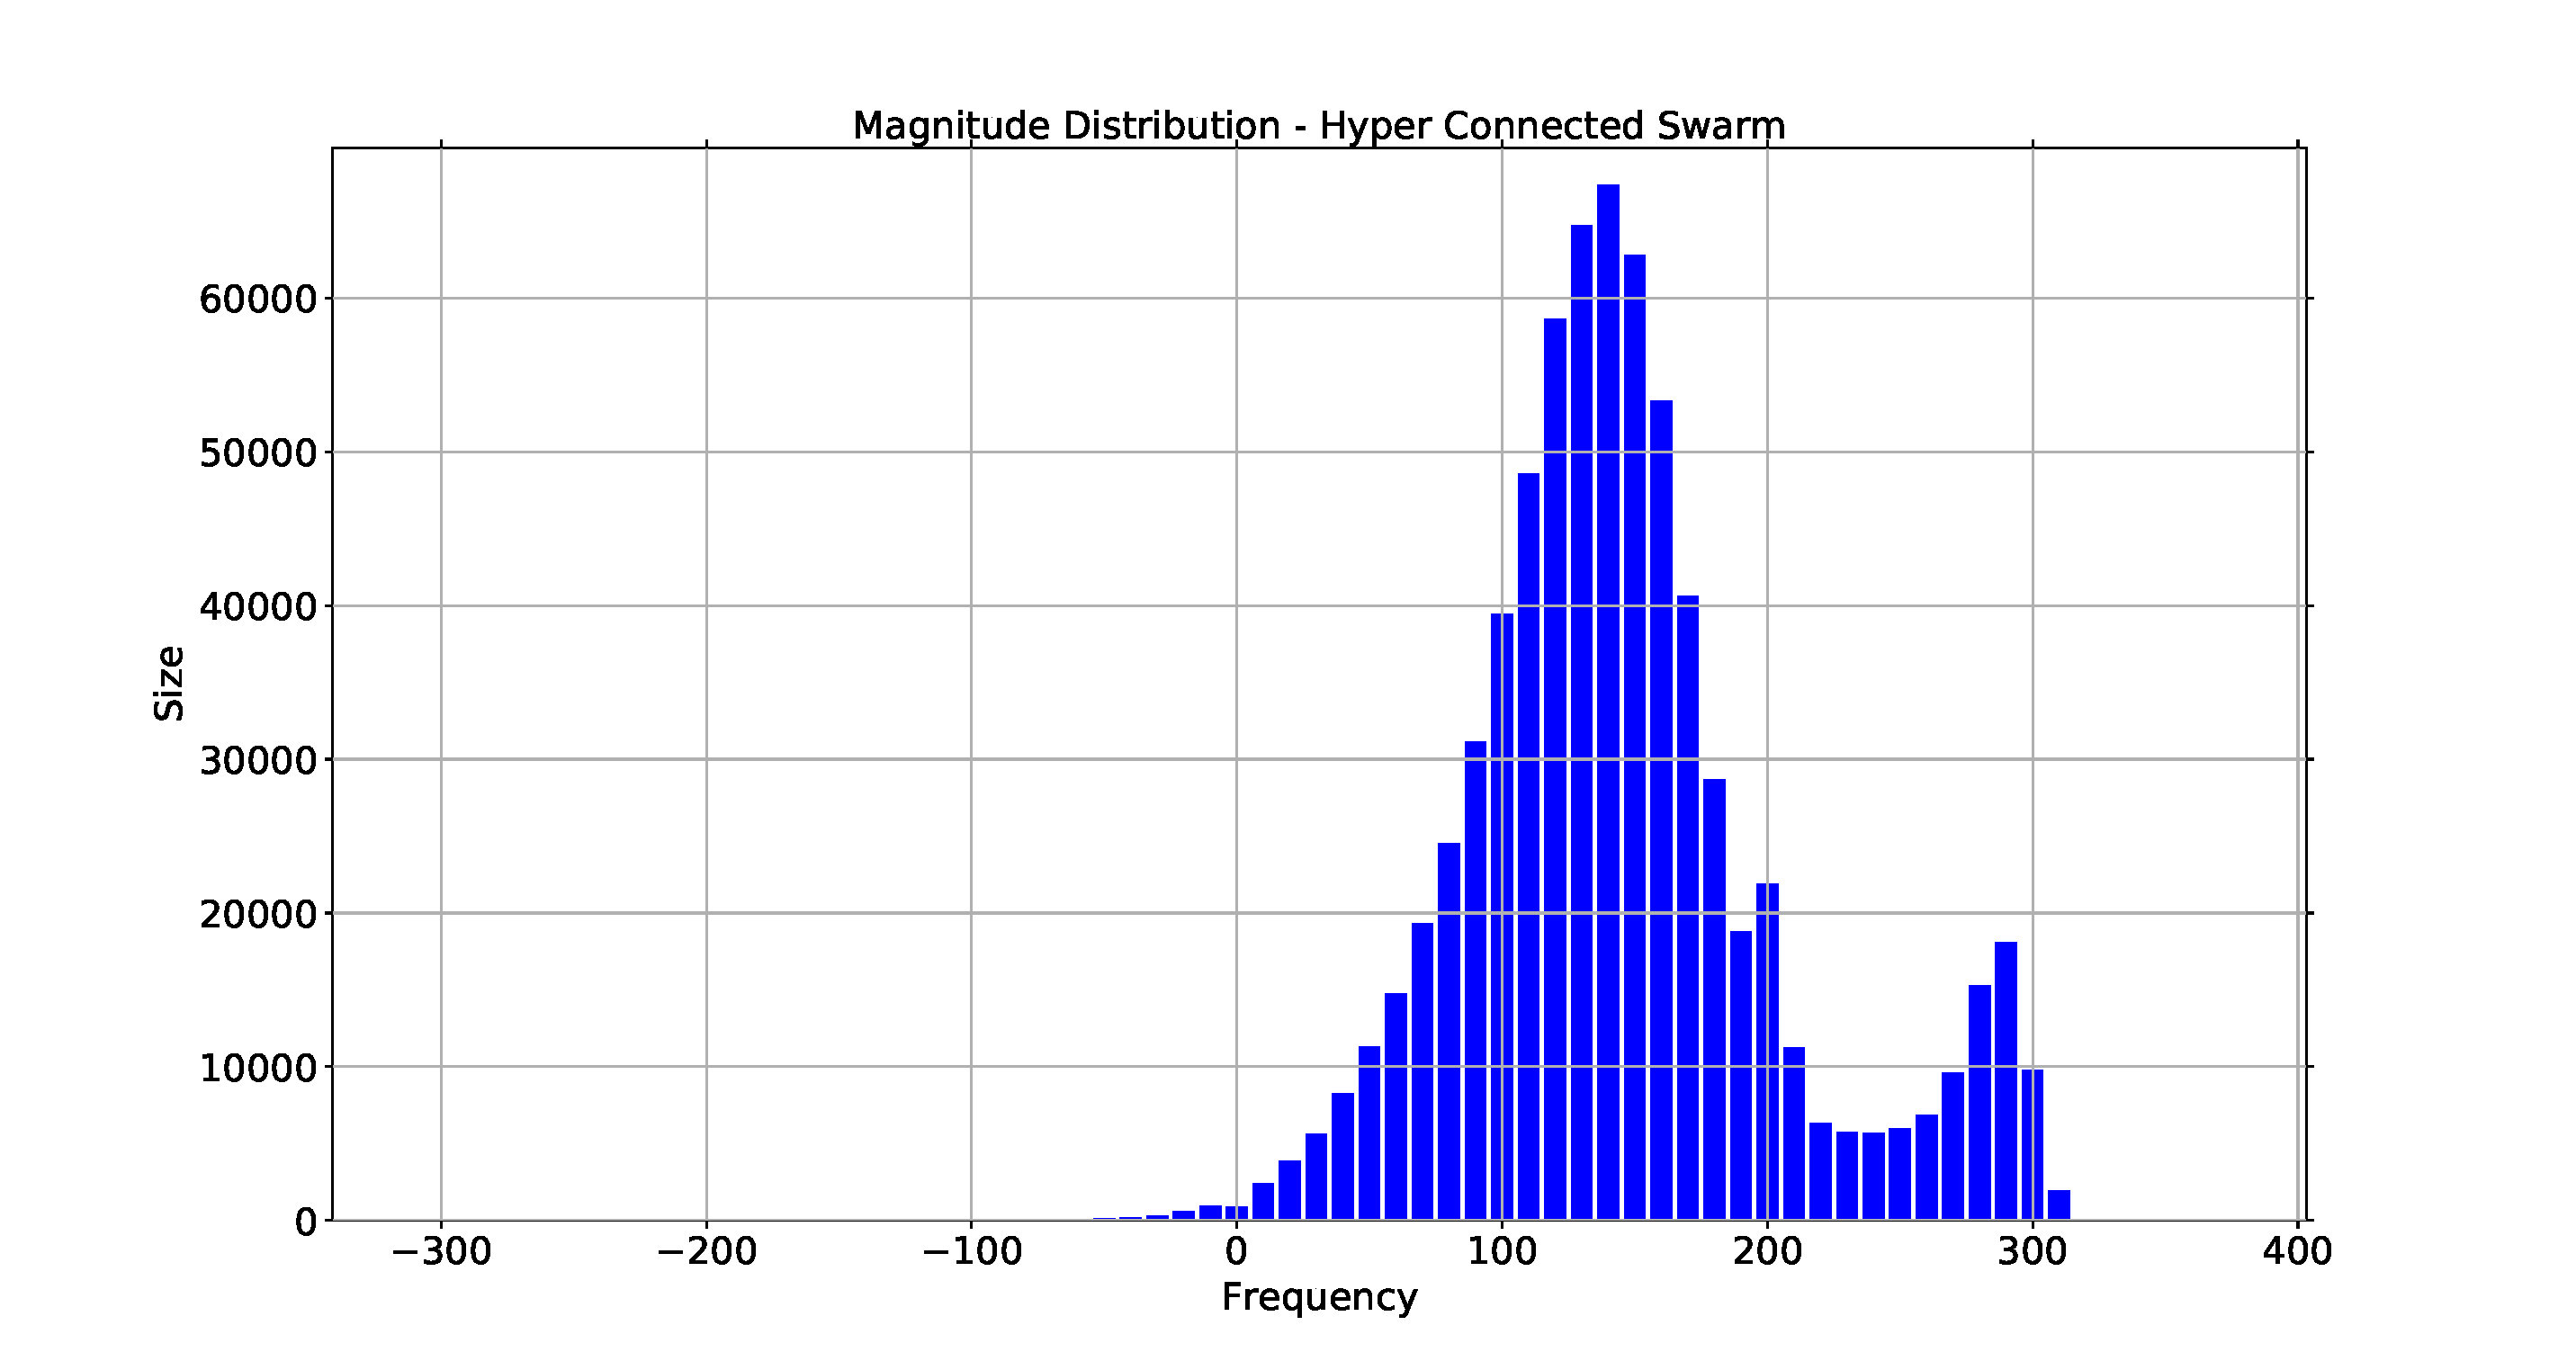
\includegraphics[width=13cm]{CHAPTER-5/figures/StabilityMagnitudeHyper}
\end{center}
\caption{Agent resultant magnitude distribution\label{methods:StabilityMagnitudeHyper}}
\end{figure}

\autoref{methods:StabilityMagHyper3D} and \ref{methods:StabilityMagHyper3D2} show the distributions at each time cycle and visualise the change in the distributions of the agent resultant magnitudes. As with the distance visualisations \autoref{methods:StabilityMagHyper3D} shows the initial distribution at time interval 0 to 100 and \autoref{methods:StabilityMagHyper3D2} shows the final state of the swarm after 10 seconds (100 cycles). Both show the bi-model state of the swarm emerging.
%HYPER-MAG-BAR-3D.py
\begin{figure}[H]
\begin{center}
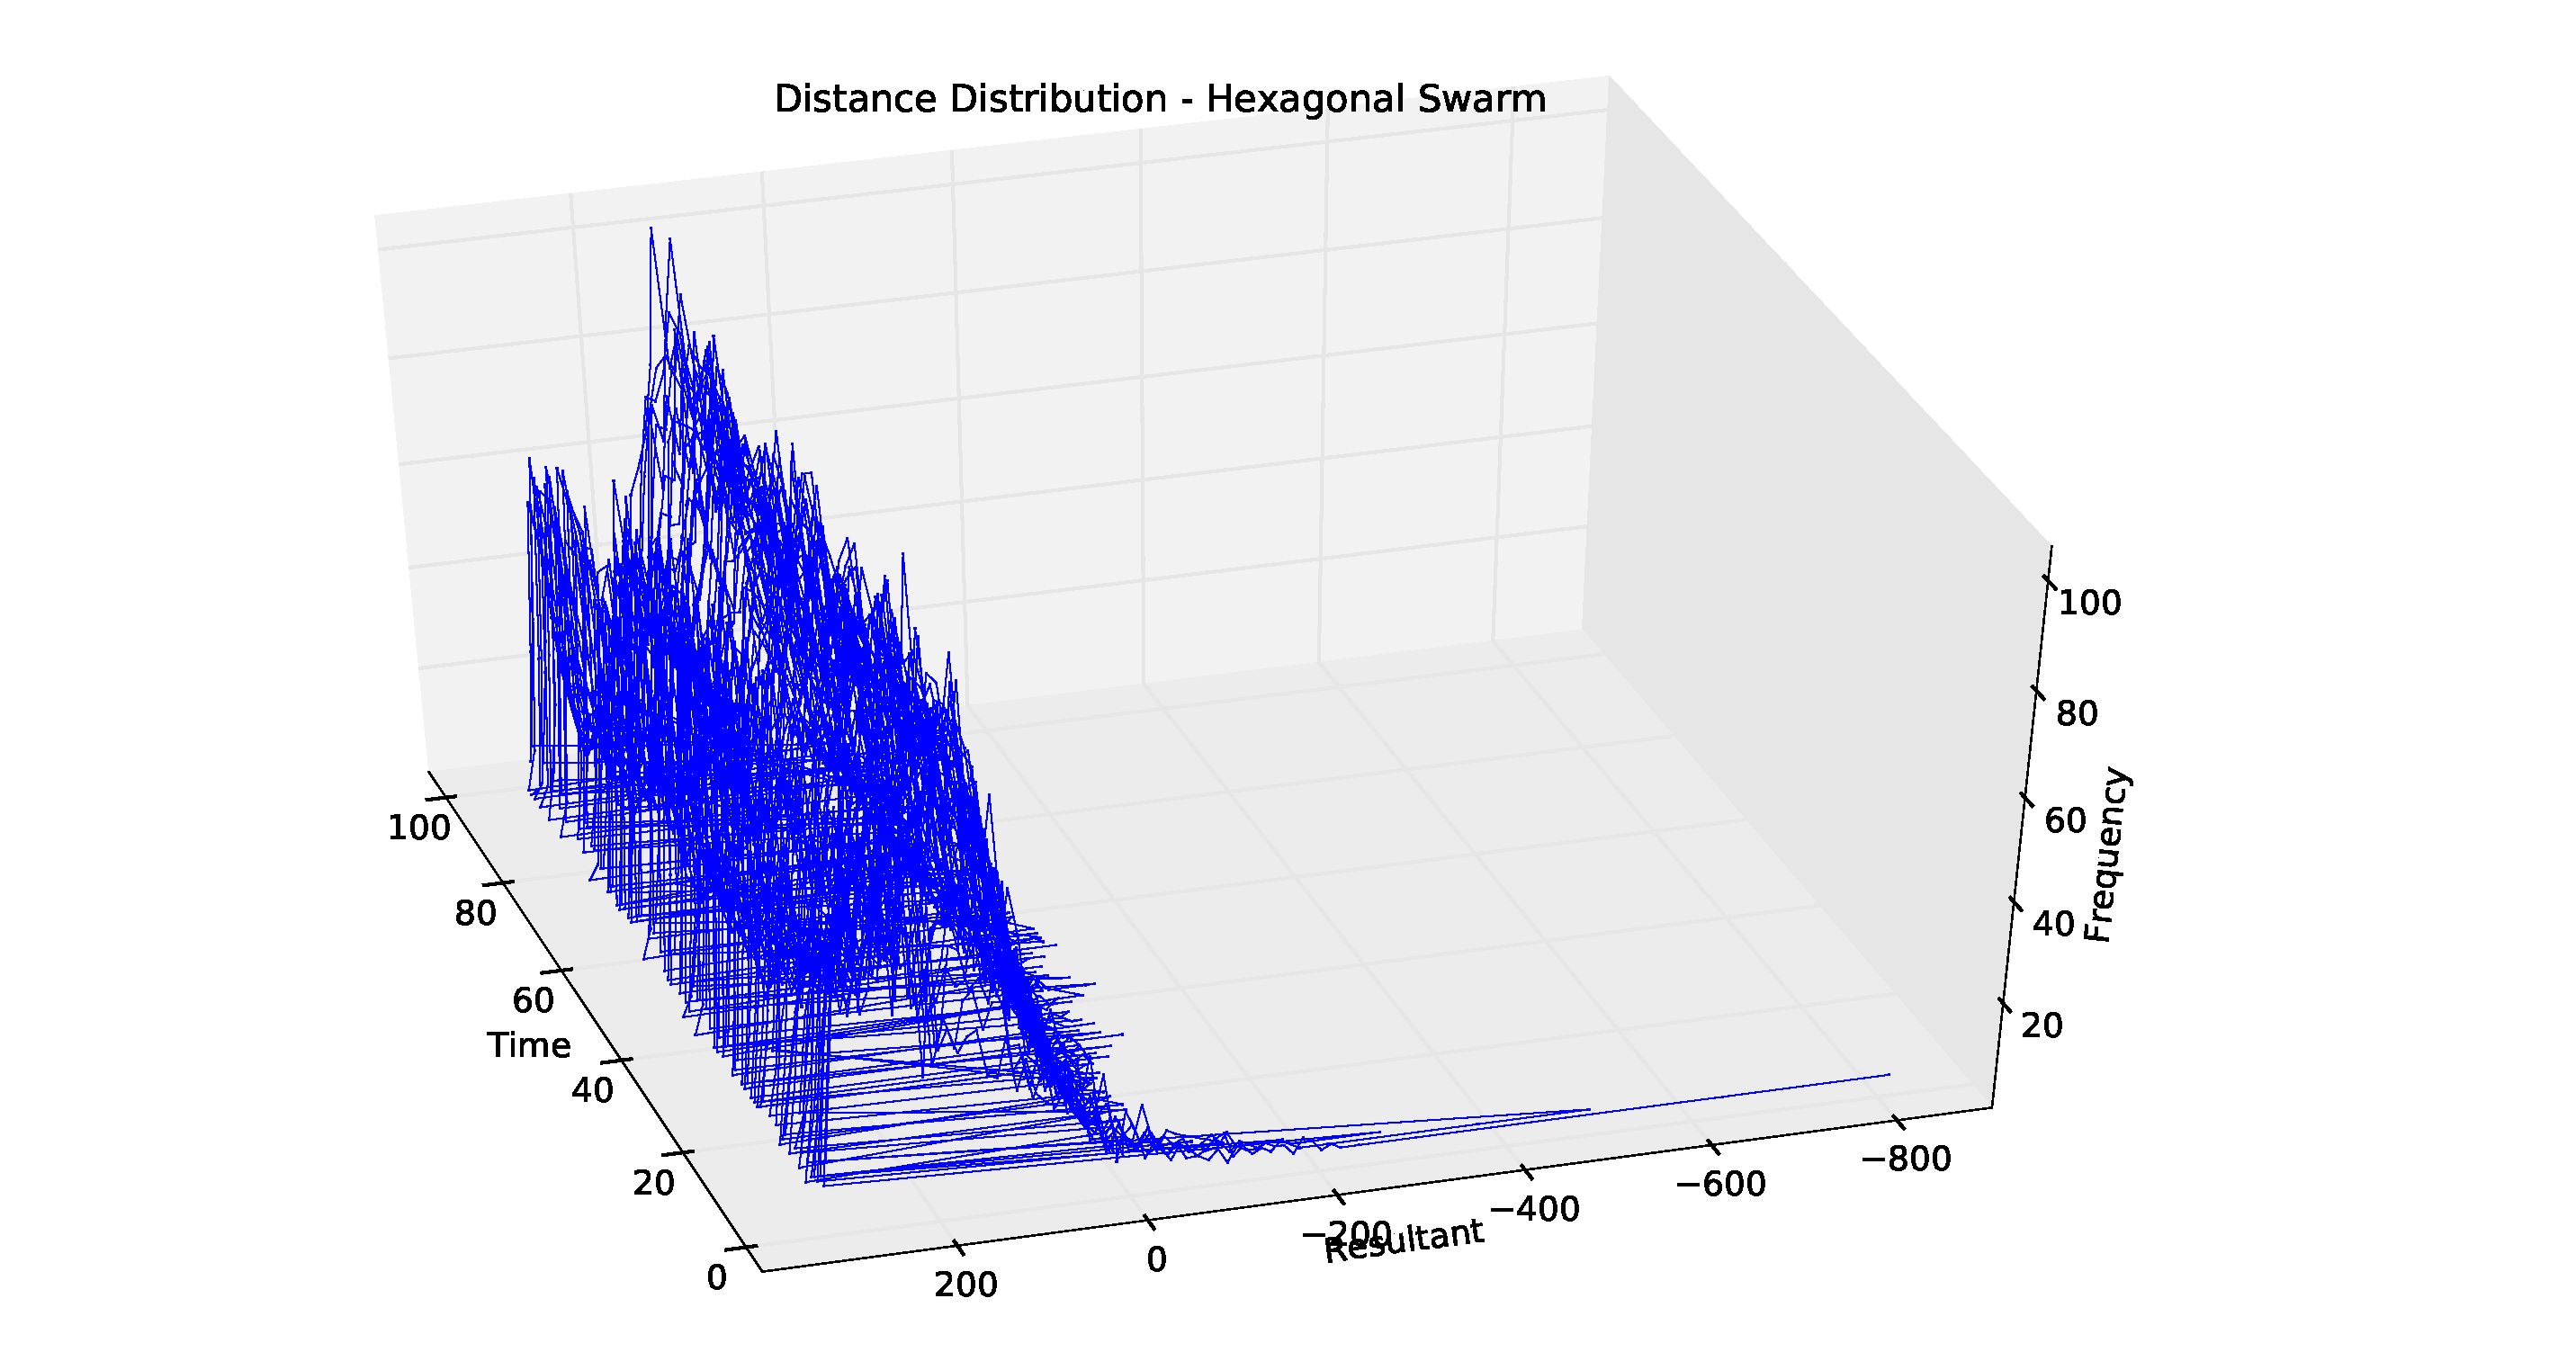
\includegraphics[width=13cm]{CHAPTER-5/figures/StabilityMagHyper3D}
\end{center}
\caption{Agent resultant magnitude distribution / Time 0-10s\label{methods:StabilityMagHyper3D}}
\end{figure}

\begin{figure}[H]
\begin{center}
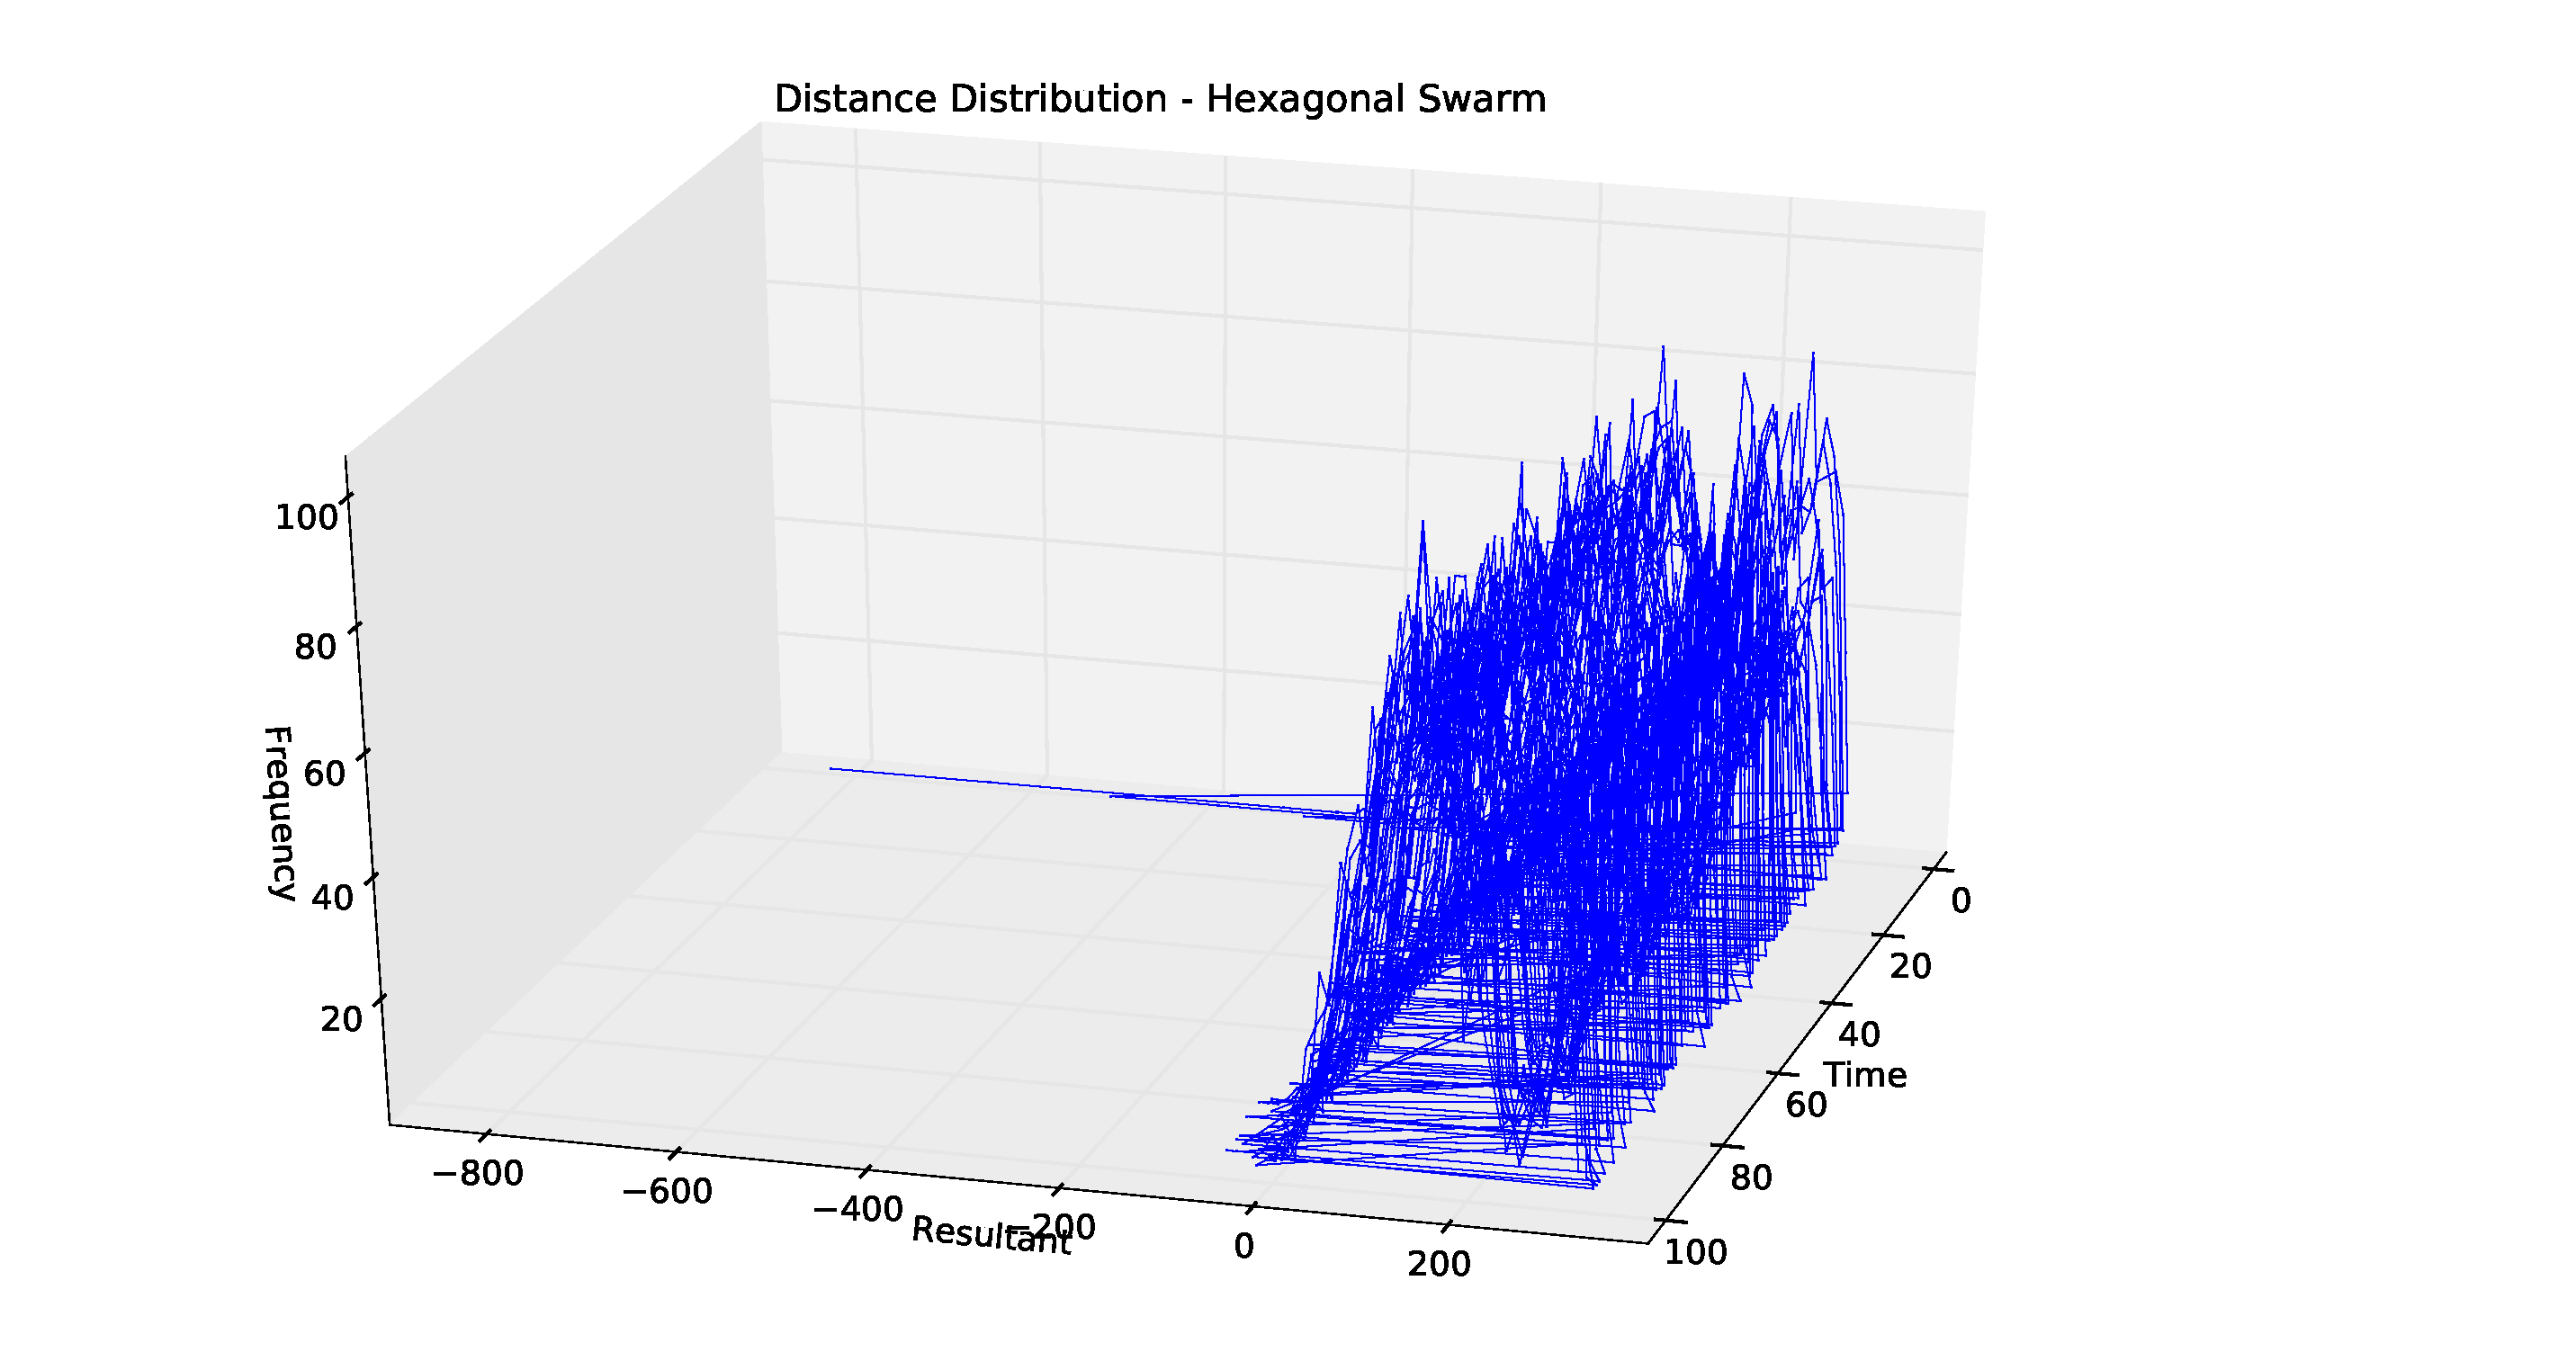
\includegraphics[width=13cm]{CHAPTER-5/figures/StabilityMagHyper3D2}
\end{center}
\caption{Agent resultant magnitude distribution / Time 10-0s\label{methods:StabilityMagHyper3D2}}
\end{figure}

\section{Metric comparison\label{section:stabilityComparison}}
Looking at the two swarm types together the characteristics of the swarm types present themselves as change in the standard deviation from either the average distance or the average magnitude of the agents in the swarm.

\autoref{methods:StabilityDistanceSwarm40-5060} shows the swarm with the two different field effects for cohesion. The metric used in this analysis is the distance between agents. The result shows that the deviation on the hyper-connected swarm (shown in green) has a higher standard deviation than the hexagonal swarm (shown in brown). This is caused by the bi-modal nature of the hyper-connected swarm.

\autoref{methods:StabilityMagnitudeSwarm40-5060} shows the analysis of the agent resultant magnitude between the agents in the swarm which demonstrates the same characteristic emerging.
%HEX-HYPER.py
\begin{figure}[H]
\begin{center}
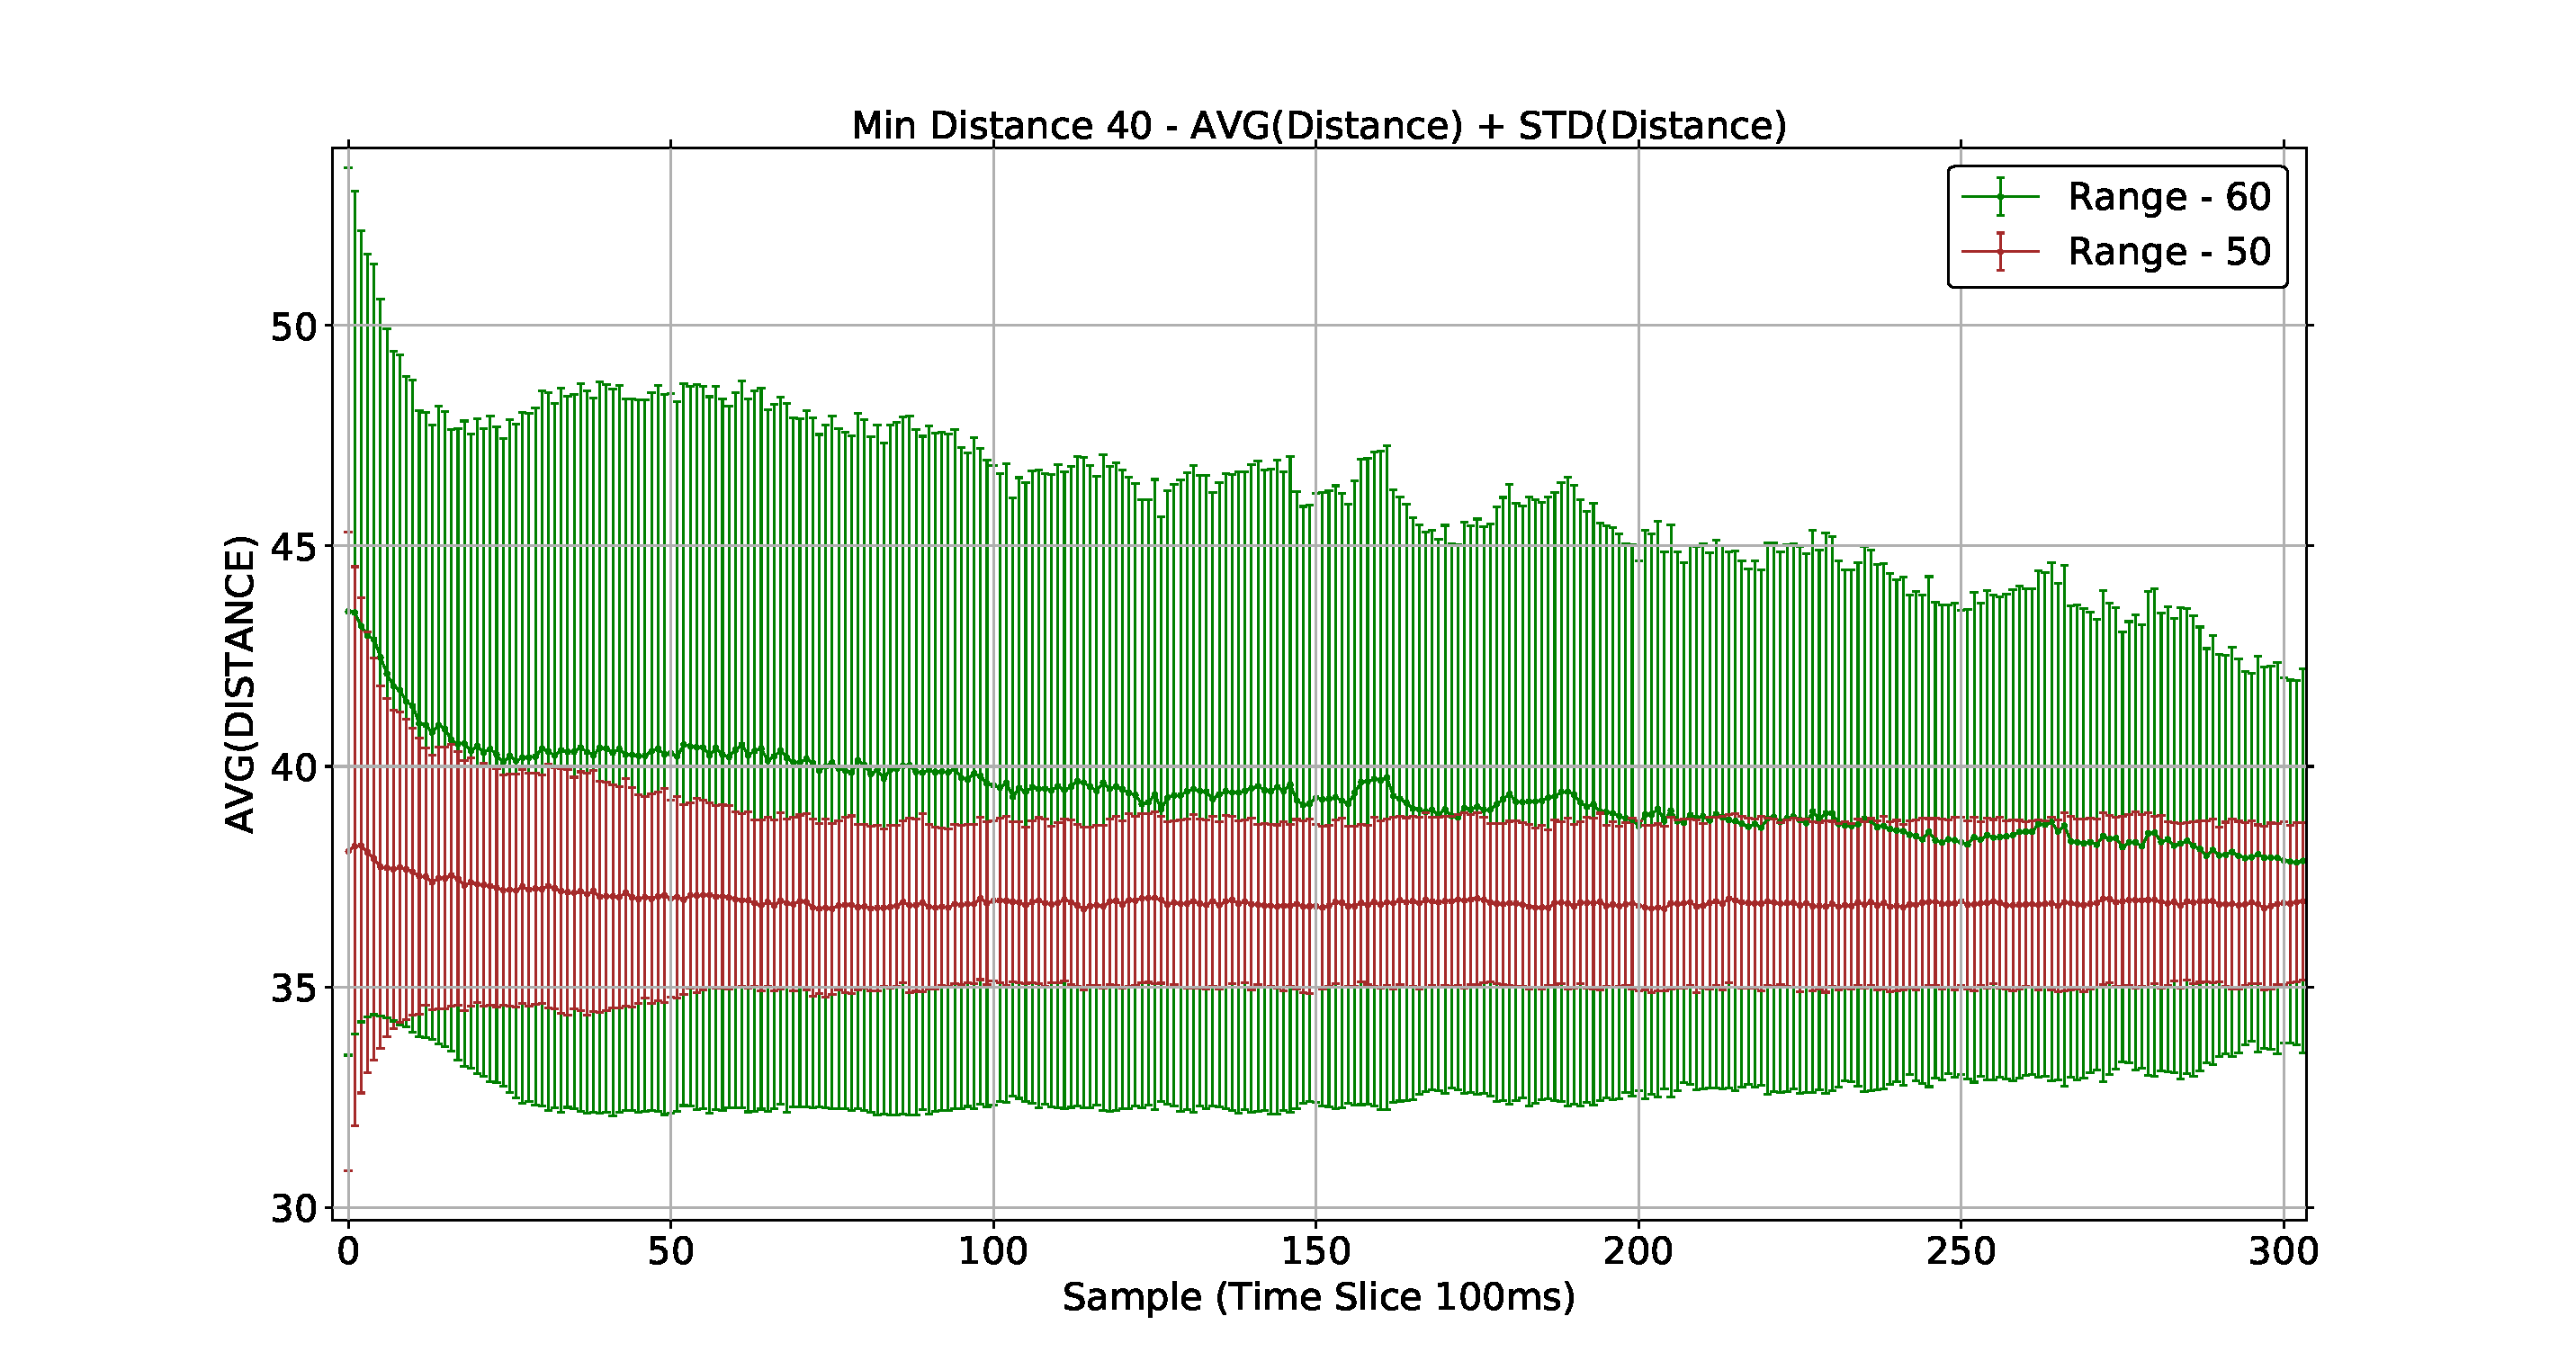
\includegraphics[width=13cm]{CHAPTER-5/figures/StabilityDistanceSwarm40-5060}
\end{center}
\caption{Distances metric comparison\label{methods:StabilityDistanceSwarm40-5060}}
\end{figure}
%HEX-HYPER-MAG.py
\begin{figure}[H]
\begin{center}
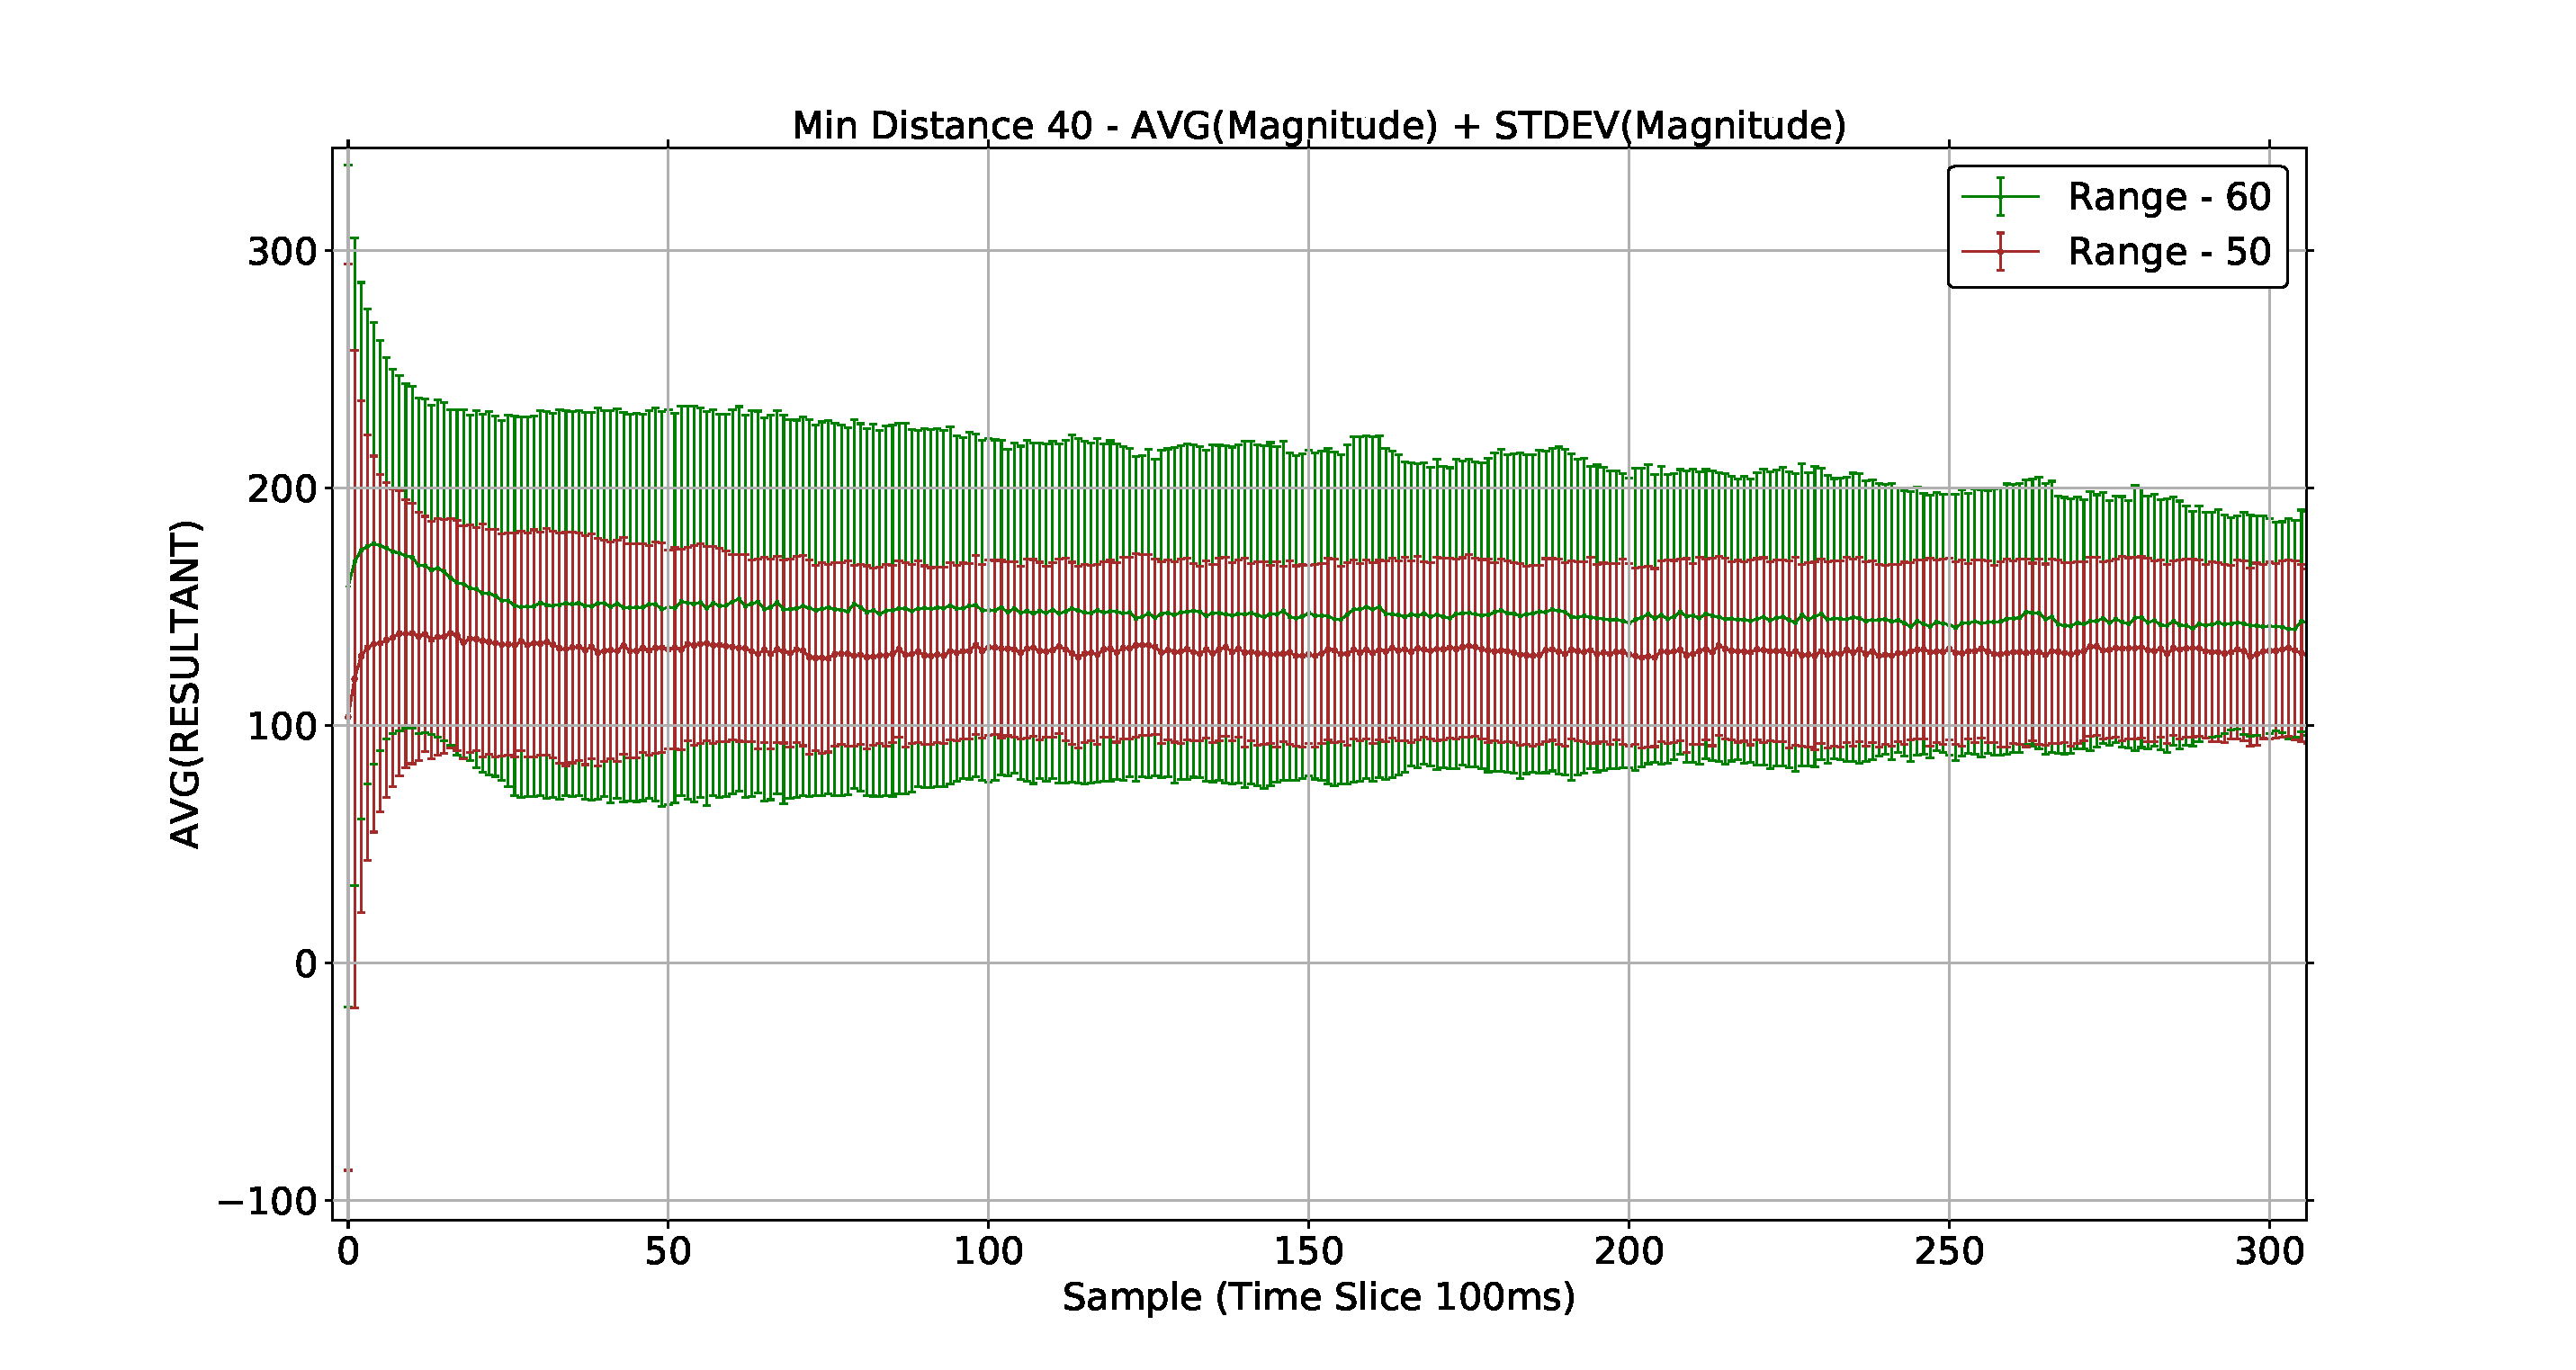
\includegraphics[width=13cm]{CHAPTER-5/figures/StabilityMagnitudeSwarm40-5060}
\end{center}
\caption{Agent resultant magnitude metric comparison\label{methods:StabilityMagnitudeSwarm40-5060}}
\end{figure}

A well structured and balanced swarm should therefore have a very low standard deviation in terms of the resultant metric. Figures~\ref{methods:StabilityDistanceSwarm} and~\ref{methods:StabilityMagnitudeSwarm} clearly show using either magnitude or distance as the metric that the deviation from the mean can highlight the two different types of swarm when using the same repulsion field setting.
%HEX-HYPER-STD.py
\begin{figure}[H]
\begin{center}
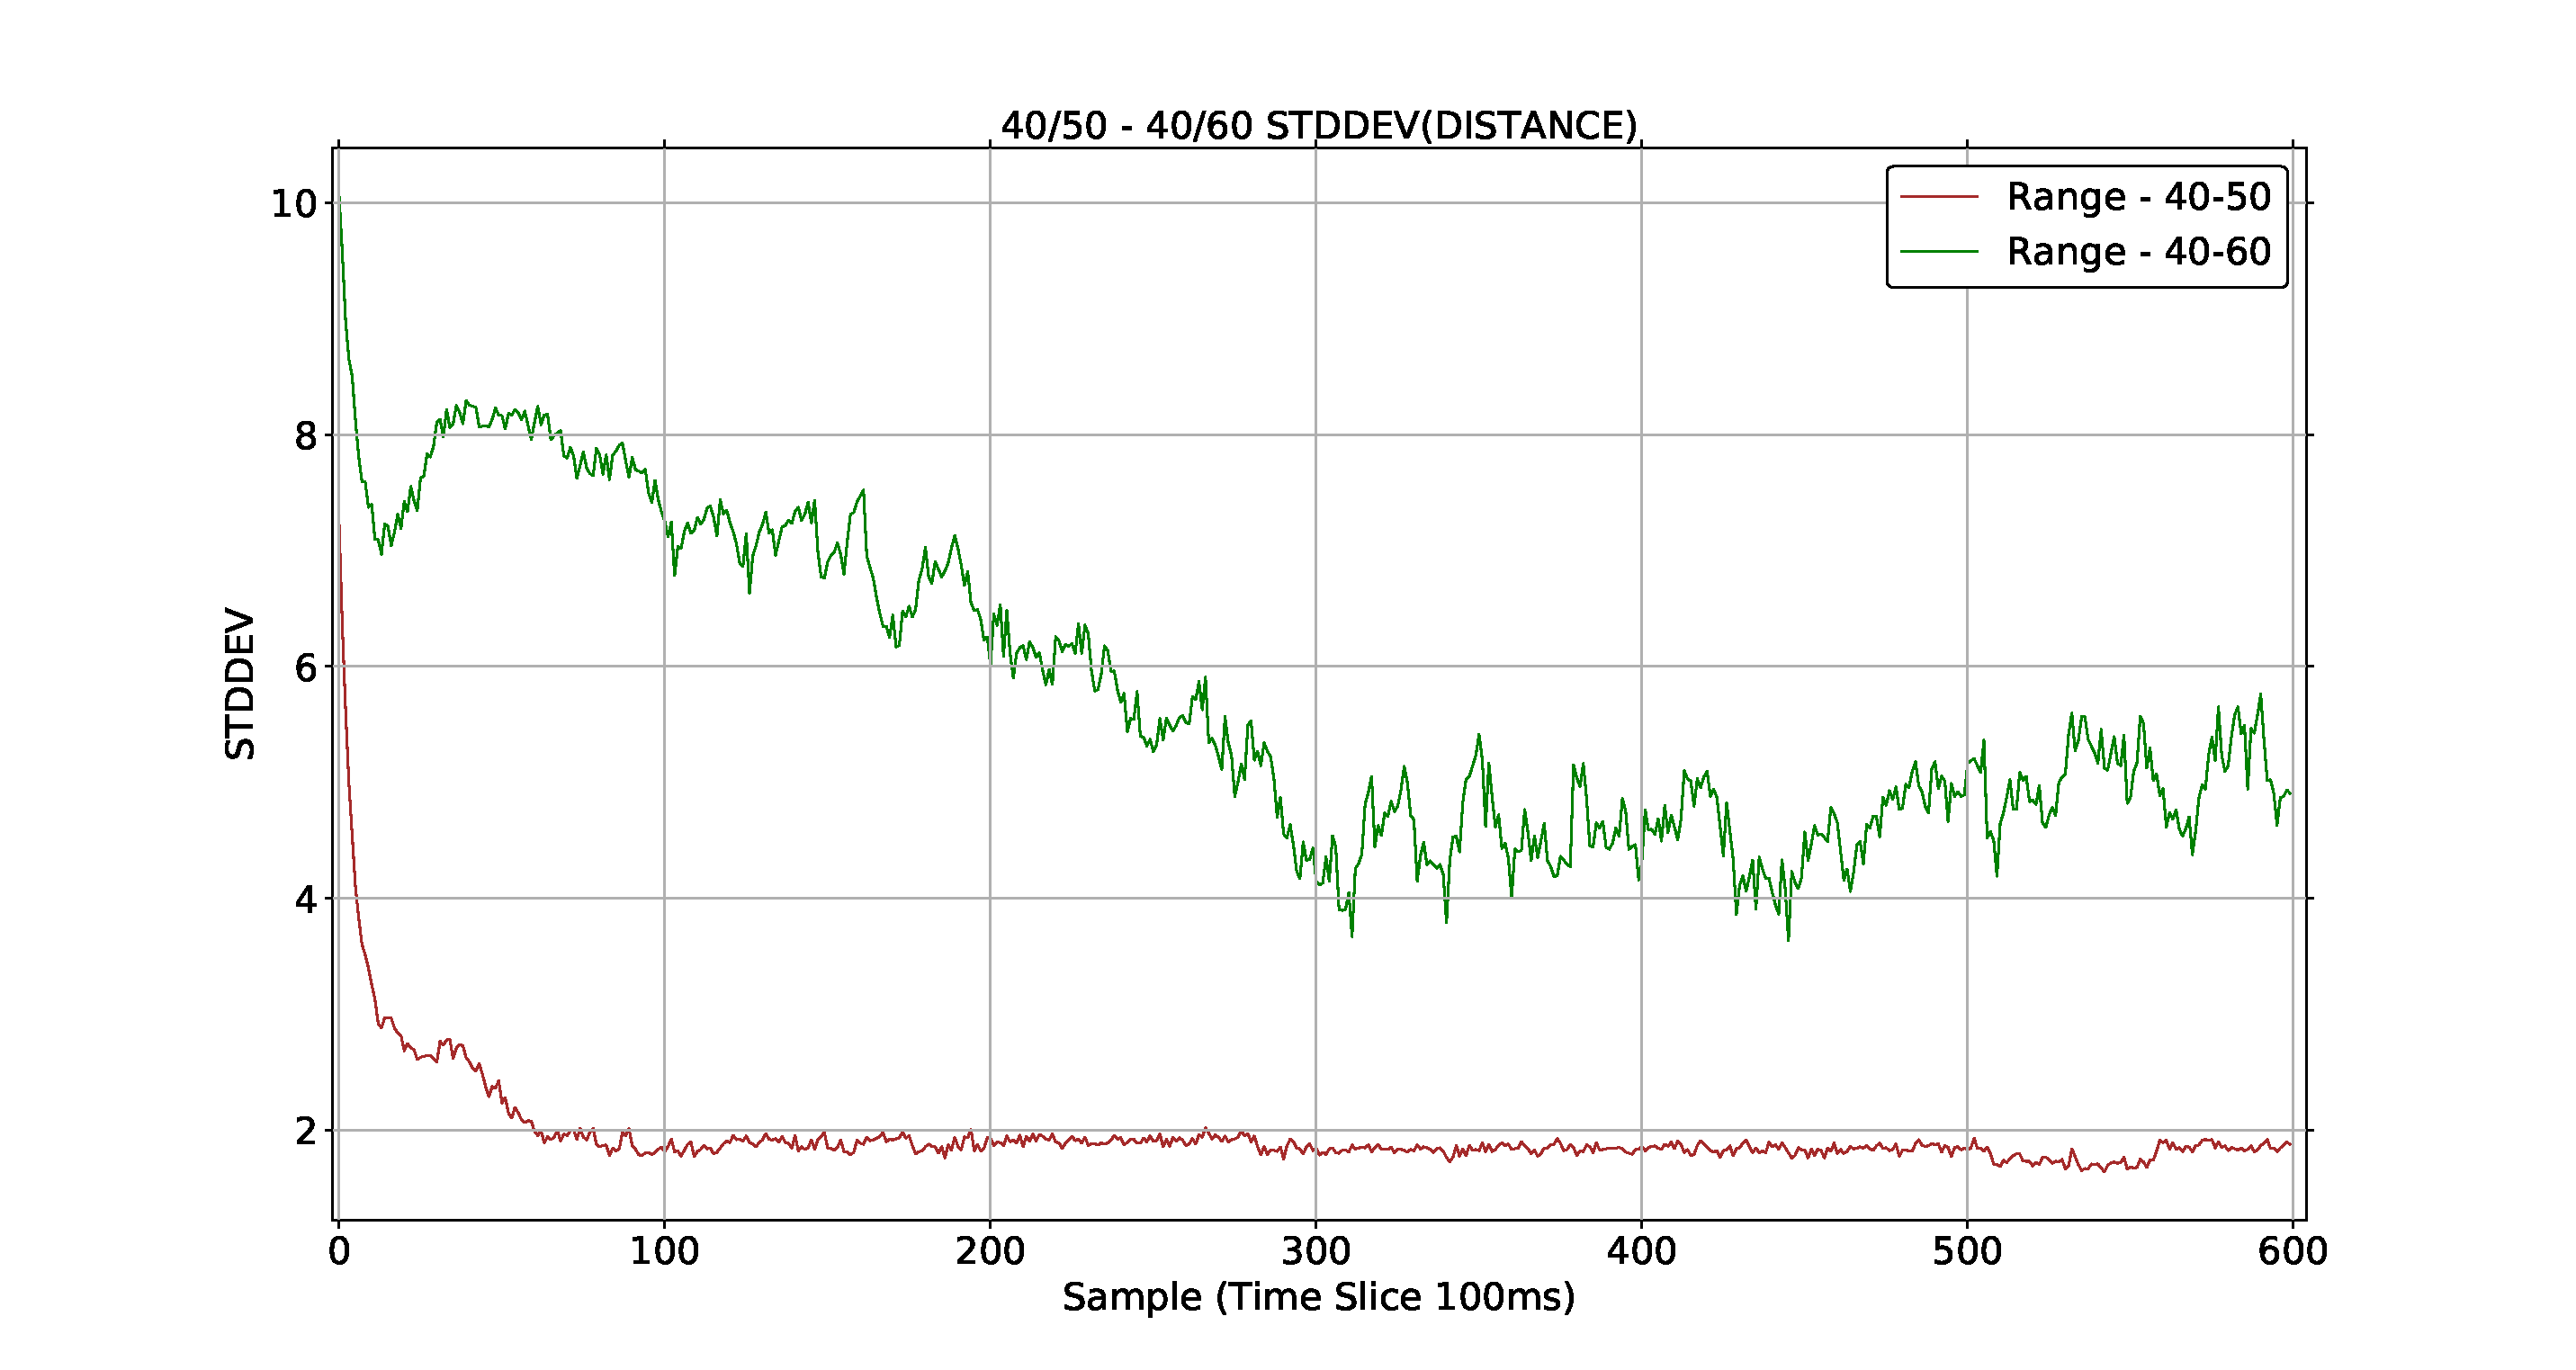
\includegraphics[width=13cm]{CHAPTER-5/figures/StabilityDistanceSwarm}
\end{center}
\caption{Distance based metric\label{methods:StabilityDistanceSwarm}}
\end{figure}
%HEX-HYPER-RES.py
\begin{figure}[H]
\begin{center}
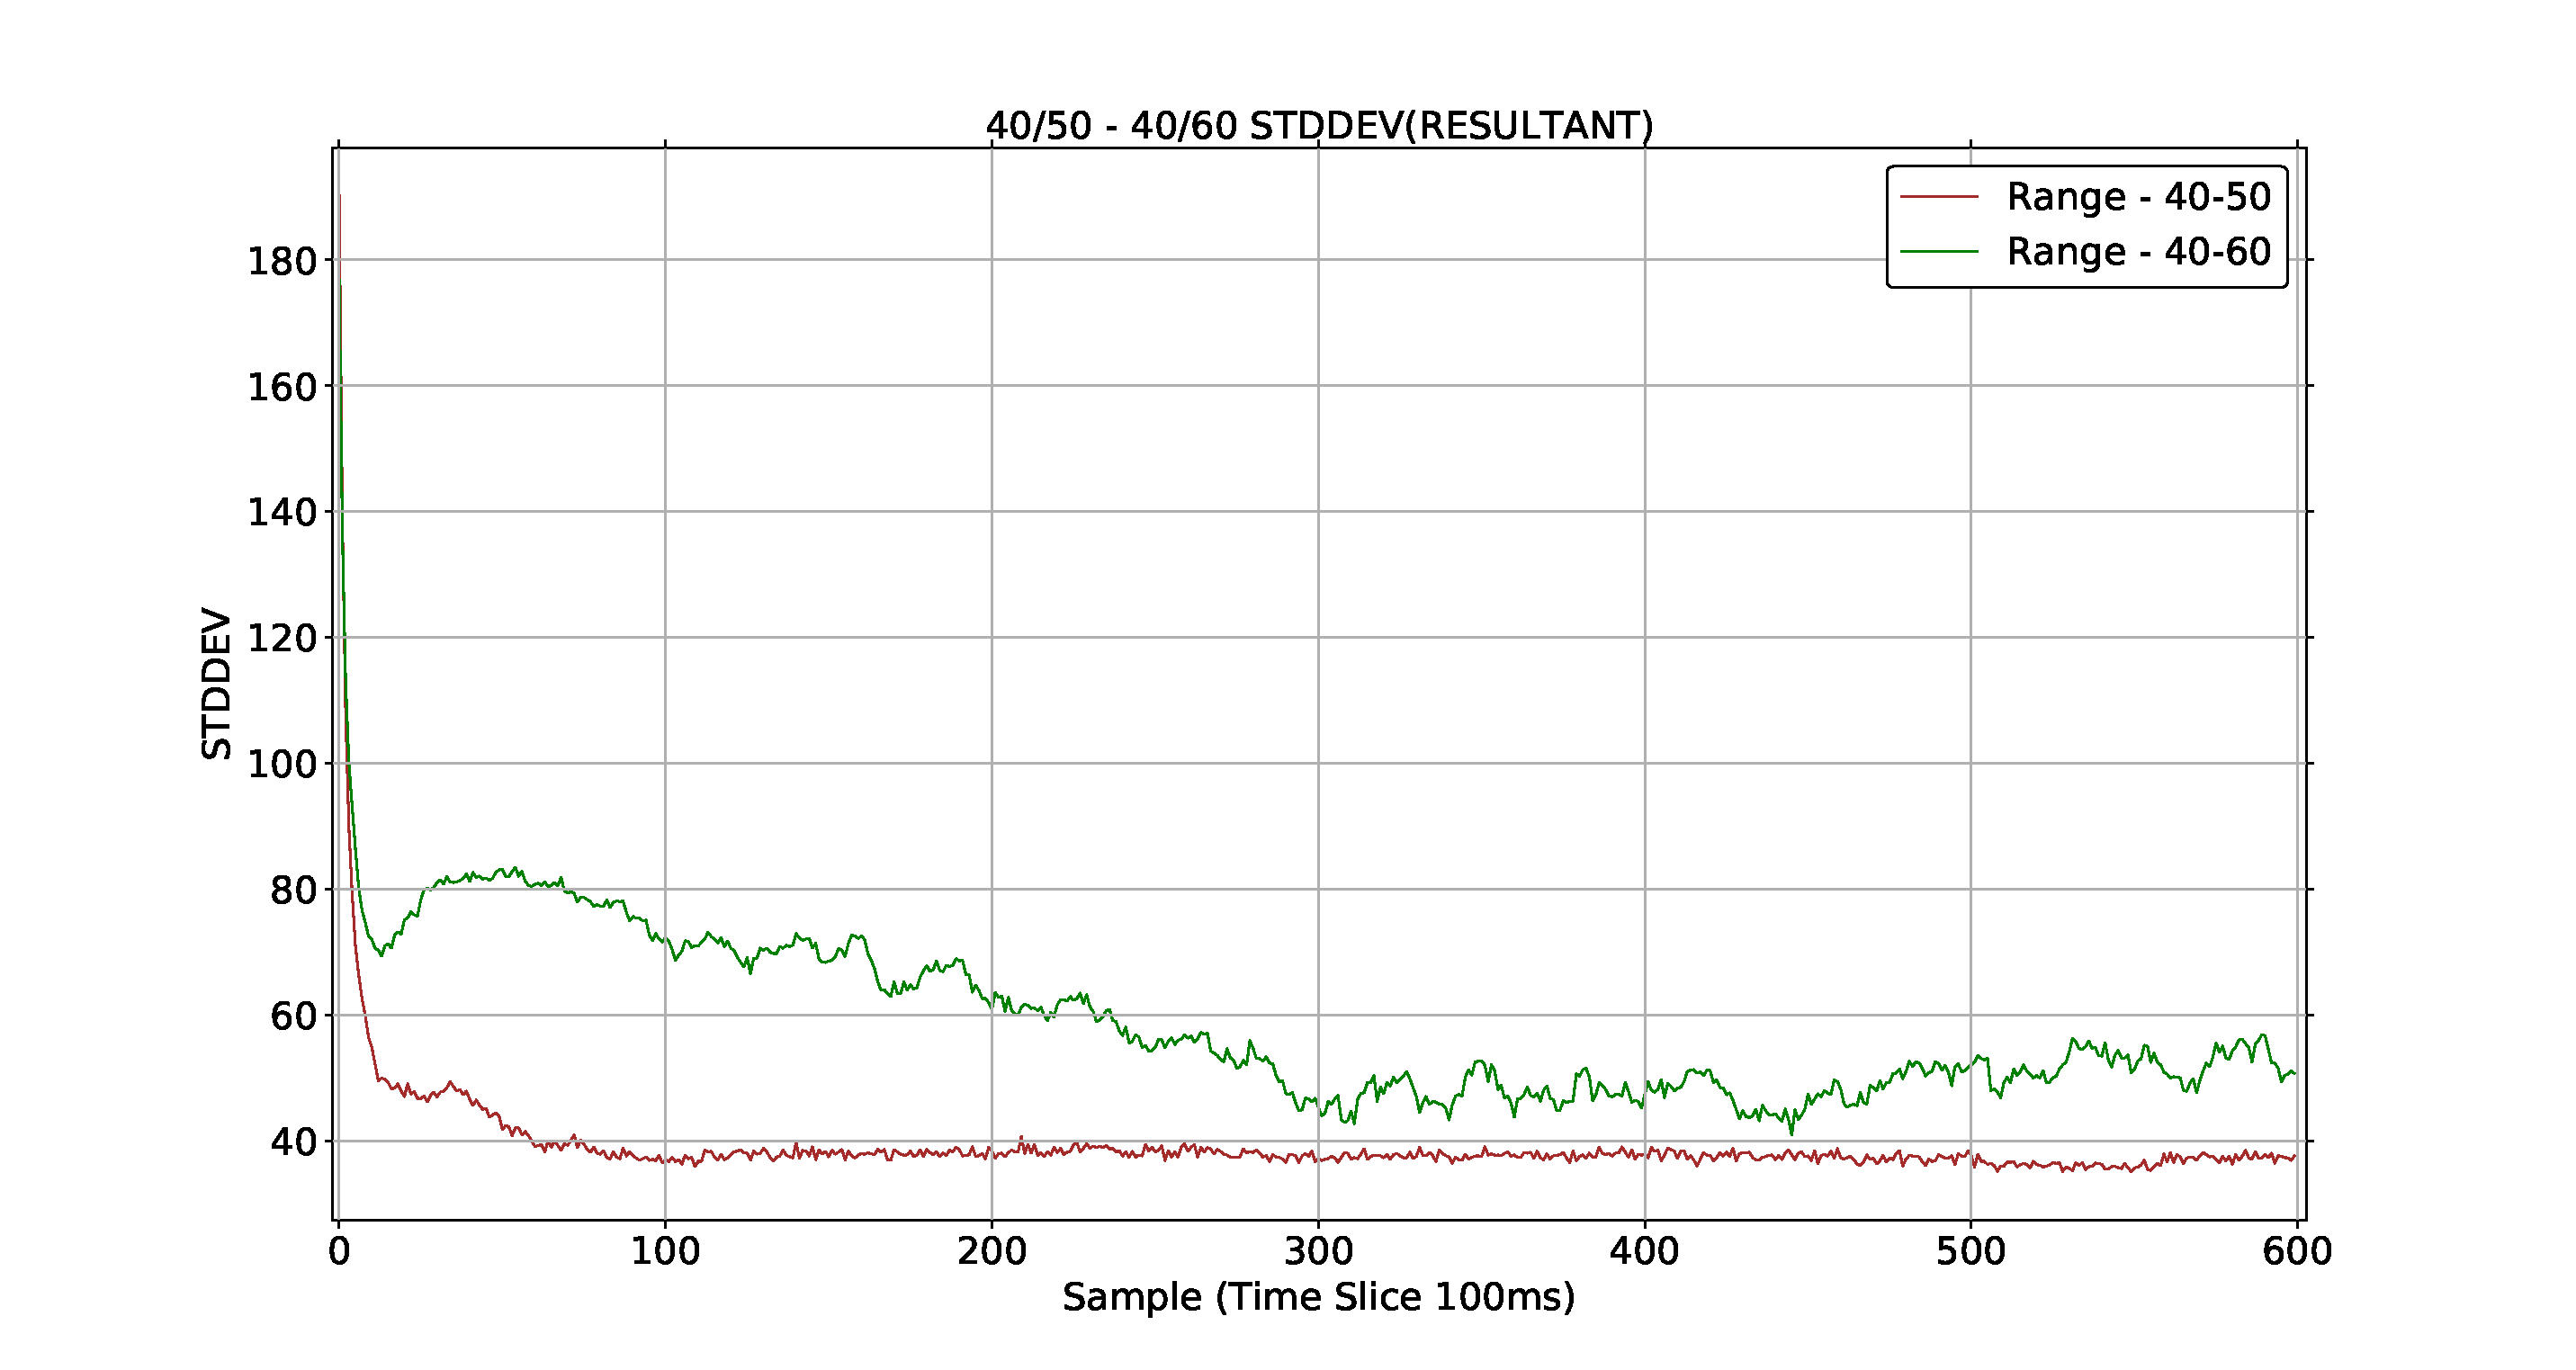
\includegraphics[width=13cm]{CHAPTER-5/figures/StabilityMagnitudeSwarm}
\end{center}
\caption{Agent resultant magnitude based metric\label{methods:StabilityMagnitudeSwarm}}
\end{figure}

The distribution of the agents over the entire simulation also shows it is possible to identify the mode of the swarm that is being generated by the cohesion field effect of the swarm. 
%HEX-HYPER-DIST-BAR.py
\begin{figure}[H]
\begin{center}
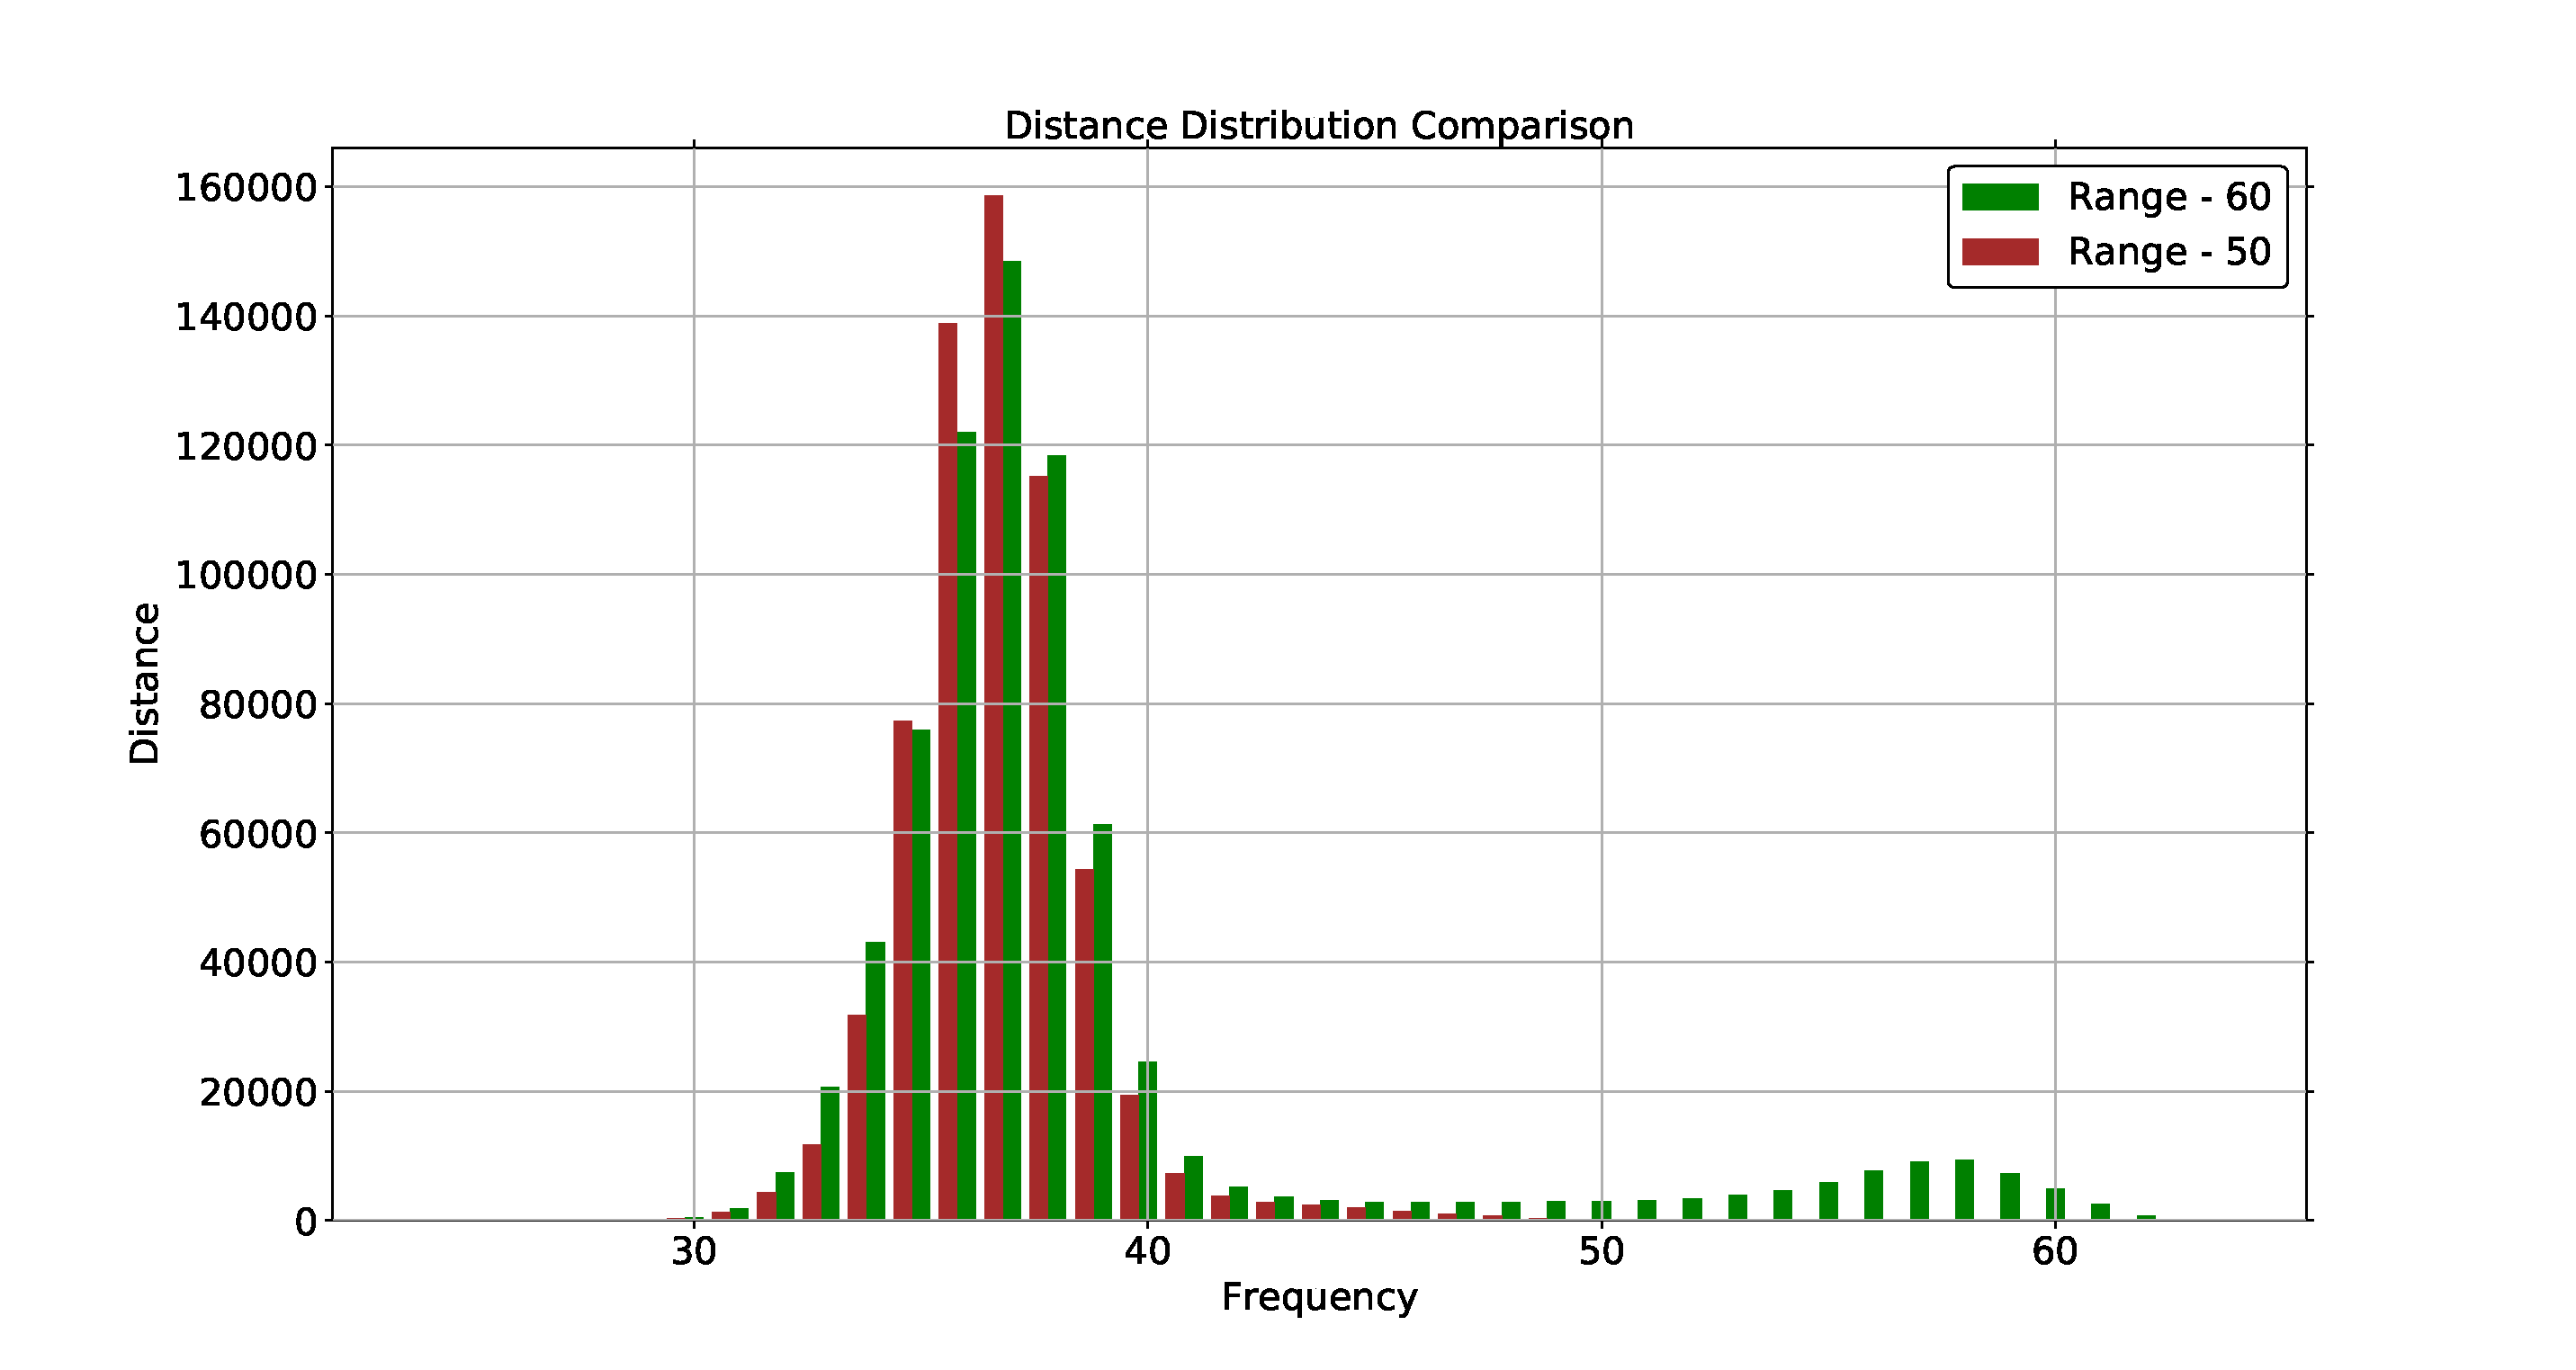
\includegraphics[width=13cm]{CHAPTER-5/figures/DistanceDistributionComparison}
\end{center}
\caption{Distance comparison\label{methods:DistanceDistributionComparison}}
\end{figure}

\autoref{methods:StabilityDistributionHyperHexagonal3D} and \ref{methods:StabilityDistributionHyperHexagonal3D2} show that over the duration of the simulation that the frequency of the mean for a hexagonal swarm is greater than that of the bi-model swarm. This is expected due to the additional vectors that are generated between agents. 
%HEX-HYPER-DIST-BAR-3D.py
\begin{figure}[H]
\begin{center}
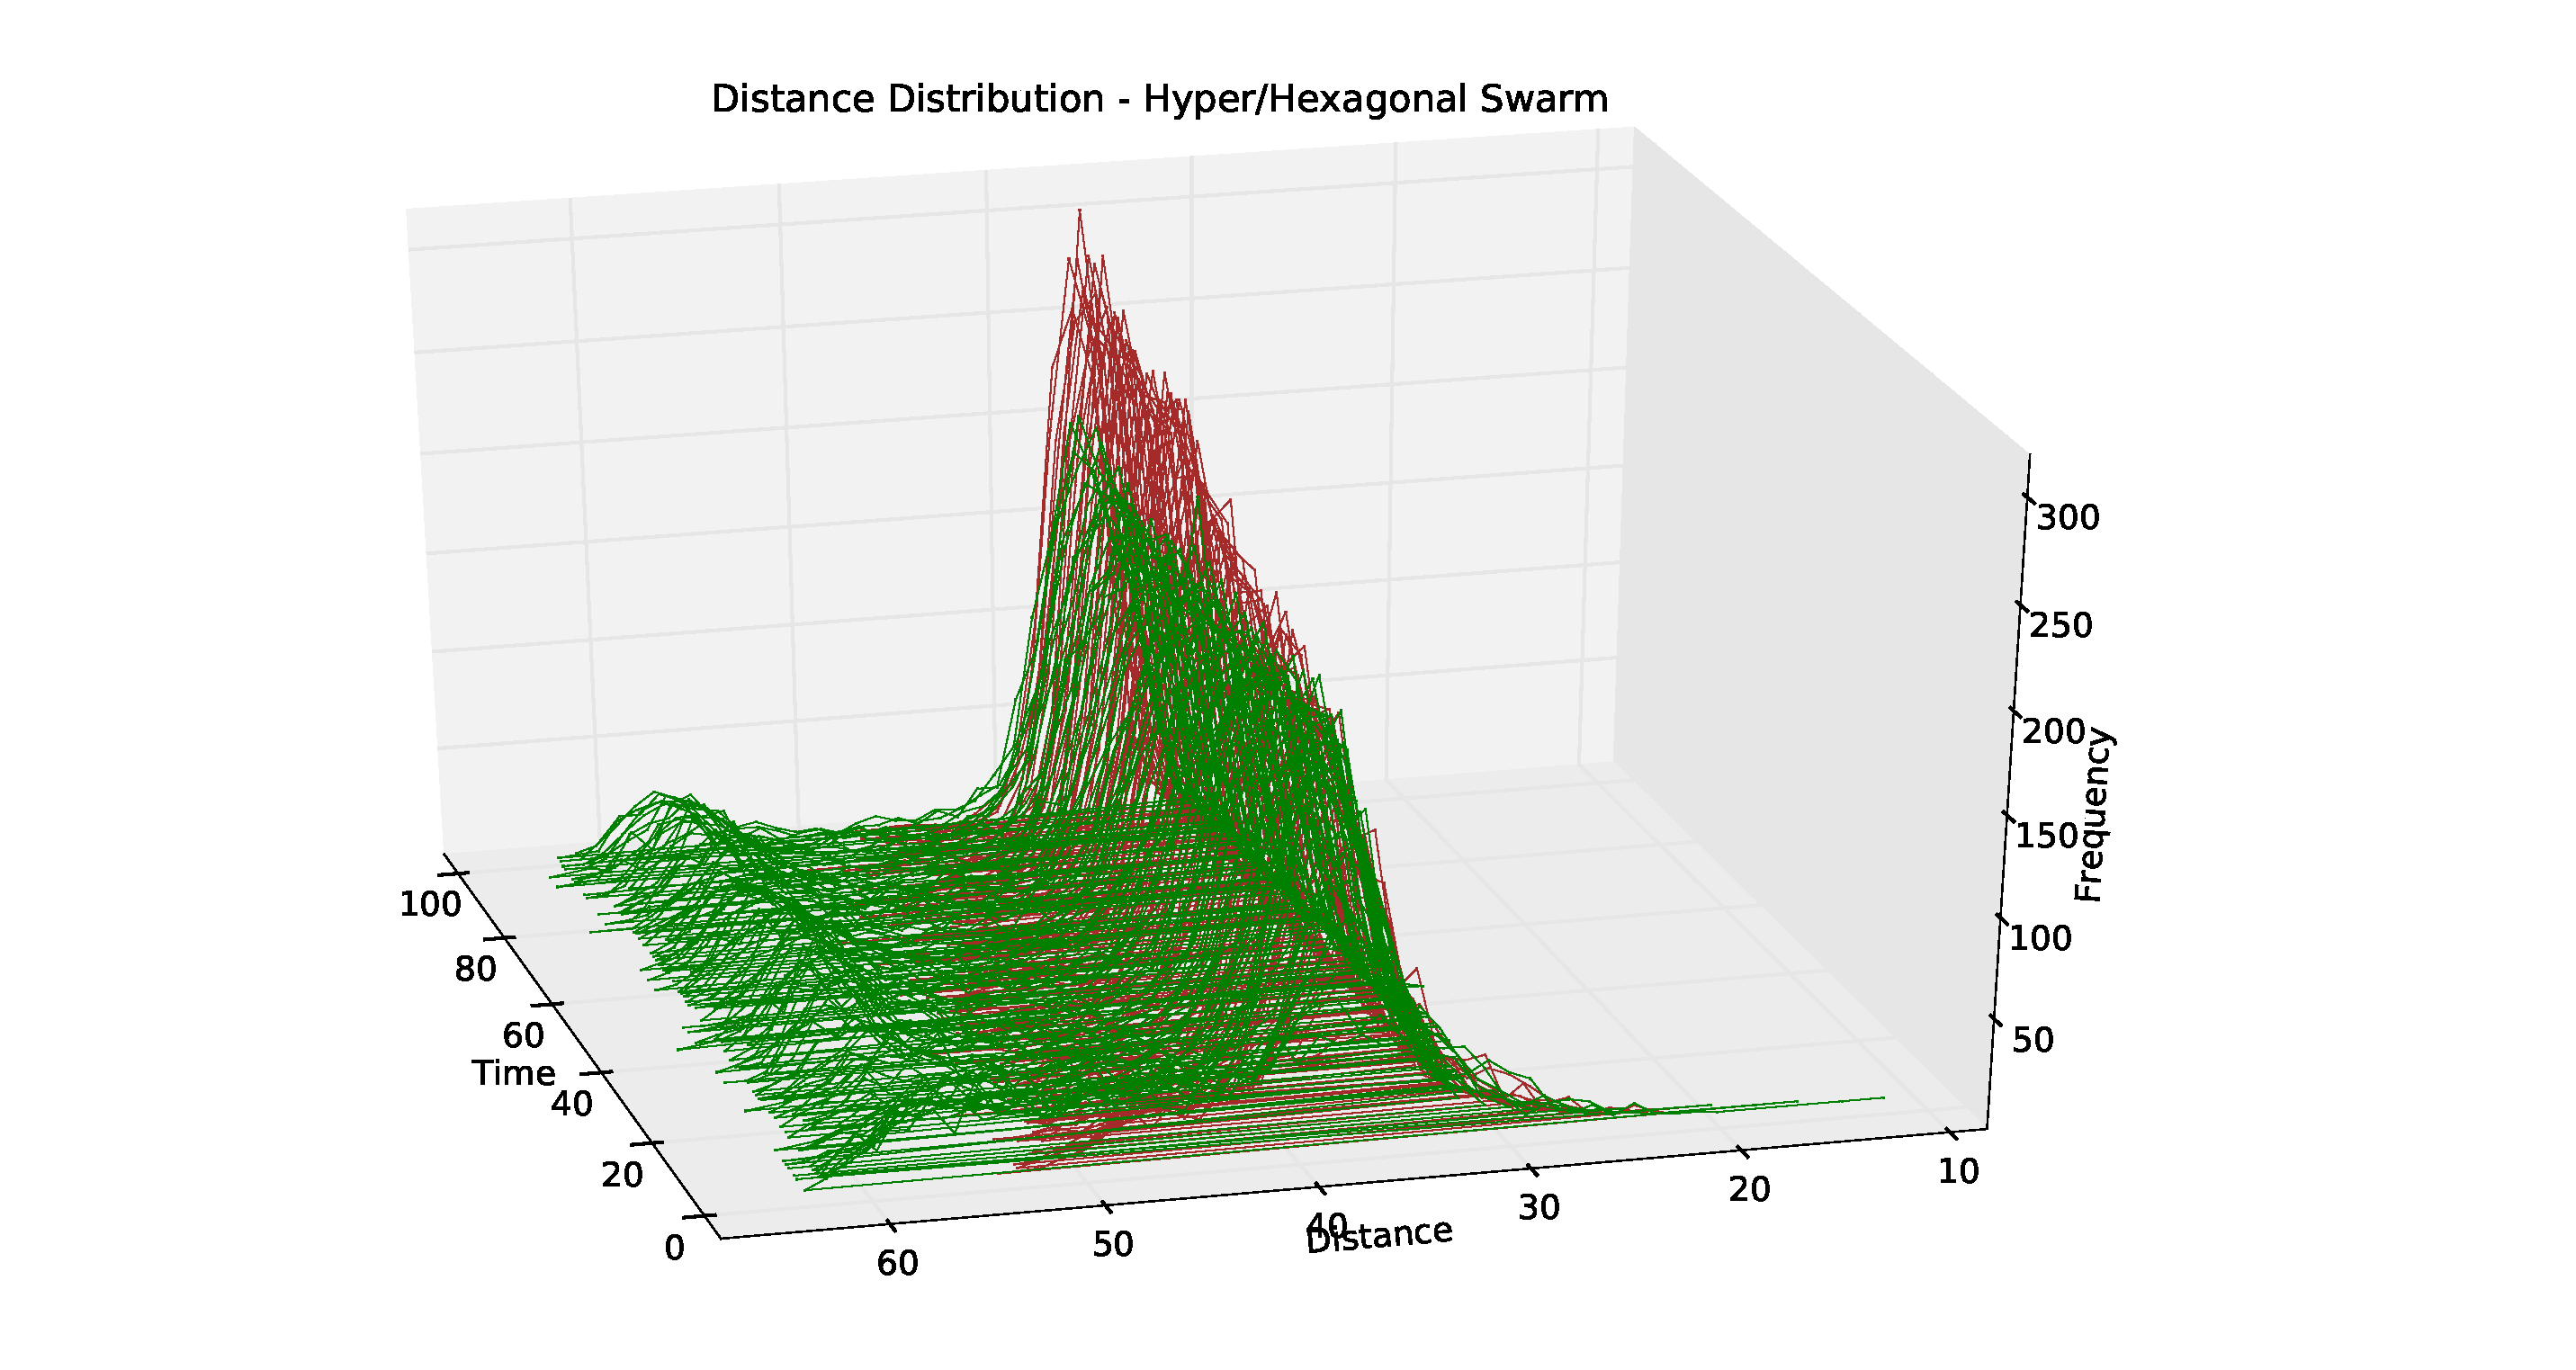
\includegraphics[width=13cm]{CHAPTER-5/figures/StabilityDistibutionHyperHexagonal3D}
\end{center}
\caption{Distance comparison / Time 0-10 seconds\label{methods:StabilityDistributionHyperHexagonal3D}}
\end{figure}
%HEX-HYPER-DIST-BAR-3D.py
\begin{figure}[H]
\begin{center}
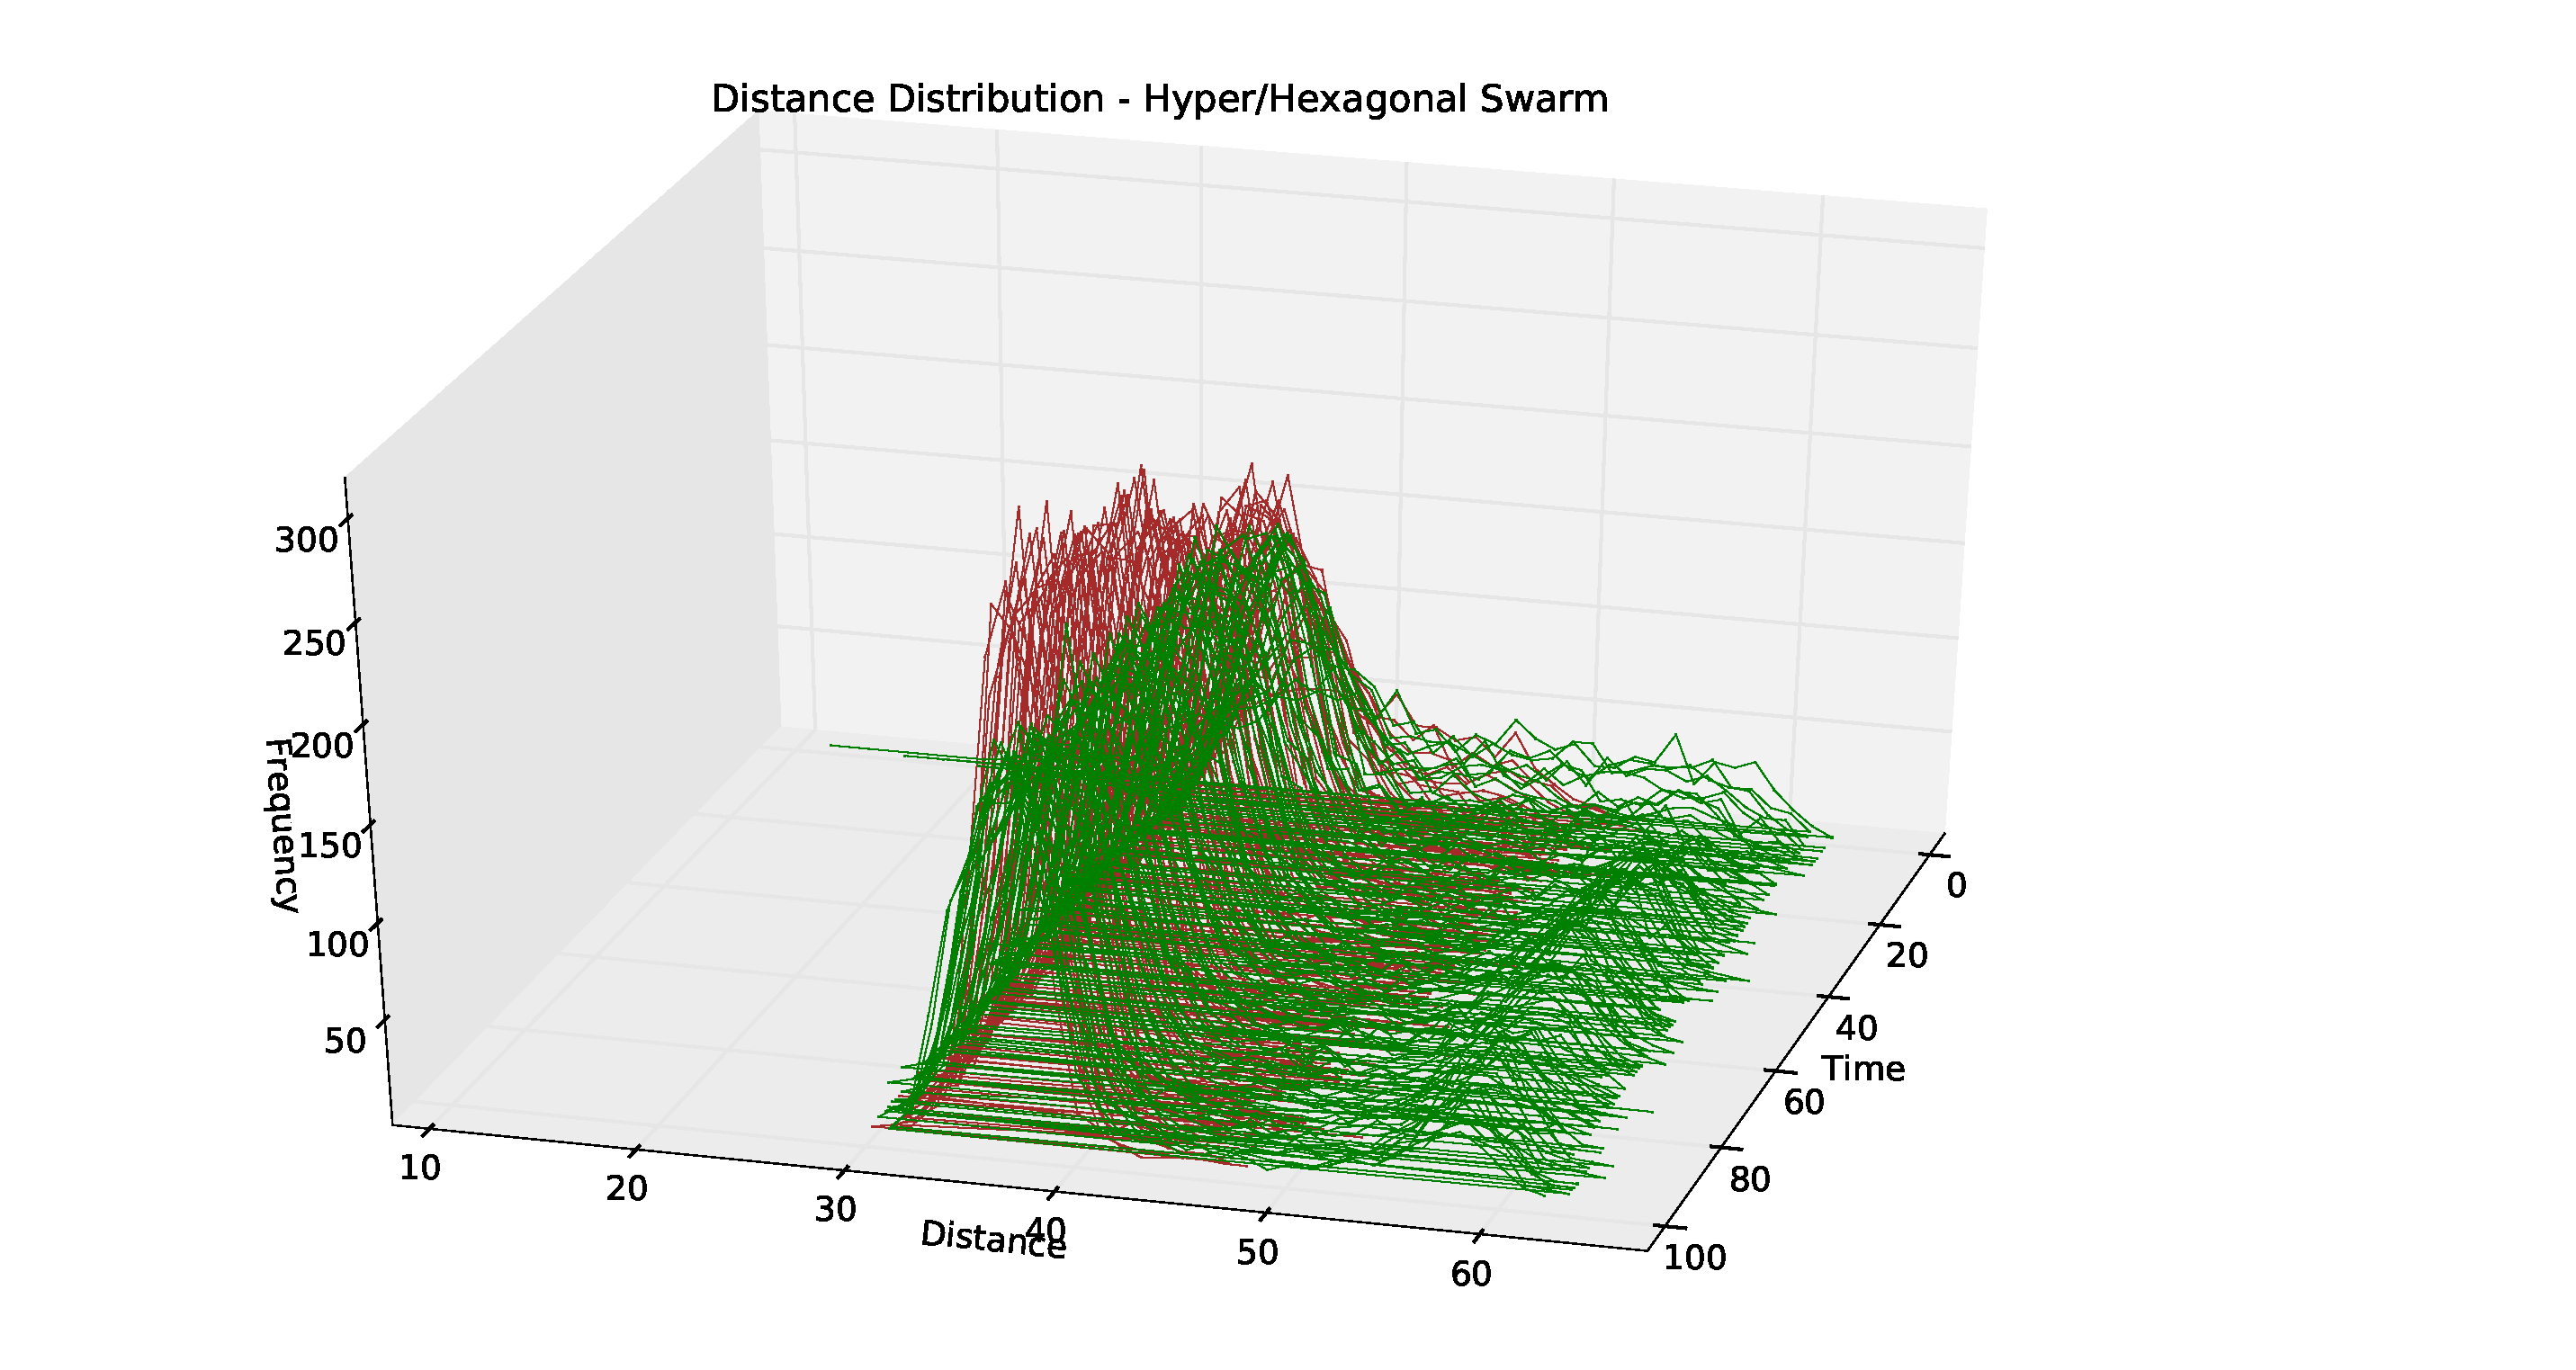
\includegraphics[width=13cm]{CHAPTER-5/figures/StabilityDistibutionHyperHexagonal3D2}
\end{center}
\caption{Distance comparison / Time 10-0 seconds\label{methods:StabilityDistributionHyperHexagonal3D2}}
\end{figure}

\autoref{methods:MagnitudeDistributionComparison} shows that the mean magnitude potential for a hexagonal swarm is lower than that of the hyper-connected swarm.
%HEX-HYPER-MAG-BAR.py
\begin{figure}[H]
\begin{center}
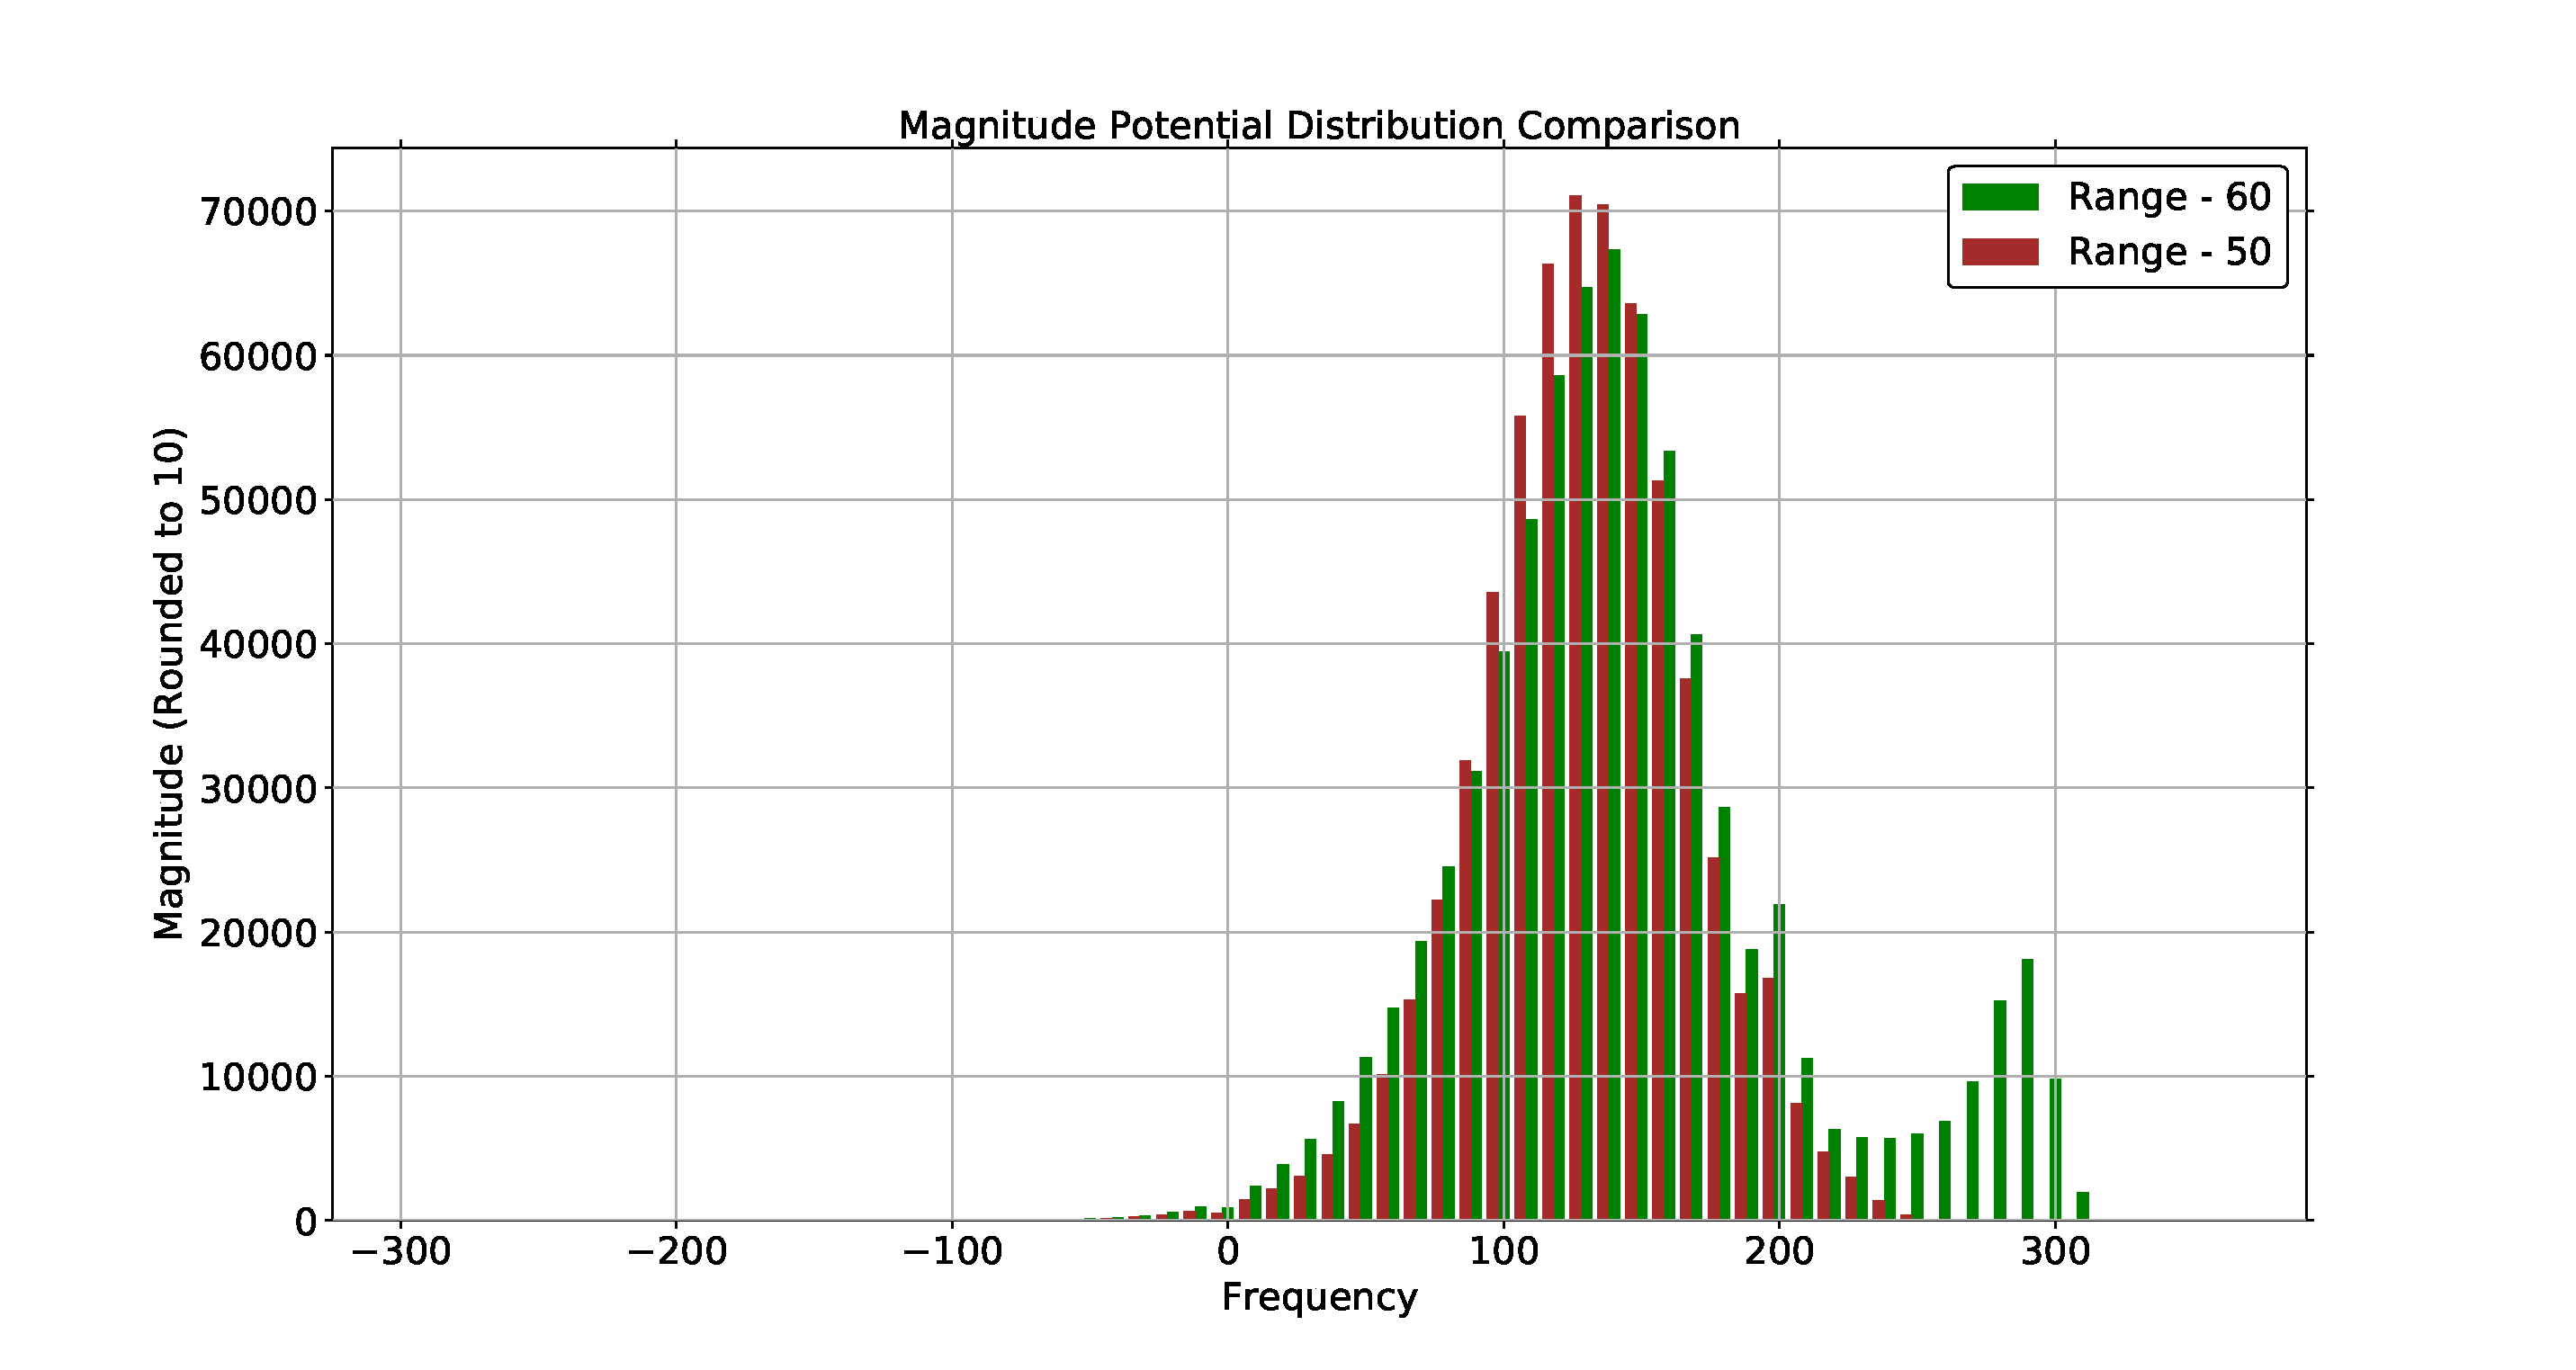
\includegraphics[width=13cm]{CHAPTER-5/figures/MagnitudeDistributionComparison}
\end{center}
\caption{Agent resultant magnitude comparison\label{methods:MagnitudeDistributionComparison}}
\end{figure}

The most notable difference between the two magnitude metric analyses (\autoref{methods:StabilityMagHyperHexagonal3D} and \ref{methods:StabilityMagHyperHexagonal3D2}) is the initial potential magnitude of the hyper-connected swarm being greater than the hexagonal-swarm. This is due to the additional range of the field effect which generates a larger initial magnitude potential drawing the swarm together.
%HYPER-HEX-MAG-BAR-3D.py
\begin{figure}[H]
\begin{center}
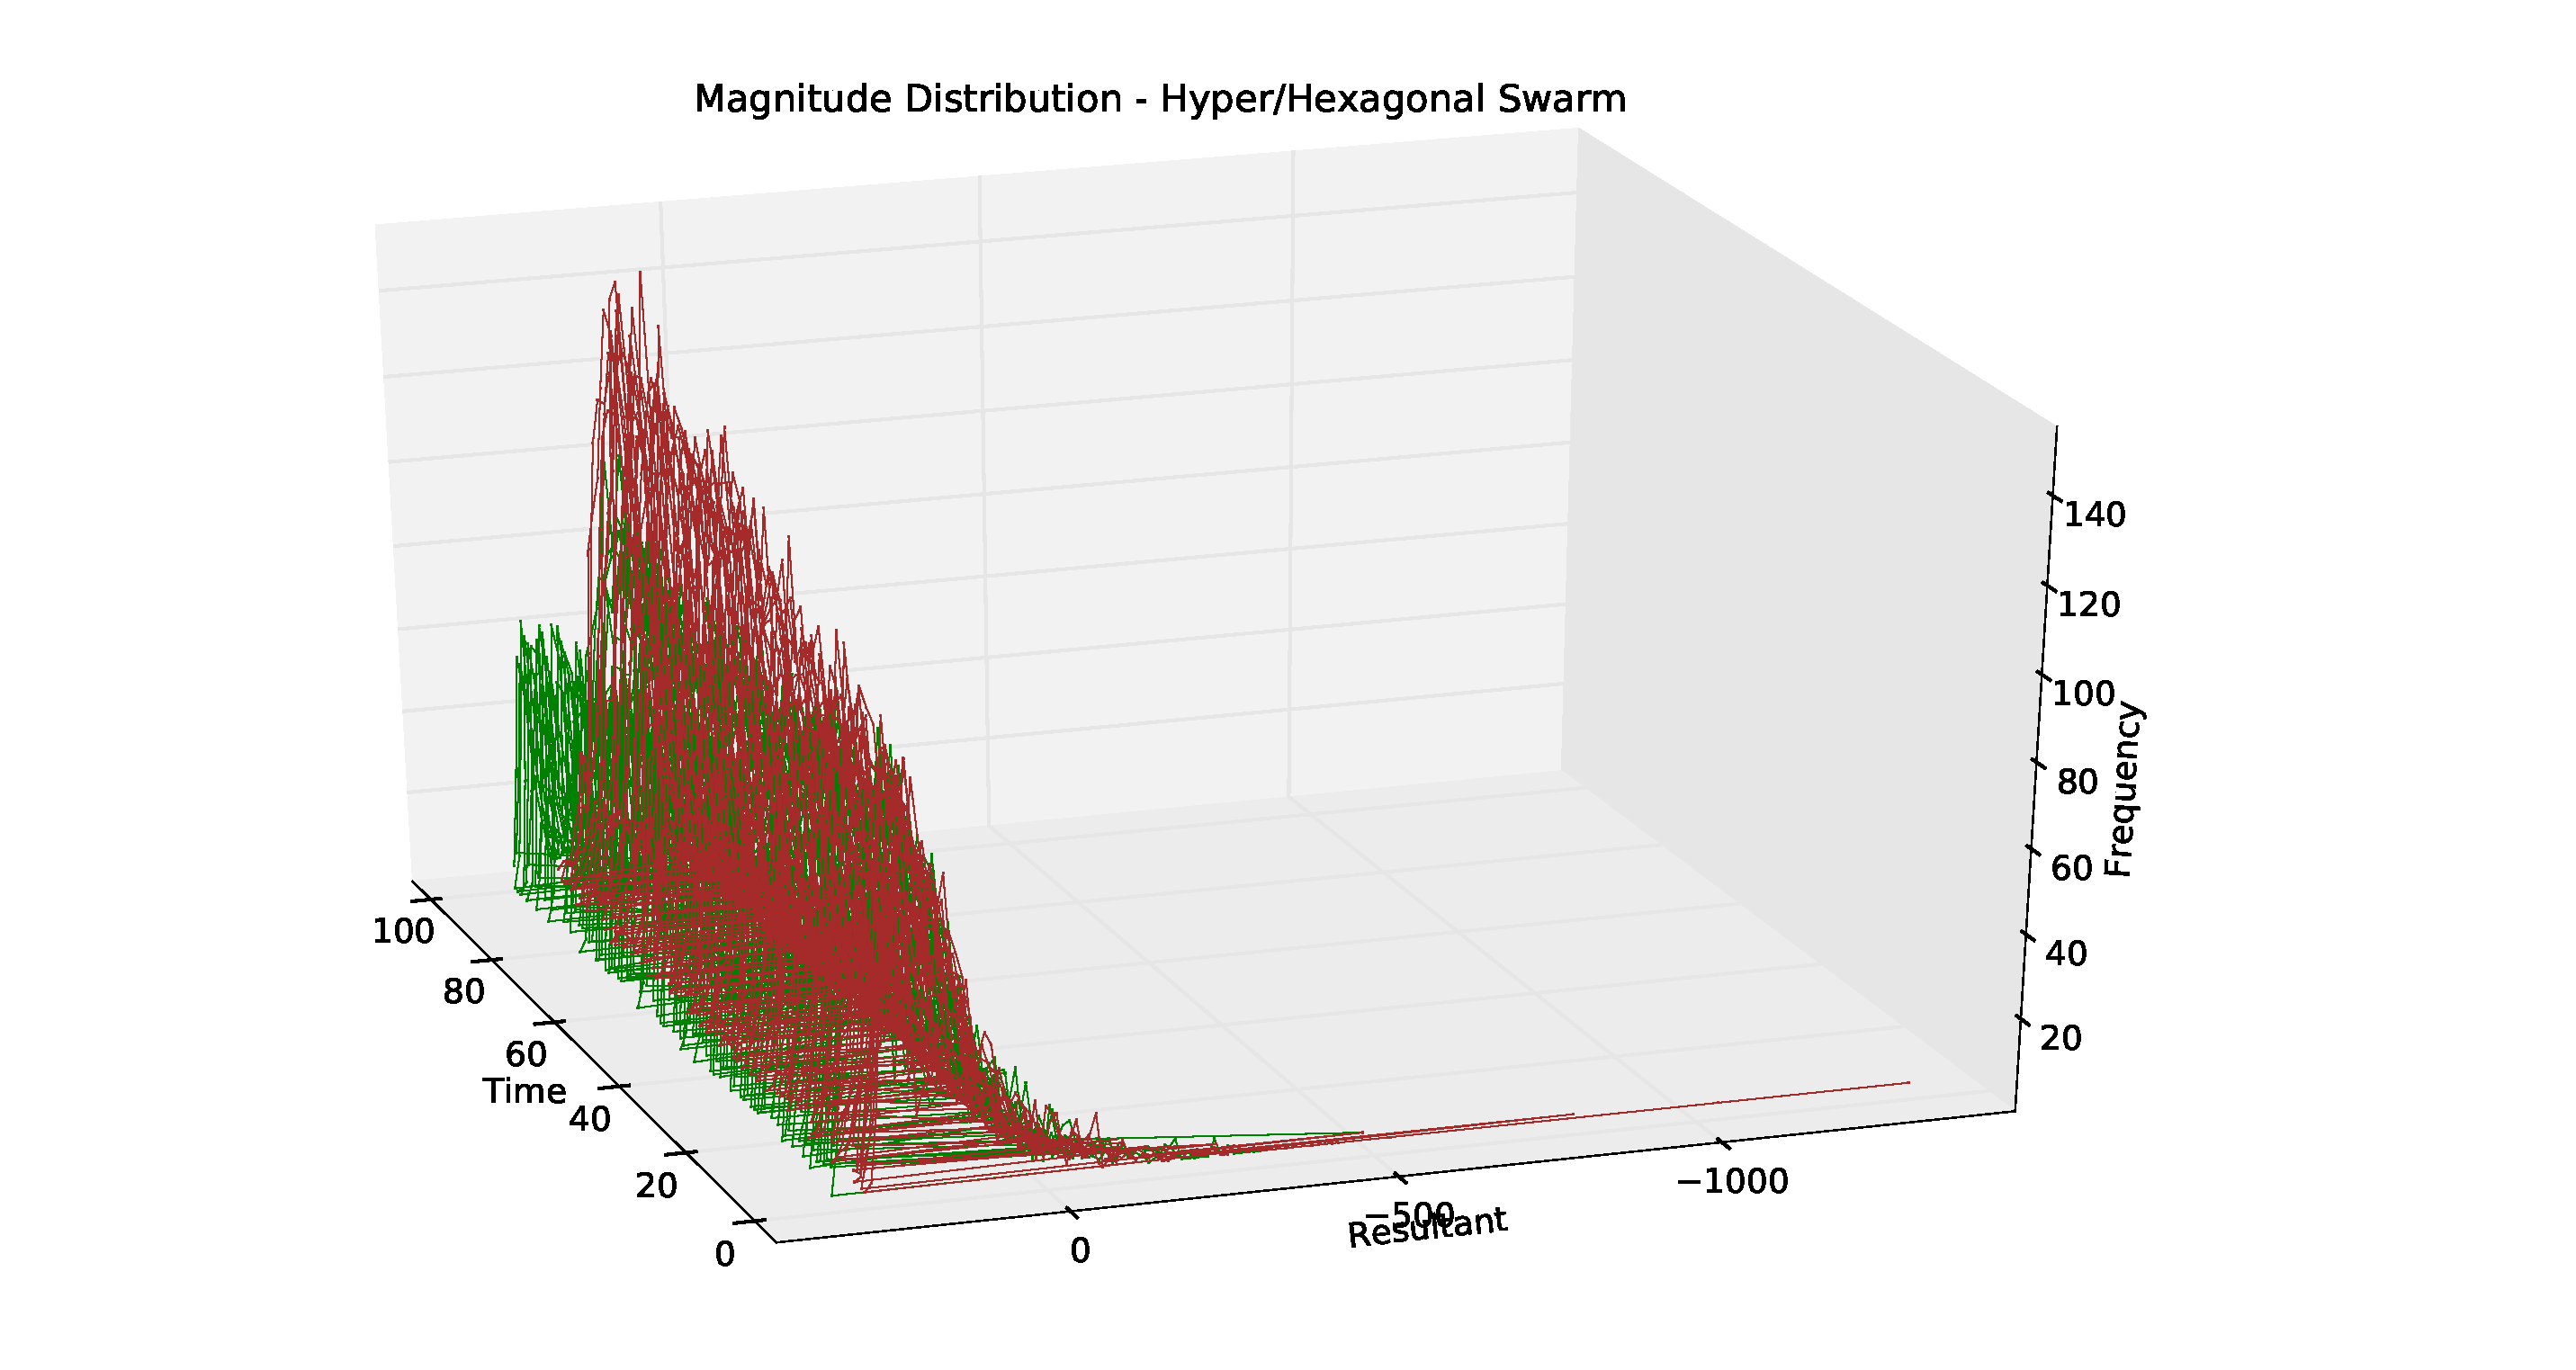
\includegraphics[width=13cm]{CHAPTER-5/figures/StabilityMagHyperHexagonal3D}
\end{center}
\caption{Agent resultant magnitude comparison / Time 0-10 seconds\label{methods:StabilityMagHyperHexagonal3D}}
\end{figure}

\begin{figure}[H]
\begin{center}
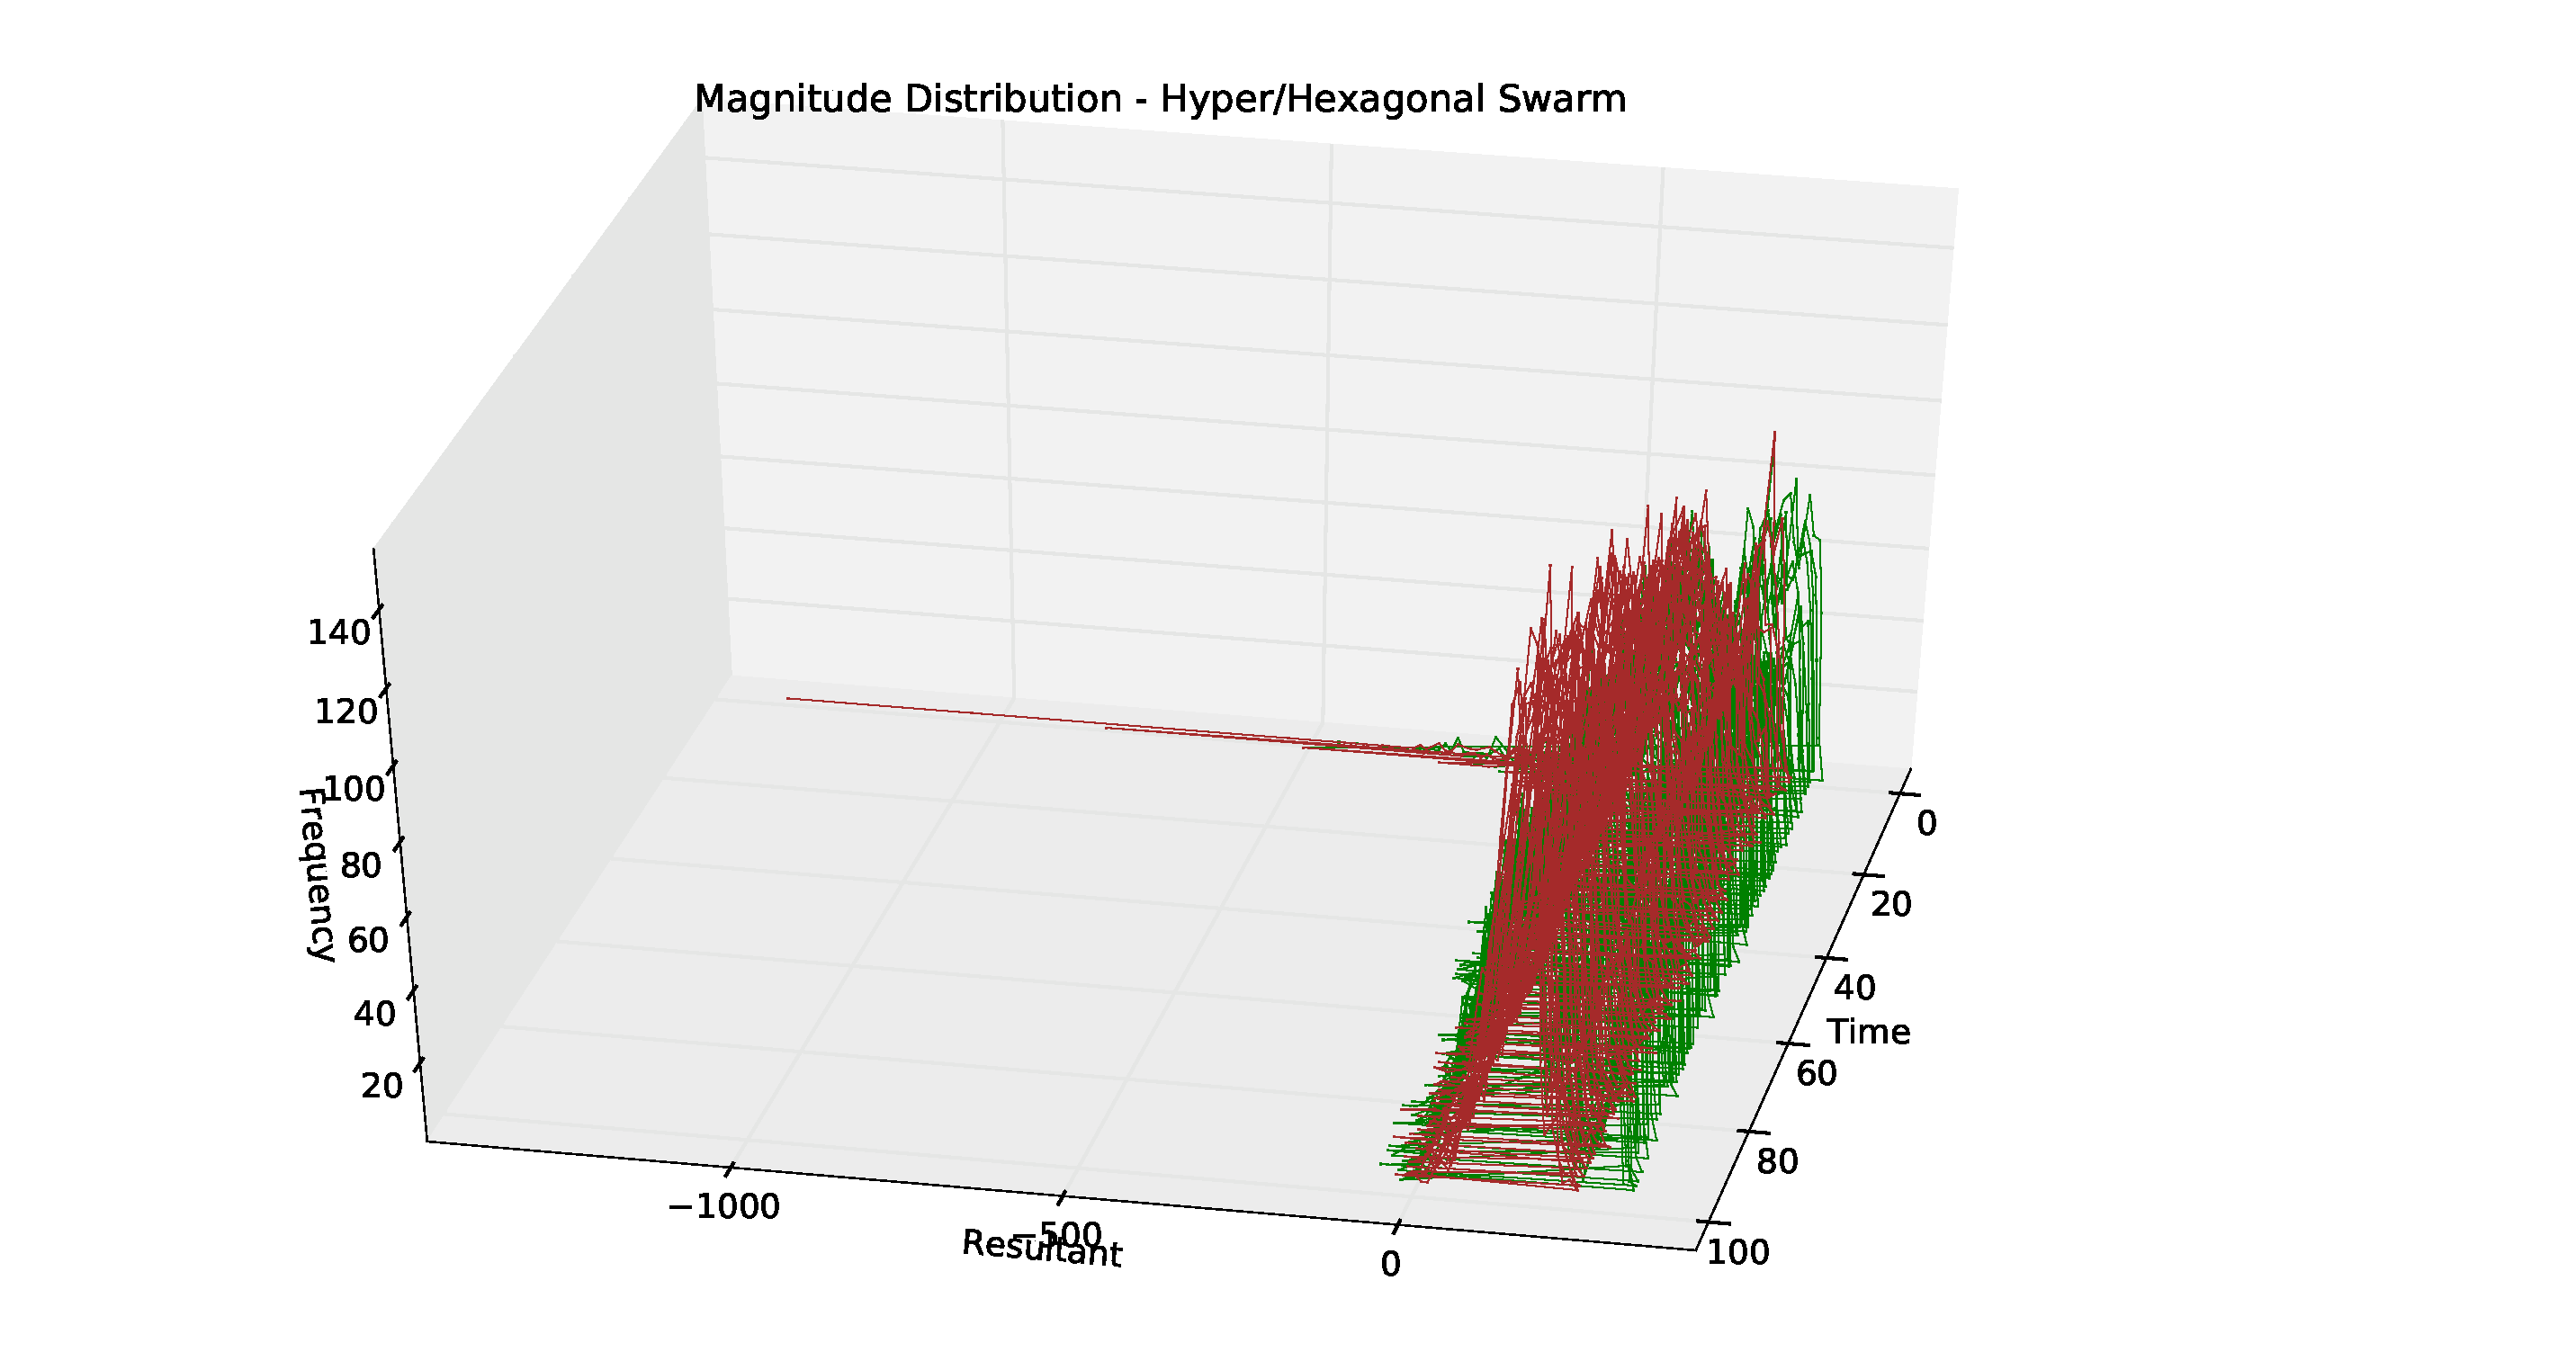
\includegraphics[width=13cm]{CHAPTER-5/figures/StabilityMagHyperHexagonal3D2}
\end{center}
\caption{Agent resultant magnitude comparison / Time 10-0s\label{methods:StabilityMagHyperHexagonal3D2}}
\end{figure}

\section{Static swarm conclusion\label{section:staticConclusion}}
These results in terms of using magnitude or distance, provide similar profiles in terms of the changes in the profile of the plotted results. The distance metric discussed by Navarro~\cite{NIM:09} is used by many researchers that analyse agent distribution such as Cheein et al.~\cite{HGCTREA:15}, Bennet et al.~\cite{BM:09} and Barnes et al.~\cite{BAF:06, BAFVM:06, BFV:07, BFV:09}. Gazi et al.~\cite{GP:02, GP:04, GP:04a, GP:05} use this metric to analyse swarm stability. 

The similar profiles of the two metrics shows that either mechanism is suitable for identifying the internal movement within the swarm and providing a mechanism to compare the effects of swarming algorithms. The magnitude analysis, however, also provides a mechanism to determine if the swarm is expanding (a negative magnitude) or cohesive (a positive magnitude).

The metrics both provide an ability to adjust the variable parameters of the swarming mechanics (cohesion, repulsion and direction) or the range of the neighbour detection and minimum proximity distances and to identify the effect that those changes have upon the swarm in terms of the swarm's internal movement. If we consider the internal movement to be a measure of the quality of a swarm in a given situation then these measures are identifying the swarming algorithms effectiveness.

\subsection{Arbitrary sized swarms}\label{section:arbitrary}
This thesis if focused on arbitrary sized swarm's. The algorithms that are used only require localised sensing which therefore all movement and positioning calculations are based on neighbours. As localised data is used it should be possible for the algorithms to be effective with swarms of any size. The swarm's configuration in this section is based upon a swarm of 200 agents but the application of the field effects coordination will work with larger swarms. \autoref{methods:ArbitrarySize200500} shows a comparison the distance metric of swarms of 200 and 500 agents and \autoref{methods:ArbitrarySizeMag200500} shows a comparison of the Magnitudes.

\begin{figure}[H]
\begin{center}
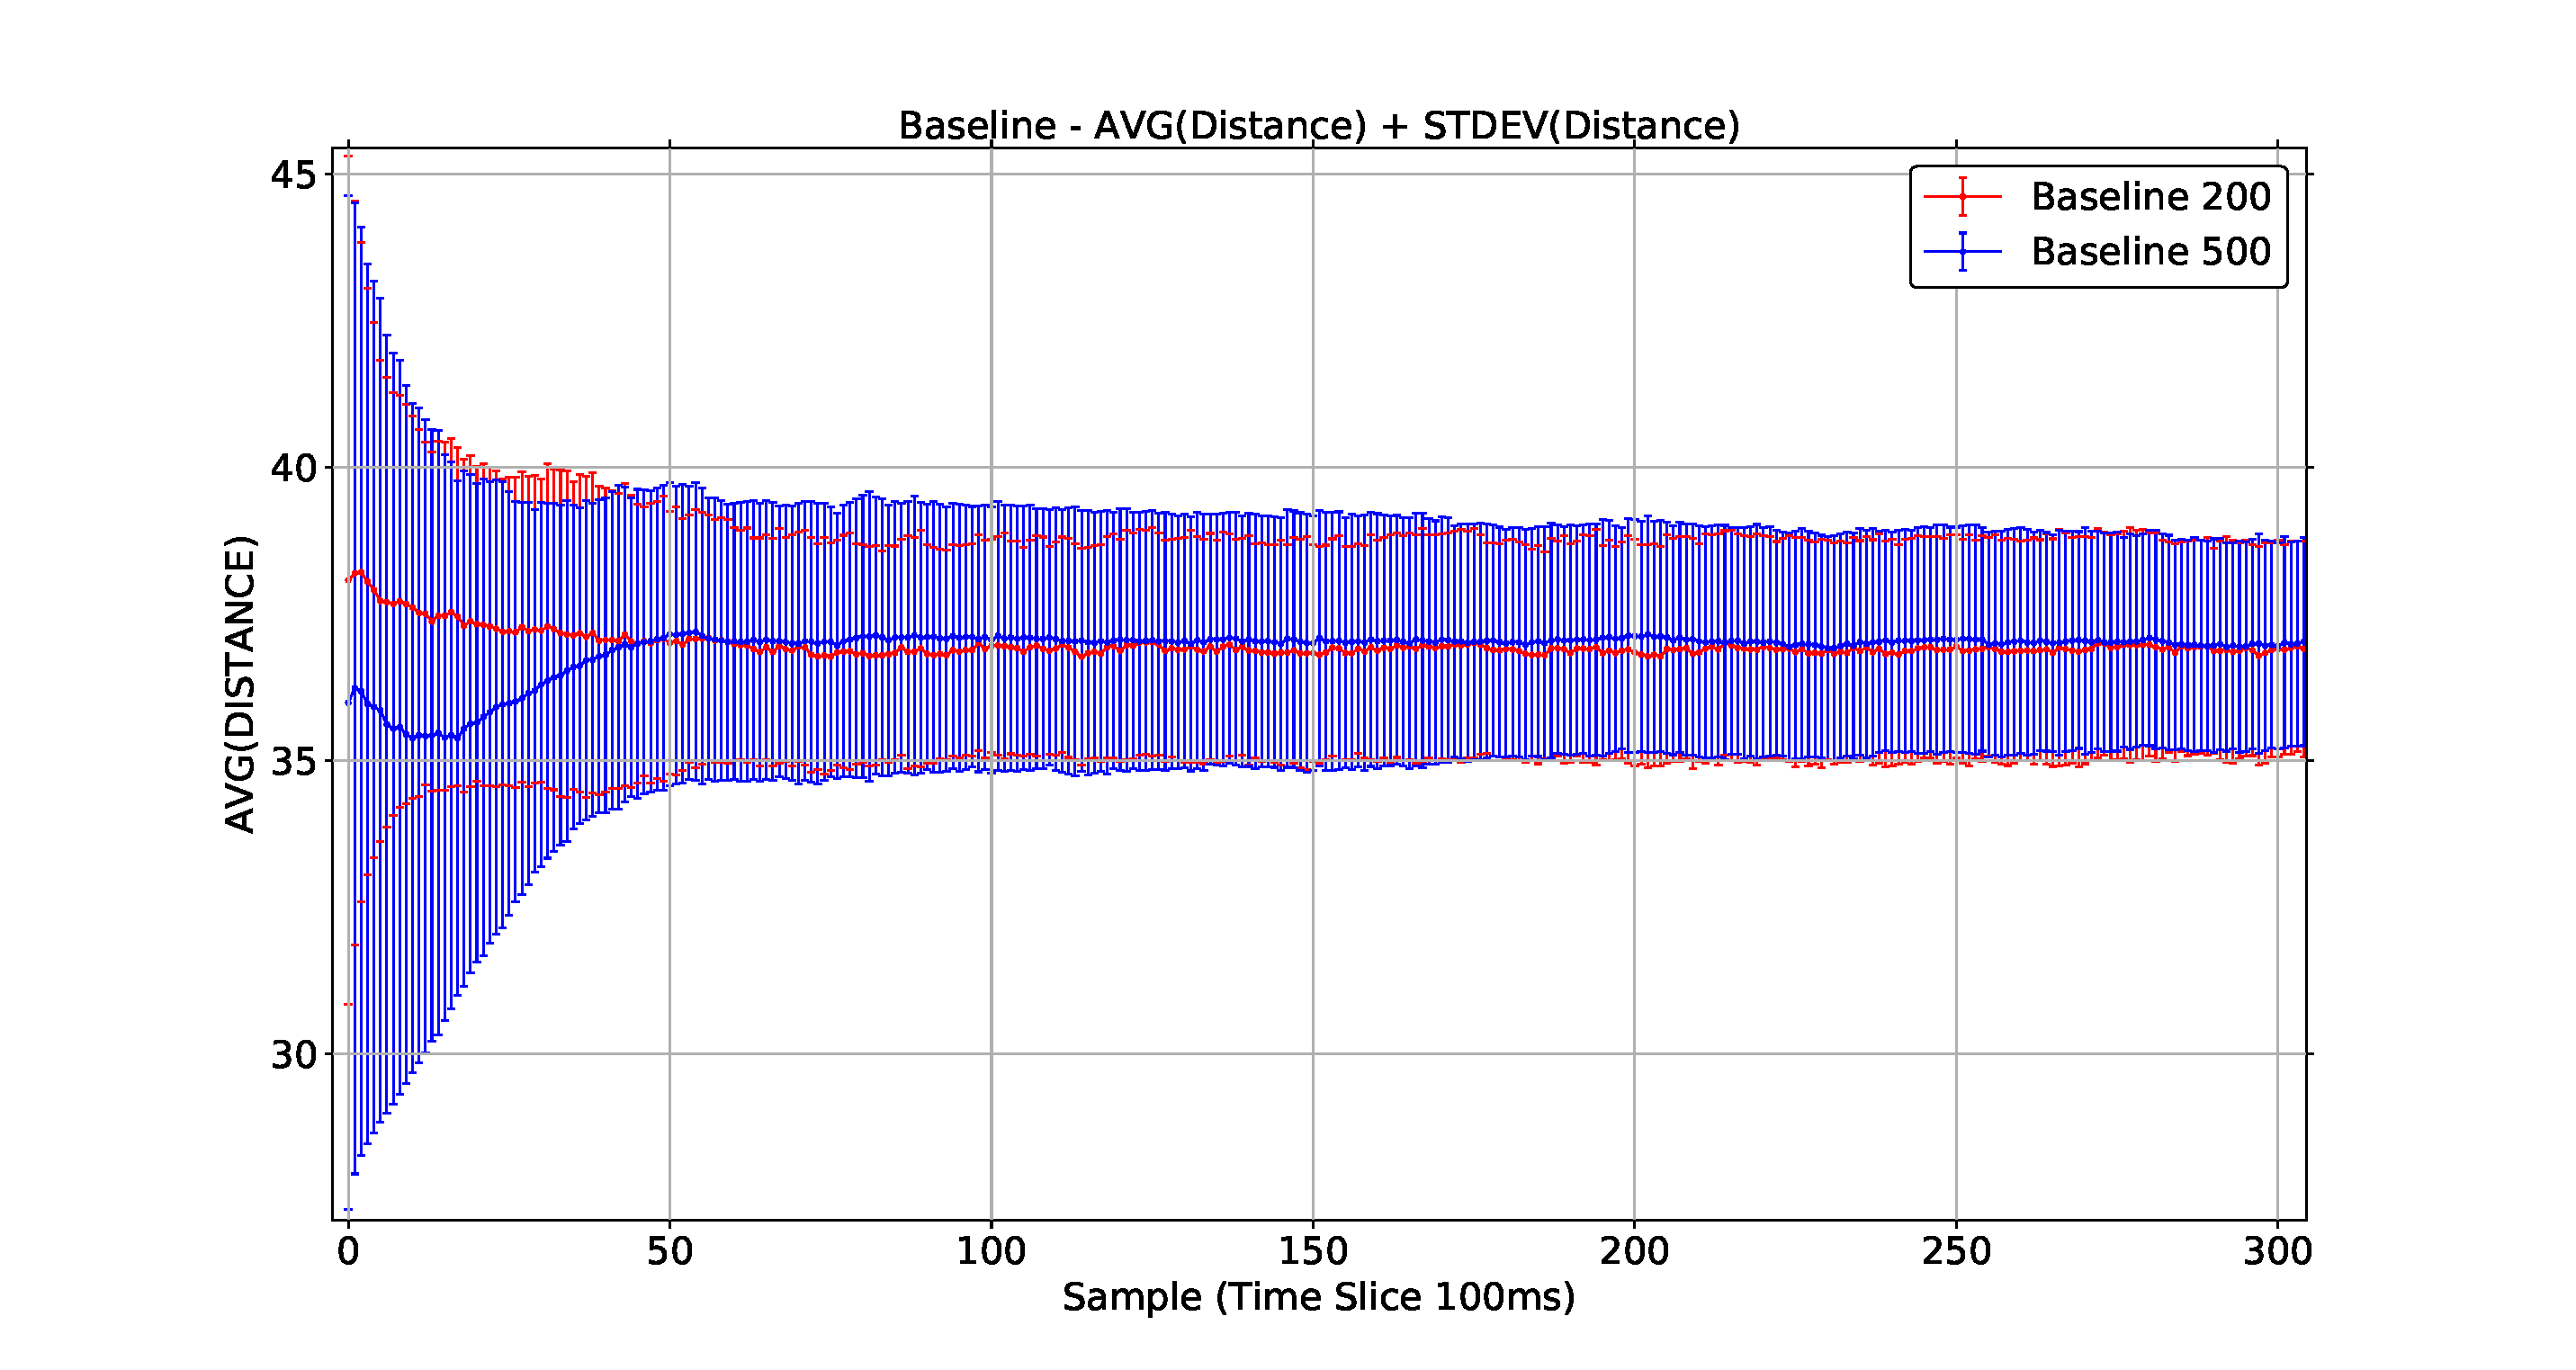
\includegraphics[width=13cm]{CHAPTER-5/figures/ArbitrarySize200500}
\end{center}
\caption{Swarm size distance comparison\label{methods:ArbitrarySize200500}}
\end{figure}

\autoref{methods:ArbitrarySize200500} shows the average distance of the agents fluctuate while the swarm stabalises (disorganised stage) and eventually both swarms stabalise to comparable distances and variations. 

\begin{figure}[H]
\begin{center}
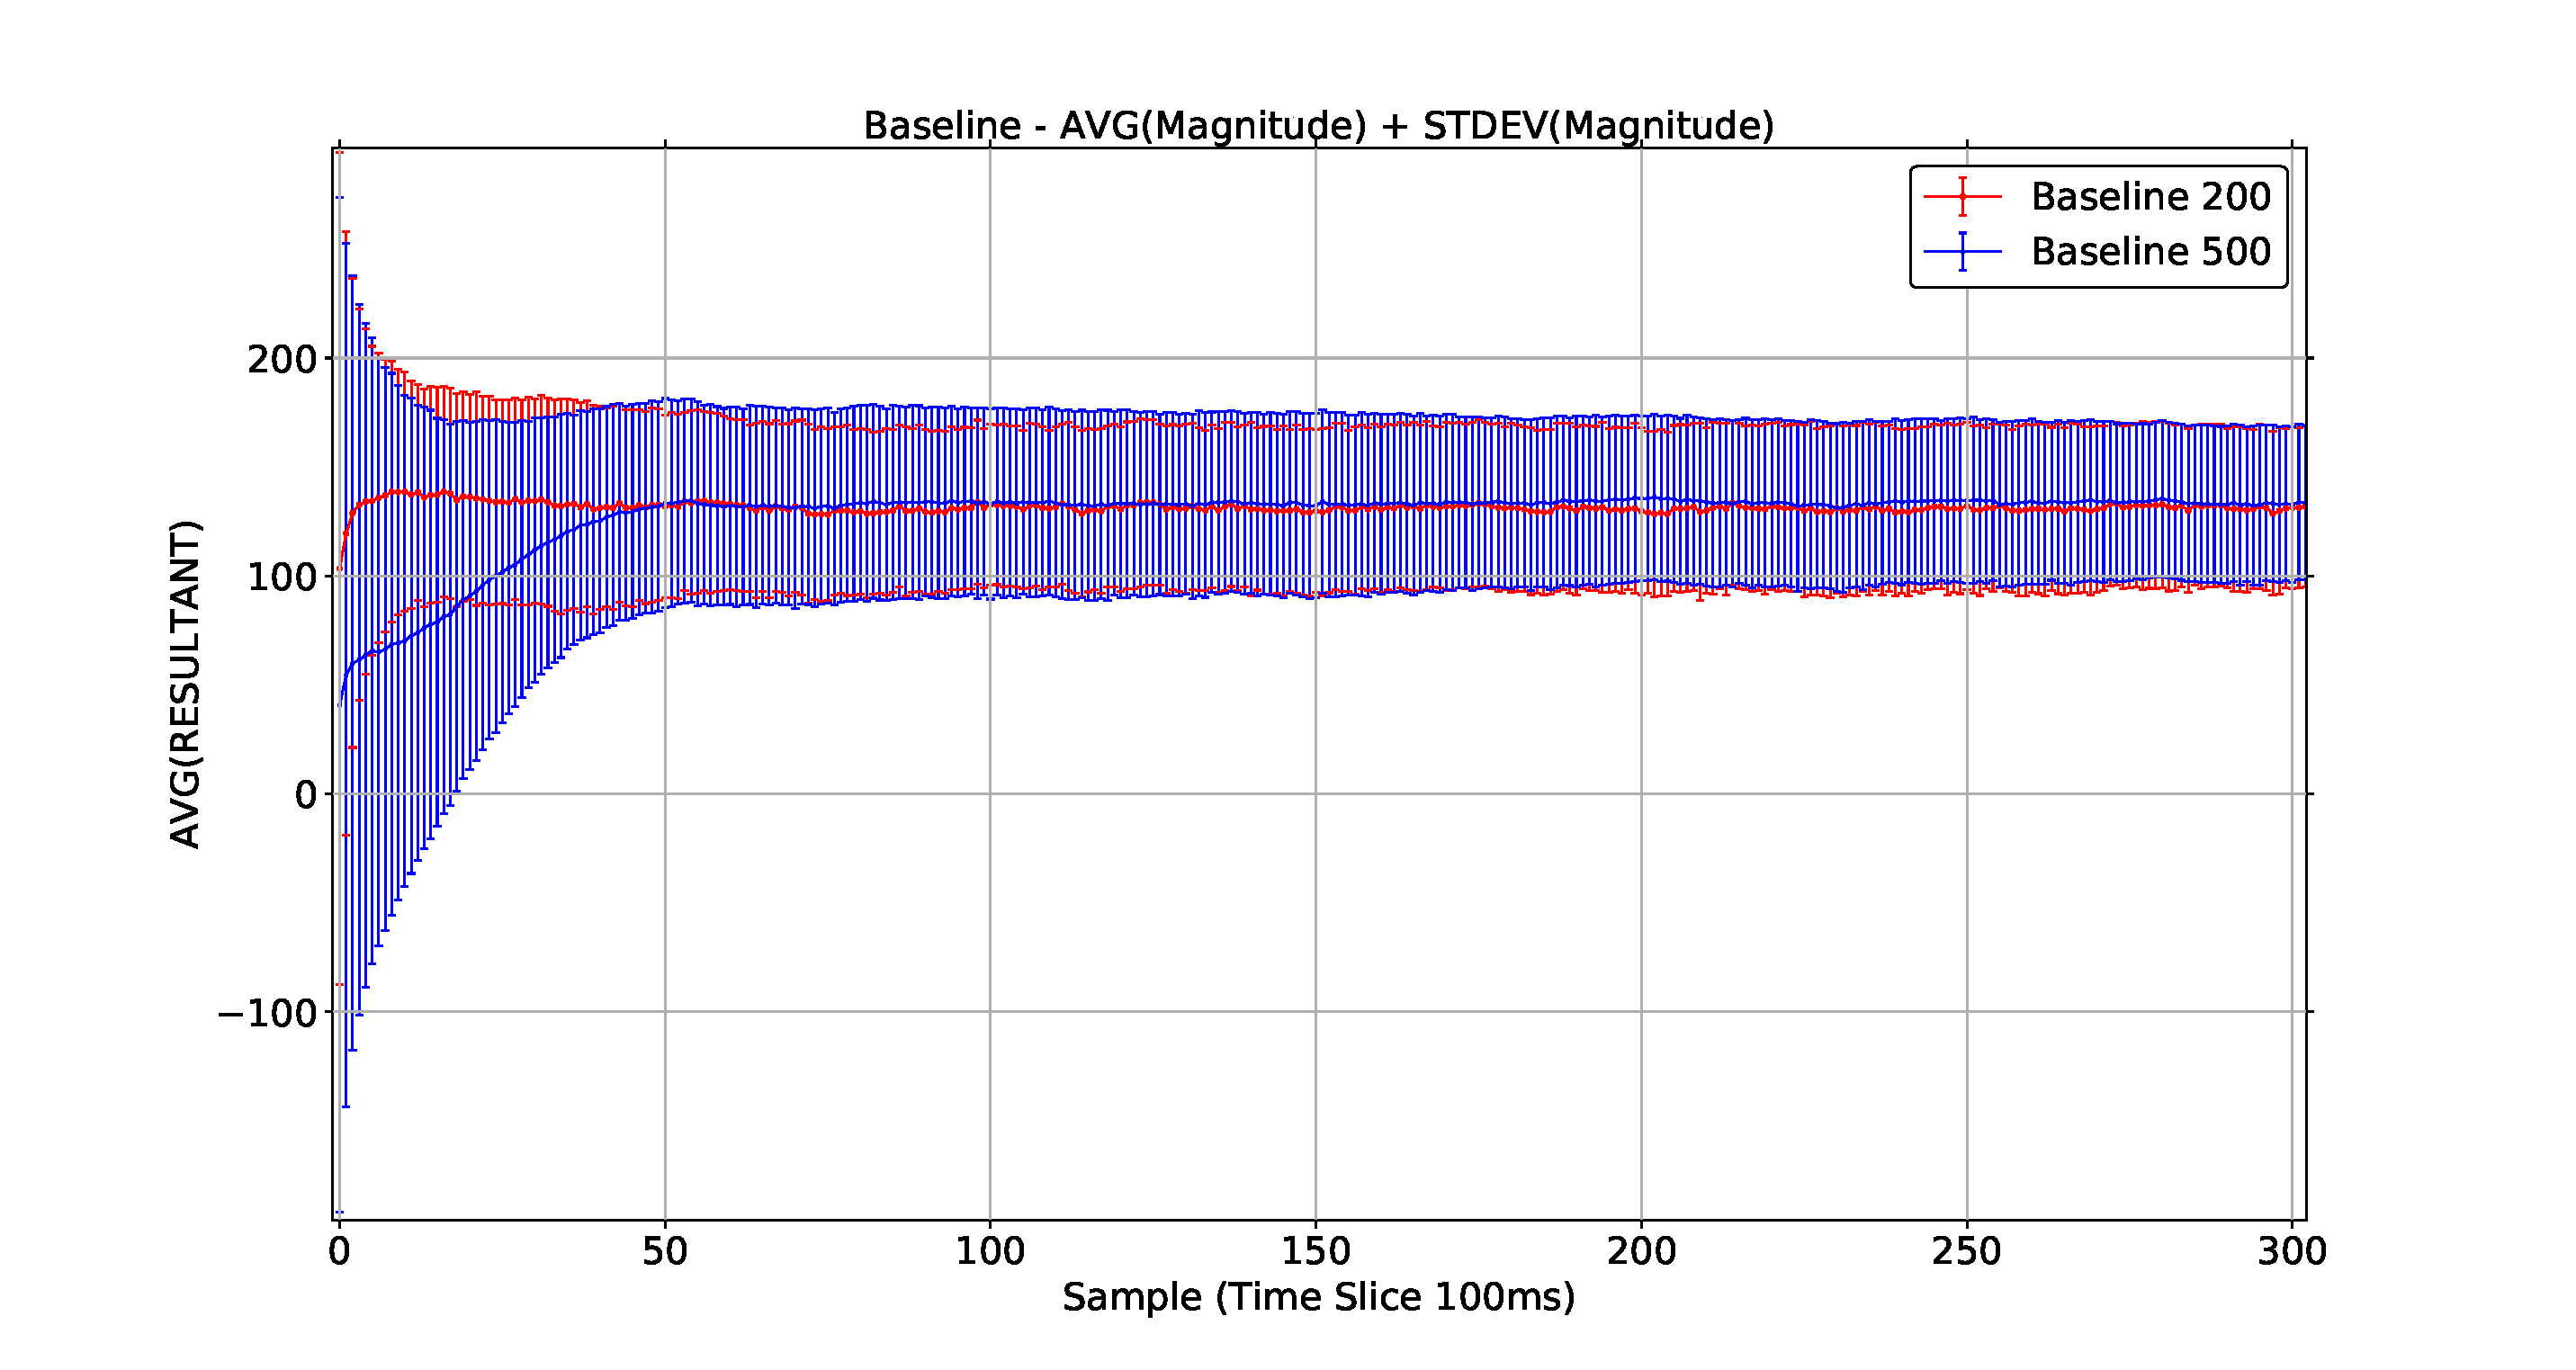
\includegraphics[width=13cm]{CHAPTER-5/figures/ArbitrarySize200500MAG}
\end{center}
\caption{Swarm size magnitude comparison\label{methods:ArbitrarySizeMag200500}}
\end{figure}

\autoref{methods:ArbitrarySizeMag200500} shows the average magnitude of the agents fluctuate while the swarm stabalises (disorganised stage) and eventually both swarms stabalise to comparable magnitudes and variations.

These two metrics show that the swarm is able to expand to its maximum distribution without being impeded. If the swarm's area was impeded the magnitude would not have been able to stabalise and would have remained high. The identification of swarm bound containment will be discussed in chapter~\ref{chapter:flooding}.

%% \subsection{Mobile swarm internal movement testing\label{section:swarmTesting}}
%% The results presented here show that the metric will identify changes in a swarm, this metric can therefore be applied to measure the resulting internal movement of the swarm when it is goal based. The metrics can also be used to identify the effects of negotiating obstacles or modifications to an algorithm to exploit a behaviour such as closing voids or surround an object.
%% 
%% With a stationary swarm the only influencing factors that need to be taken into consideration are the cohesion and repulsion of the agents. The most obvious change to the swarms algorithm is to include a directional bias. The most common way of applying the bias is to include a GPS sensor into each of the agents to provide a direction that is then used to apply a directional influence to the swarm. 
%% 


